\documentclass[12pt]{article}
\usepackage[spanish]{babel}
\usepackage{natbib}
\usepackage{url}
\usepackage[utf8]{inputenc}
\usepackage{amsmath}
\usepackage{graphicx}
\usepackage{parskip}
\usepackage{fancyhdr}
\usepackage{vmargin}
\usepackage[ddmmyy]{datetime}
\usepackage{anyfontsize}
\usepackage{helvet}
\renewcommand{\familydefault}{phv}
\usepackage{xcolor}

\usepackage{float}
\usepackage[section]{placeins}
\usepackage{tocloft}

% Alinear completamente el texto del índice de figuras al margen izquierdo
\setlength{\cftfigindent}{0pt}     % sin sangría a la izquierda
\setlength{\cftfignumwidth}{2em}   % ancho reservado para "Figura X"

\usepackage[T1]{fontenc}

\usepackage{arevmath}

% Definir tamaño por defecto para todas las figuras
\setkeys{Gin}{width=\textwidth, keepaspectratio}

\setmarginsrb{2.5 cm}{2.25 cm}{2.5 cm}{1.50 cm}
           {1 cm}{1.25 cm}{1 cm}{1.50 cm}

\usepackage{color}
\usepackage{hyperref}
\hypersetup{
    colorlinks=true, % set true if you want colored links
    linktoc=all,     % set to all if you want sections and subsections linked
    linkcolor=blue,  % choose some color if you want links to stand out
    urlcolor=blue,
}

\usepackage{subfig}

\usepackage{fancyvrb}
\fvset{xleftmargin=\mathindent}

% code blocks
\usepackage{verbatimbox}
\newenvironment{fullgrayverb}
{\verbbox}
{\endverbbox\par\colorbox{gray!25}{\parbox{\textwidth}{\theverbbox}}\par}

% inline code blocks
\usepackage{tcolorbox}
\newcommand\mystrut{\rule[-3pt]{0pt}{12pt}}
\newtcbox{\code}{on line, boxrule=0pt, boxsep=0pt, top=0pt,
left=0pt, bottom=0pt, right=0pt, colback=gray!25, colframe=white,
fontupper={\ttfamily\mystrut}}

\title{Análisis de Señales}          % Titulo del trabajo.
\author{Klöckner, Lema Roveta, Dei Castelli}
\newcommand{\padron}{123456, 123456}    % Padrón
\newcommand{\tpnumber}{1}       % Número de trabajo práctico
\date{\today}                   % Fecha (automática)

\makeatletter
\let\thetitle\@title
\let\theauthor\@author
\let\thedate\@date
\makeatother

\pagestyle{fancy}
\fancyhf{}
\rhead{\theauthor}
\lhead{\thetitle}
\cfoot{\thepage}

\begin{document}
\begin{titlepage}
    \vspace*{-2.5cm}
    {\centering
    
\includegraphics[width=1.00\textwidth]{logofiuba.png}\\[2.25 cm]}
    \centering
    \textsc{\Large TB065}\\[0.2 cm]
    \textsc{\large Señales y Sistemas}\\[4 cm]
    \textcolor{cyan}{{\fontsize{40}{60}\selectfont \bfseries \thetitle}}\\[0.5cm]
    {\Large \bfseries Trabajo Práctico Especial}\\[5cm]

    \vfill
    \noindent\makebox[\linewidth]{\rule{\textwidth}{0.4pt}}\\[0.5cm]
    \begin{minipage}{.50\textwidth}
    \textbf{Integrante}\\
    Martin Klöckner \\ Mateo Lema Roveta \\ Ernesto Dei Castelli
    \end{minipage}%
    \begin{minipage}{.25\textwidth}
    \textbf{Legajo}\\
    123456 \\ 
    123456 \\ 
    123456
    \end{minipage}%
    \begin{minipage}{.25\textwidth}
     \begin{flushright}
        \textbf{Correo electrónico}\\
         \href{mailto:mklockner@fi.uba.ar}{mklockner@fi.uba.ar} \\
         \href{mailto:mlema@fi.uba.ar}{mlema@fi.uba.ar} \\
         \href{mailto:edei@fi.uba.ar}{edei@fi.uba.ar}
    \end{flushright}
    \end{minipage}
\end{titlepage}

\setcounter{tocdepth}{2}
\hypersetup{linkcolor=black} % colorlinks=true option is used
\tableofcontents
\listoffigures
\pagebreak

\section{Introducción}

En el presente trabajo se realiza un análisis en el dominio temporal de en
principio dos señales musicales de muestra, en las cuales se buscan porciones
cuasi-periódicas y no periódicas, y luego se filtran utilizando dos filtros
diferentes.  Por último, se generan mediante simulación de tres instrumentos
musicales diferentes, tres señales, las cuales se analizan y comparan las formas
de onda generadas.

\hypertarget{dominio-temporal}{%
\section{Dominio temporal}\label{dominio-temporal}}

\hypertarget{primer-muestra}{%
\subsection{Primer muestra}\label{primer-muestra}}

Para la primer muestra (archivo cancion1.wav) se realiza el
gráfico de la misma en el dominio temporal, el resultado se muestra en
la figura 1.

La frecuencia de muestreo de la misma es 44100 Hz, esto se obtiene del
mismo script utilizado para graficar el archivo, en el cual se divide la
cantidad de muestras por la duración del archivo.

\begin{figure}
\centering
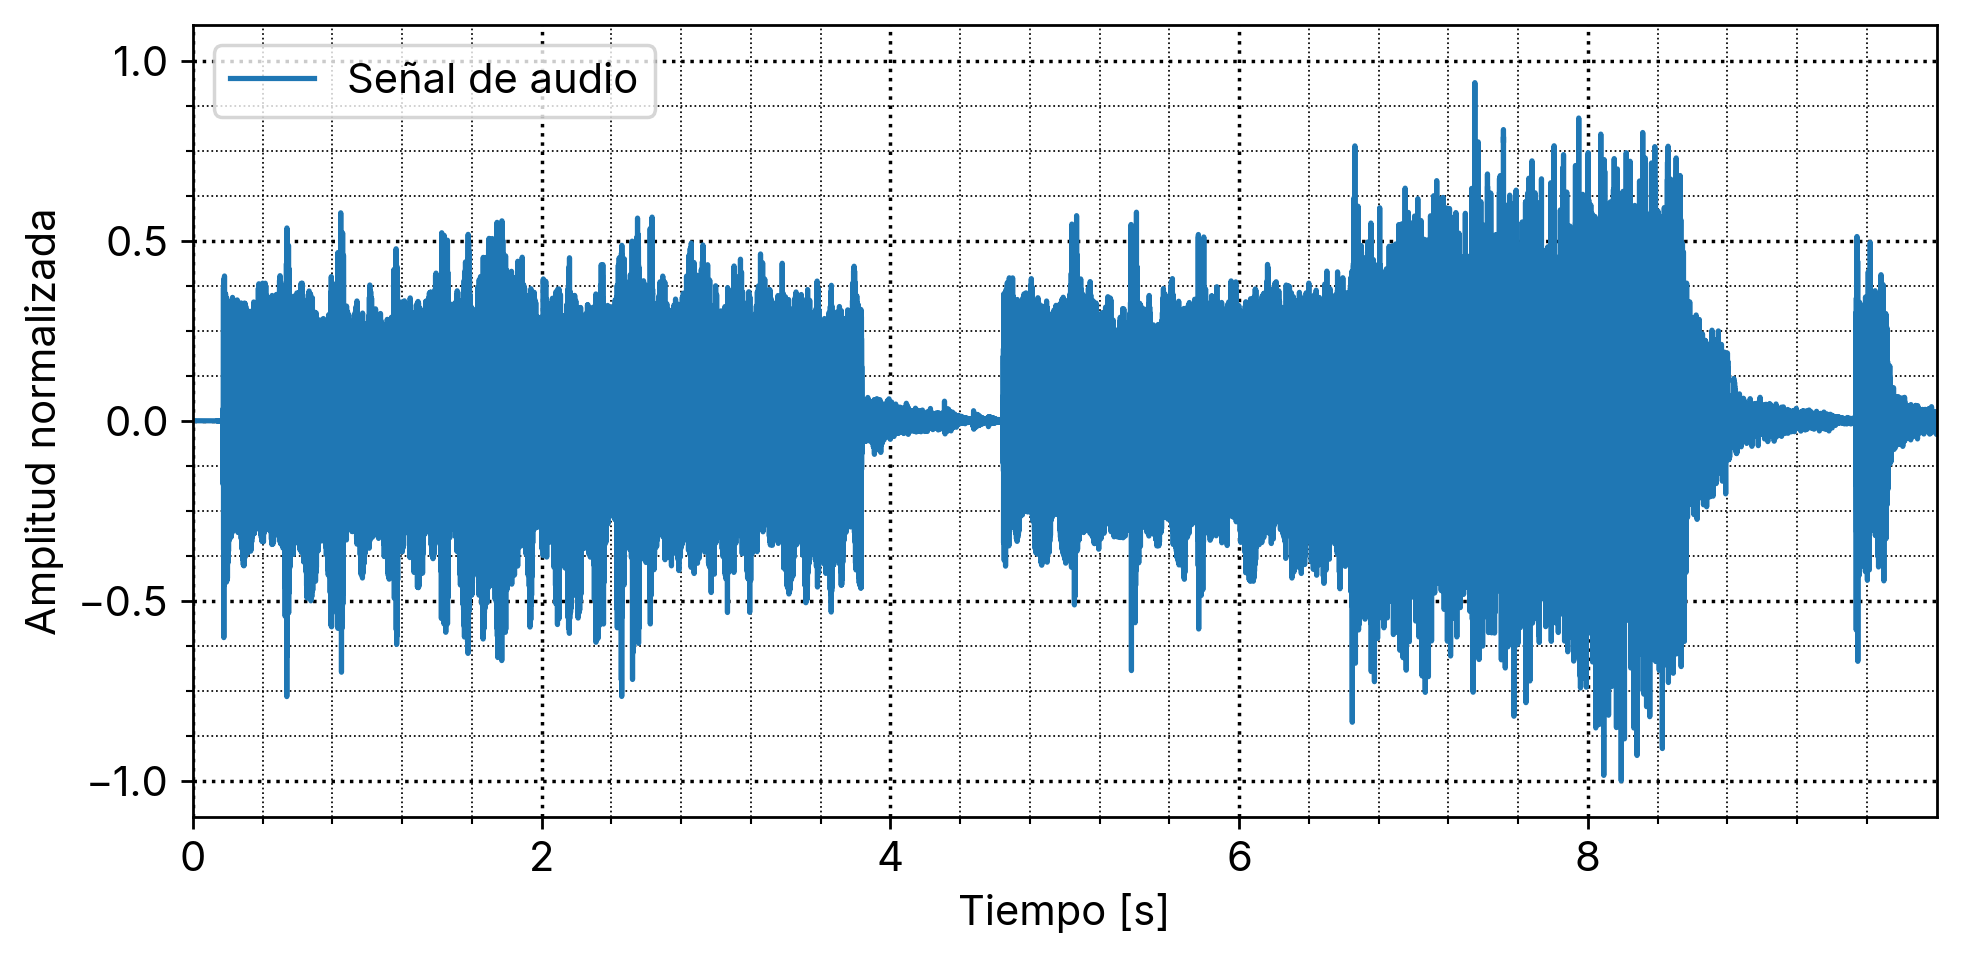
\includegraphics{plot/cancion1.png}
\caption{Gráfico de archivo `cancion1.wav'}
\label{cancion1}
\end{figure}

\hypertarget{secciones-cuasi-periuxf3dicas}{%
\subsubsection{Secciones
cuasi-periódicas}\label{secciones-cuasi-periodicas}}

Cuando la señal tiene una estructura repetitiva, pero con variaciones en
amplitud, fase o frecuencia se dice que la señal es cuasi-periódica.

Realizando un análisis visual en detalle de la muestra se buscan partes
donde se comporte como tal, dos ejemplos se dan en las figuras 2 y 3. En
la primera se gráfica el intervalo \(0.248\) s a \(0.256\) s, mientras
que en la segunda se gráfica el intervalo \(0.520\) s a \(0.528\) s.

\begin{figure}
\centering
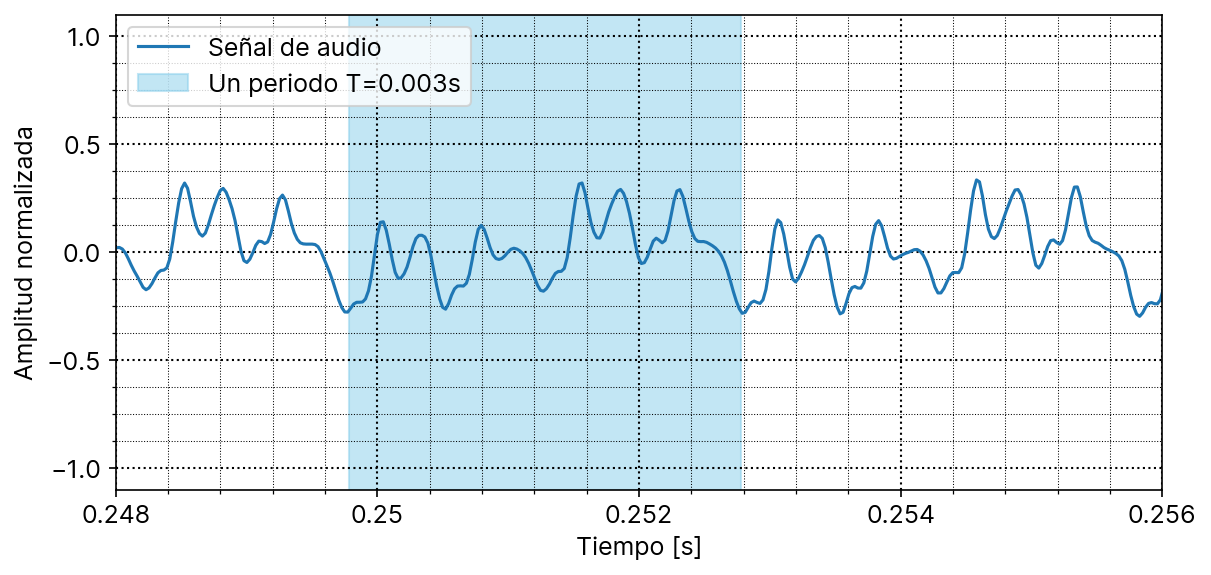
\includegraphics{plot/cancion1_0_248s_a_0_256s.png}
\caption{Sección cuasi-periódica archivo `cancion1.wav'}
\label{cancion1_seccion_cuasi_periodica}
\end{figure}

Dentro de los intervalos cuasi-periódicos graficados, se pueden detectar
visualmente los períodos fundamentales, los cuales se ven resaltados en
color celeste claro.

Curiosamente en ambos casos el período es igual y resulta \(T=0.003\) s,
lo cual corresponde con una frecuencia de aproximadamente \(333\) Hz.
Comparando con notas musicales de tabla esto se asemeja a una nota
\emph{E4}, la cual tiene una frecuencia de \(329.228\) Hz. Siendo que el
período se relaciona de manera inversa con la frecuencia y esta de
manera directa con la nota musical, se puede asegurar que al disminuir
este período la frecuencia aumentará y la nota musical será mas aguda,
mientras que en el caso contrario si aumenta el período la frecuencia
disminuye y también la nota musical.

\begin{figure}
\centering
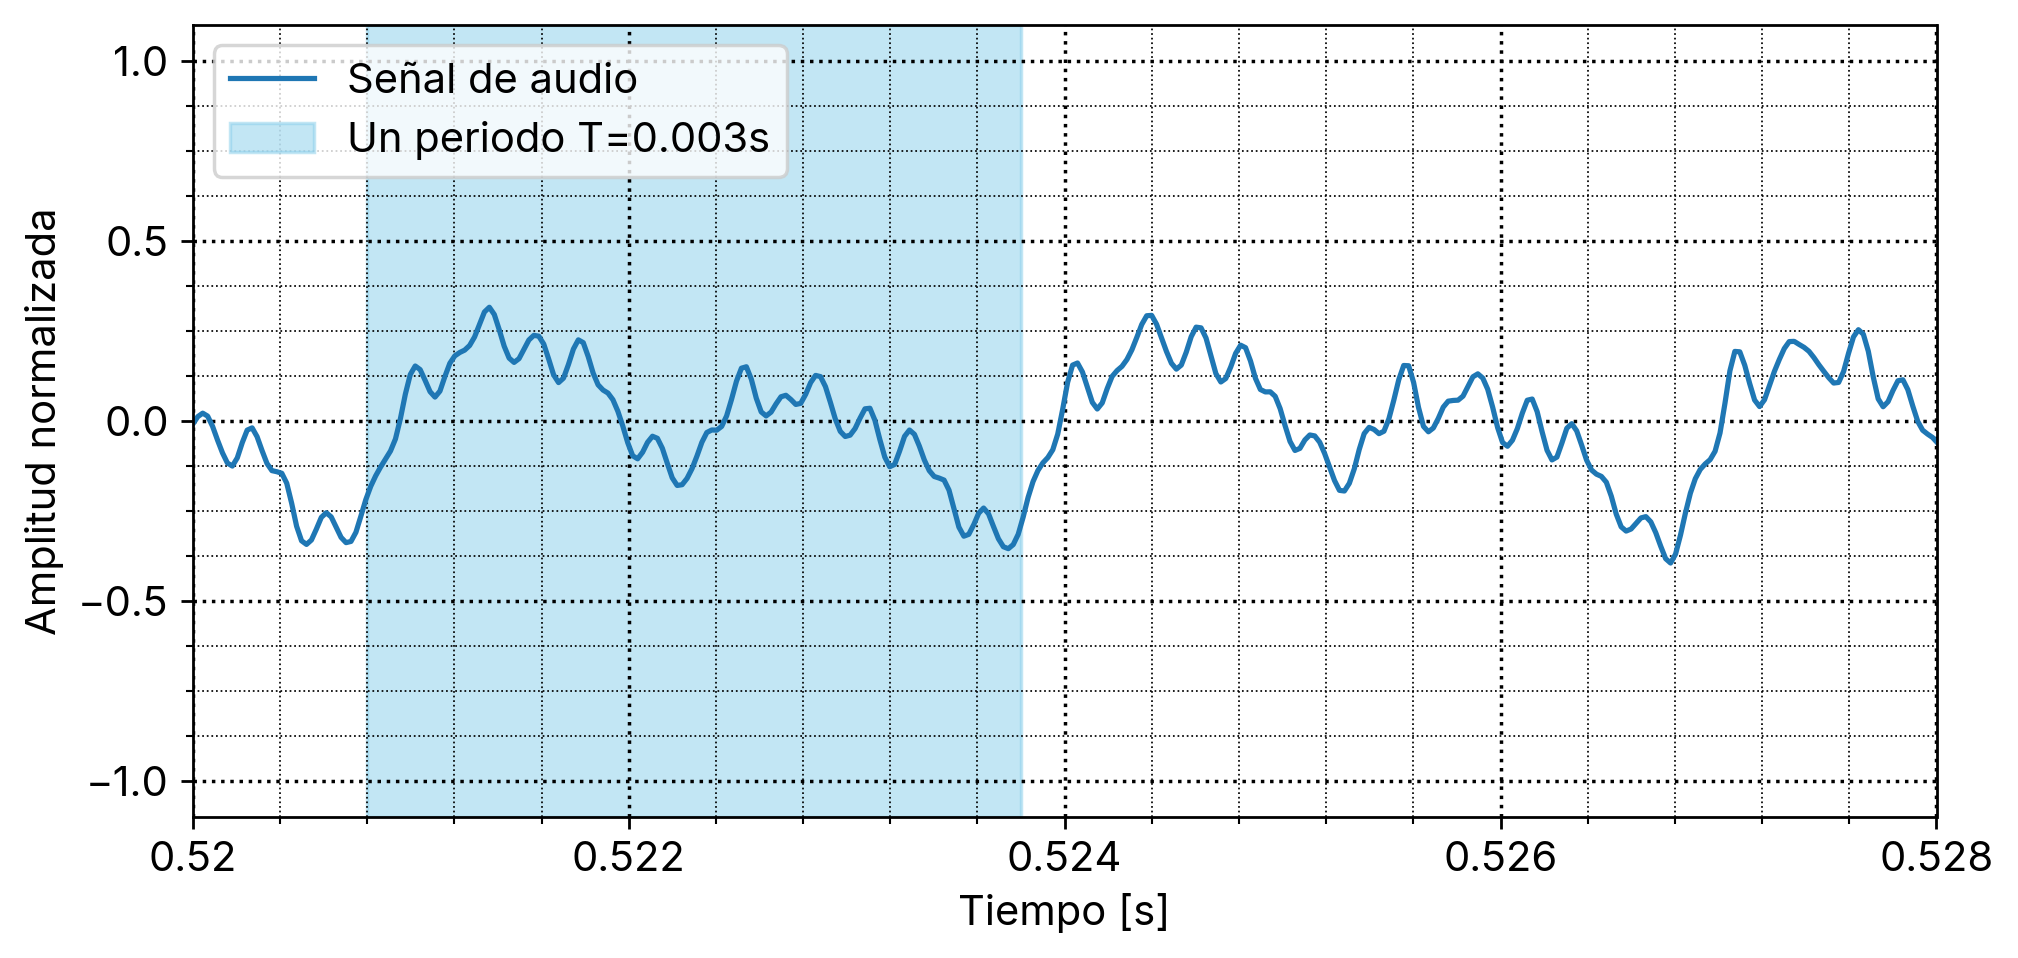
\includegraphics{plot/cancion1_0_520s_a_0_528s.png}
\caption{Otra sección cuasi-periódica archivo `cancion1.wav'}
\label{cancion1_seccion_cuasi_periodica2}
\end{figure}

\hypertarget{segunda-muestra}{%
\subsection{Segunda muestra}\label{segunda-muestra}}

Utilizando el mismo script de python utilizado para la primer muestra
(archivo cancion1.wav) se gráfica la señal de la segunda
muestra (correspondiente al archivo cancion2.wav) en el dominio
temporal, en este caso se gráfica a partir del segundo 6 ya que antes de
esto la señal tiene amplitud nula, con lo cual no aporta información
significativa, el gráfico resultante se muestra en la figura 4.

La frecuencia fundamental de esta segunda muestra resulta \(48000\) Hz,
esto también se obtiene del script de python.

\begin{figure}
\centering
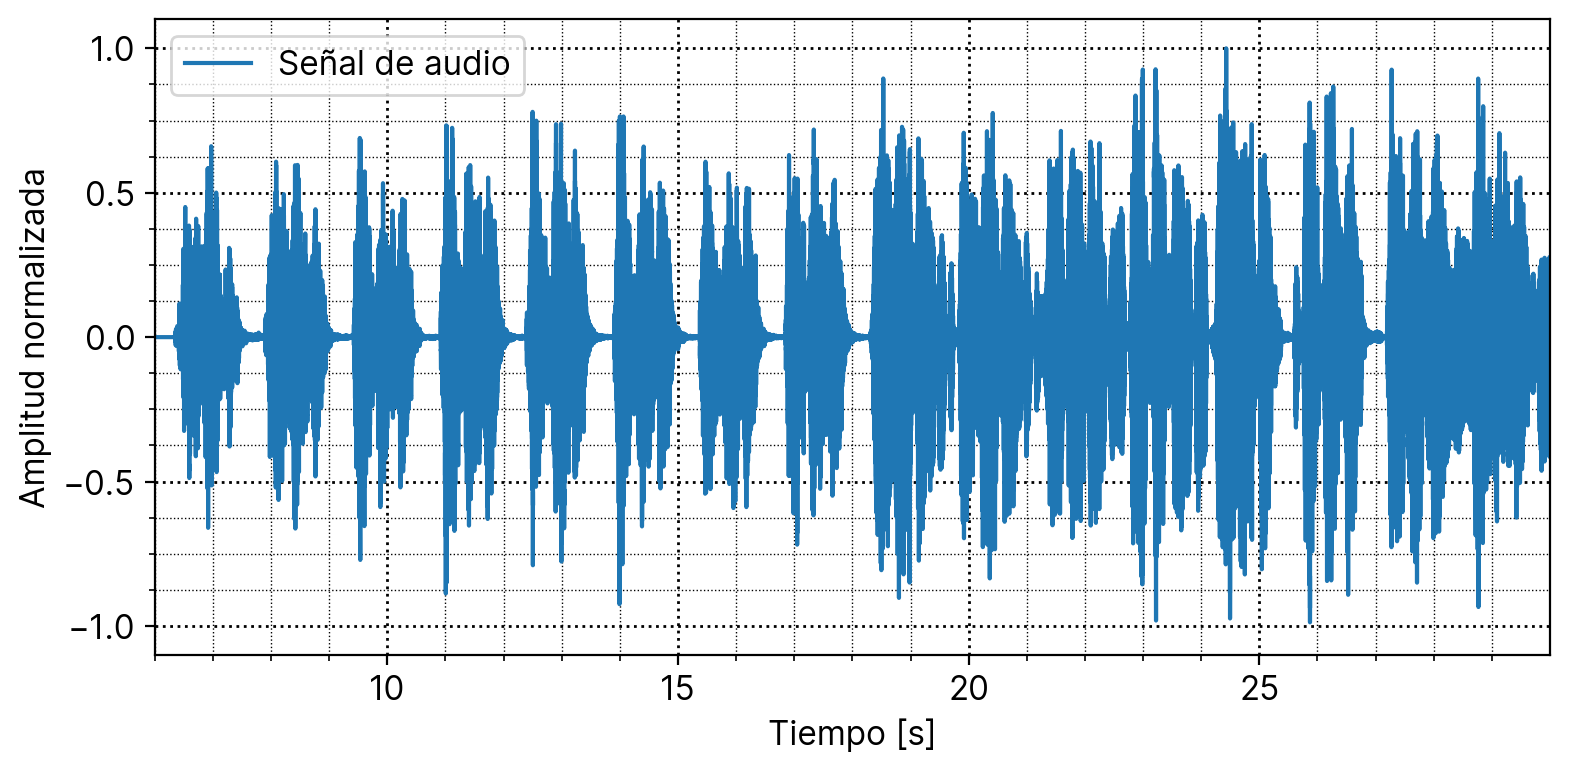
\includegraphics{plot/cancion2.png}
\caption{Gráfico de archivo `cancion2.wav'}
\label{cancion2}
\end{figure}

\hypertarget{secciones-no-periodicas}{%
\subsubsection{Secciones no-periódicas}\label{secciones-no-periodicas}}

A diferencia del análisis realizado sobre la primer muestra en busca de
secciones cuasi-periódicas, para esta segunda muestra se buscan
secciones no periódicas, esto es, secciones donde la señal no tiene un
patron repetitivo marcado. Se toman dos intervalos en los cuales la
señal de muestra se comporta como tal, el intervalo de \(14.72\) s a
\(14.73\) s y el intervalo \(26.57\) s a \(26.58\) s, ambos intervalos
se muestran graficados en las figura 5 y 6 respectivamente.

\begin{figure}
\centering
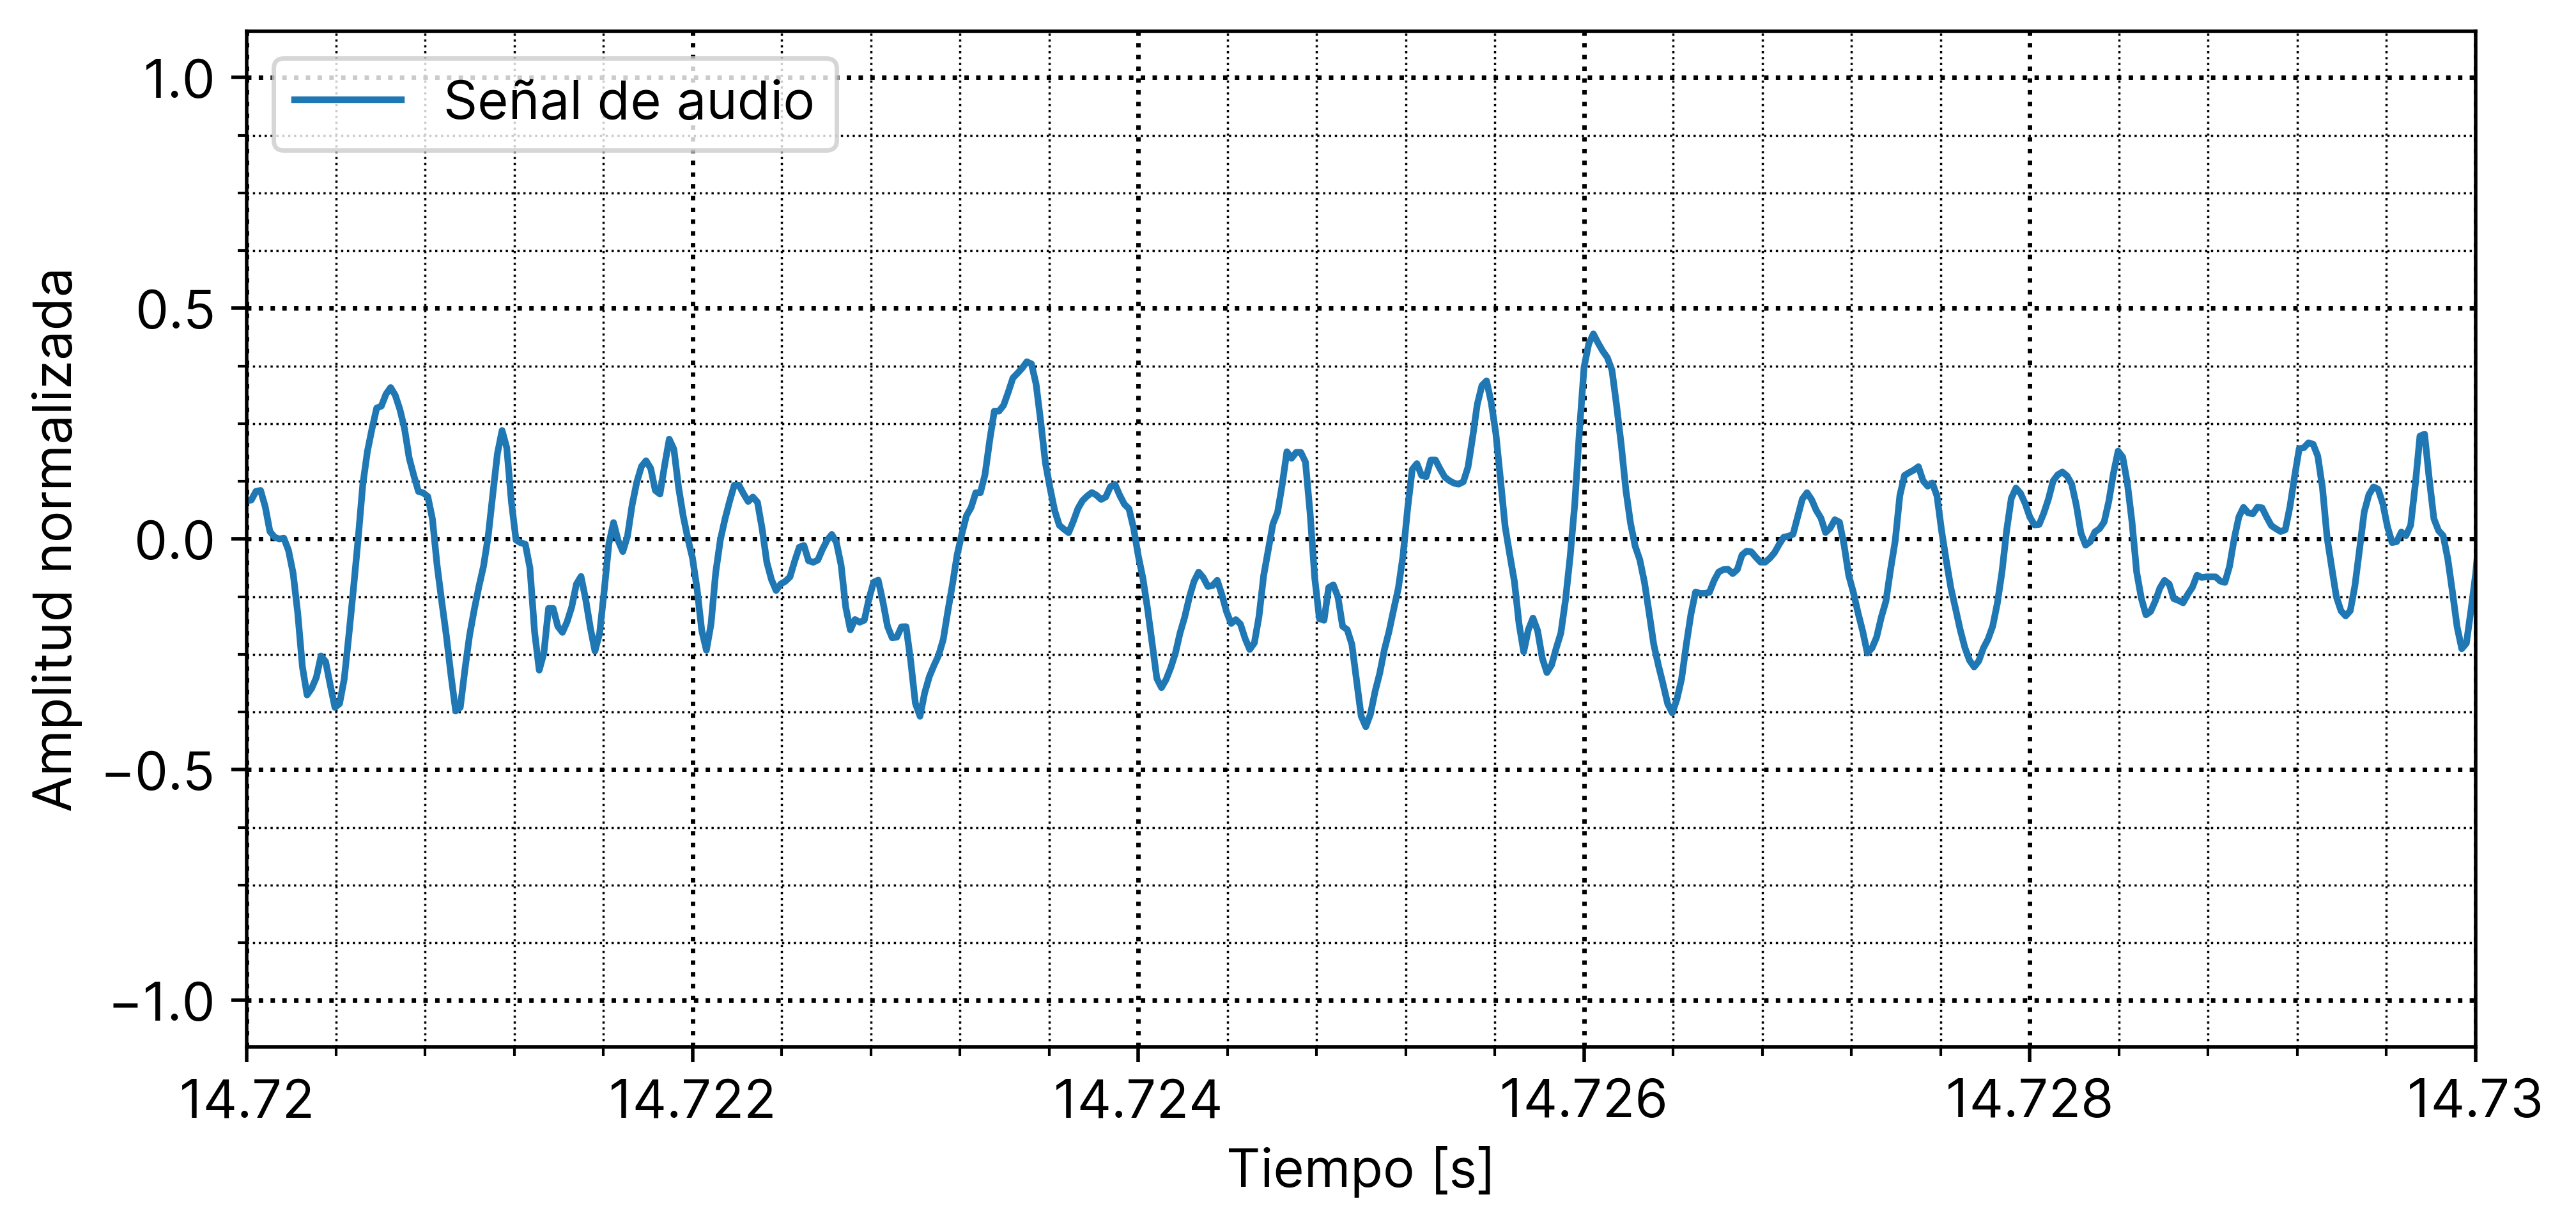
\includegraphics{plot/cancion2_14_72s_a_14_73s.png}
\caption{Sección no periódica archivo `cancion2.wav'}
\label{cancion2_seccion_no_periodica}
\end{figure}

\begin{figure}
\centering
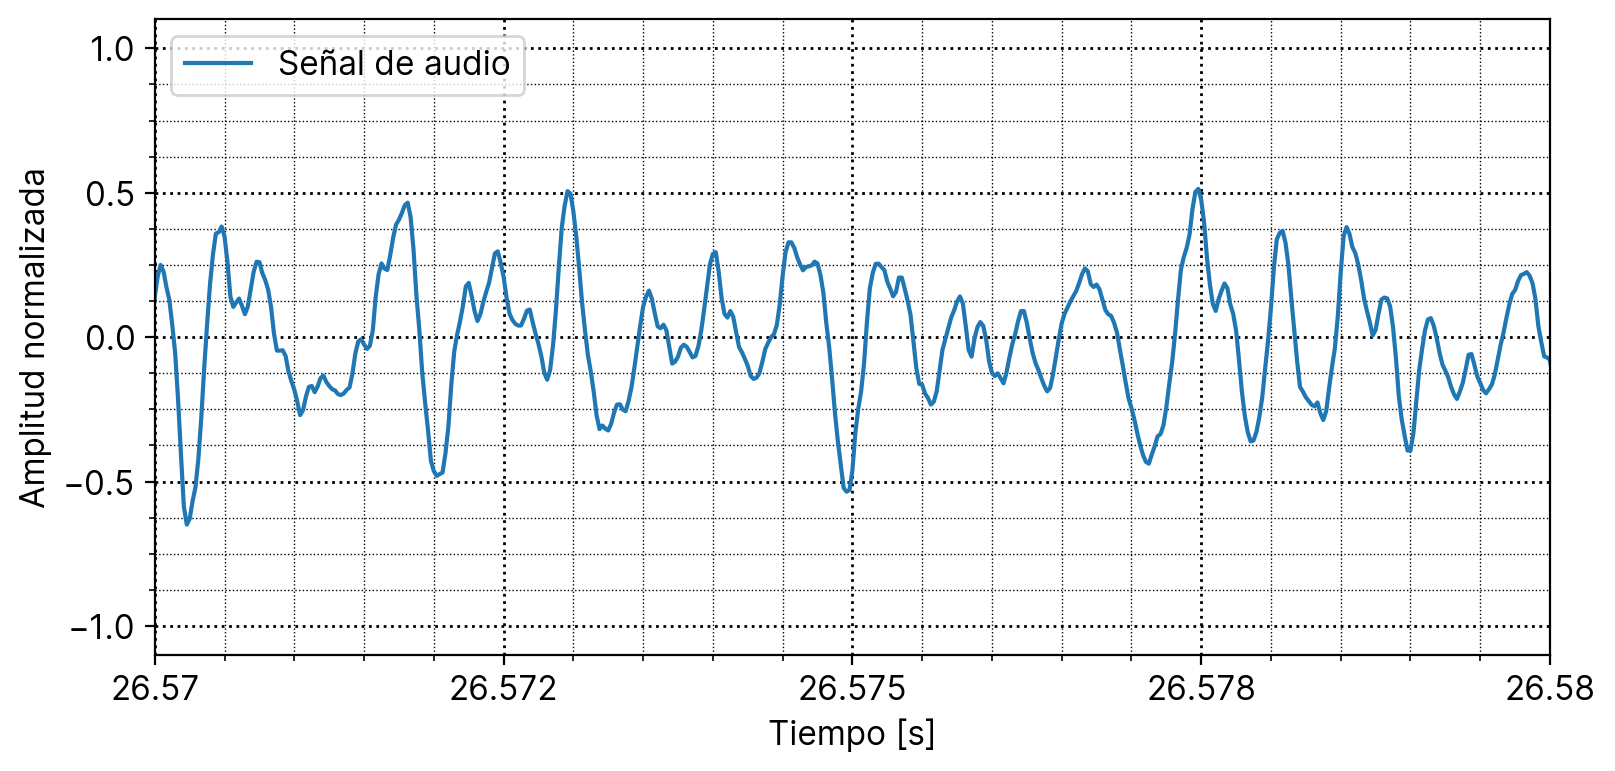
\includegraphics{plot/cancion2_26_57s_a_26_58s.png}
\caption{Otra sección no periódica archivo `cancion2.wav'}
\label{cancion2_seccion_no_periodica2}
\end{figure}

Dado que las secciones son no periódicas, no se puede hablar de una
frecuencia fundamental como si se podía en las secciones
cuasi-periódicas en la primer muestra.





\hypertarget{filtrado}{%
\subsection{Filtrado}\label{filtrado}}

Para obtener la salida de la señal luego de pasarla por un filtro
(respuesta al impulso del primer filtro correspondiente al archivo
respuesta\_impulso\_1.txt y del segundo filtro correspondiente
al archivo respuesta\_impulso\_2.txt) es necesario realizar una
convolución entre la señal de entrada y la respuesta al impulso del
filtro, esto suponiendo que el filtro es un sistema LTI (si no lo fuera
no se podría calcular la salida solo teniendo la respuesta al impulso).

La salida del filtro 1 al aplicar la primer muestra se puede ver en la
figura \ref{cancion1_filter1_output_compare}, en este gráfico de la señal completa se observa que atenúa partes de la señal y
amplifica otras, en particular amplifica principalmente antes del
segundo \(6\) y atenúa drásticamente luego. En mayor detalle como se observa en la figura \ref{cancion1_filter1_output_compare_0_248_a_0_256} para el intervalo entre 0.248 y 0.256 segundos, se ve como actúa sobre la señal amplificando partes de la misma.

\begin{figure}[H]
\centering
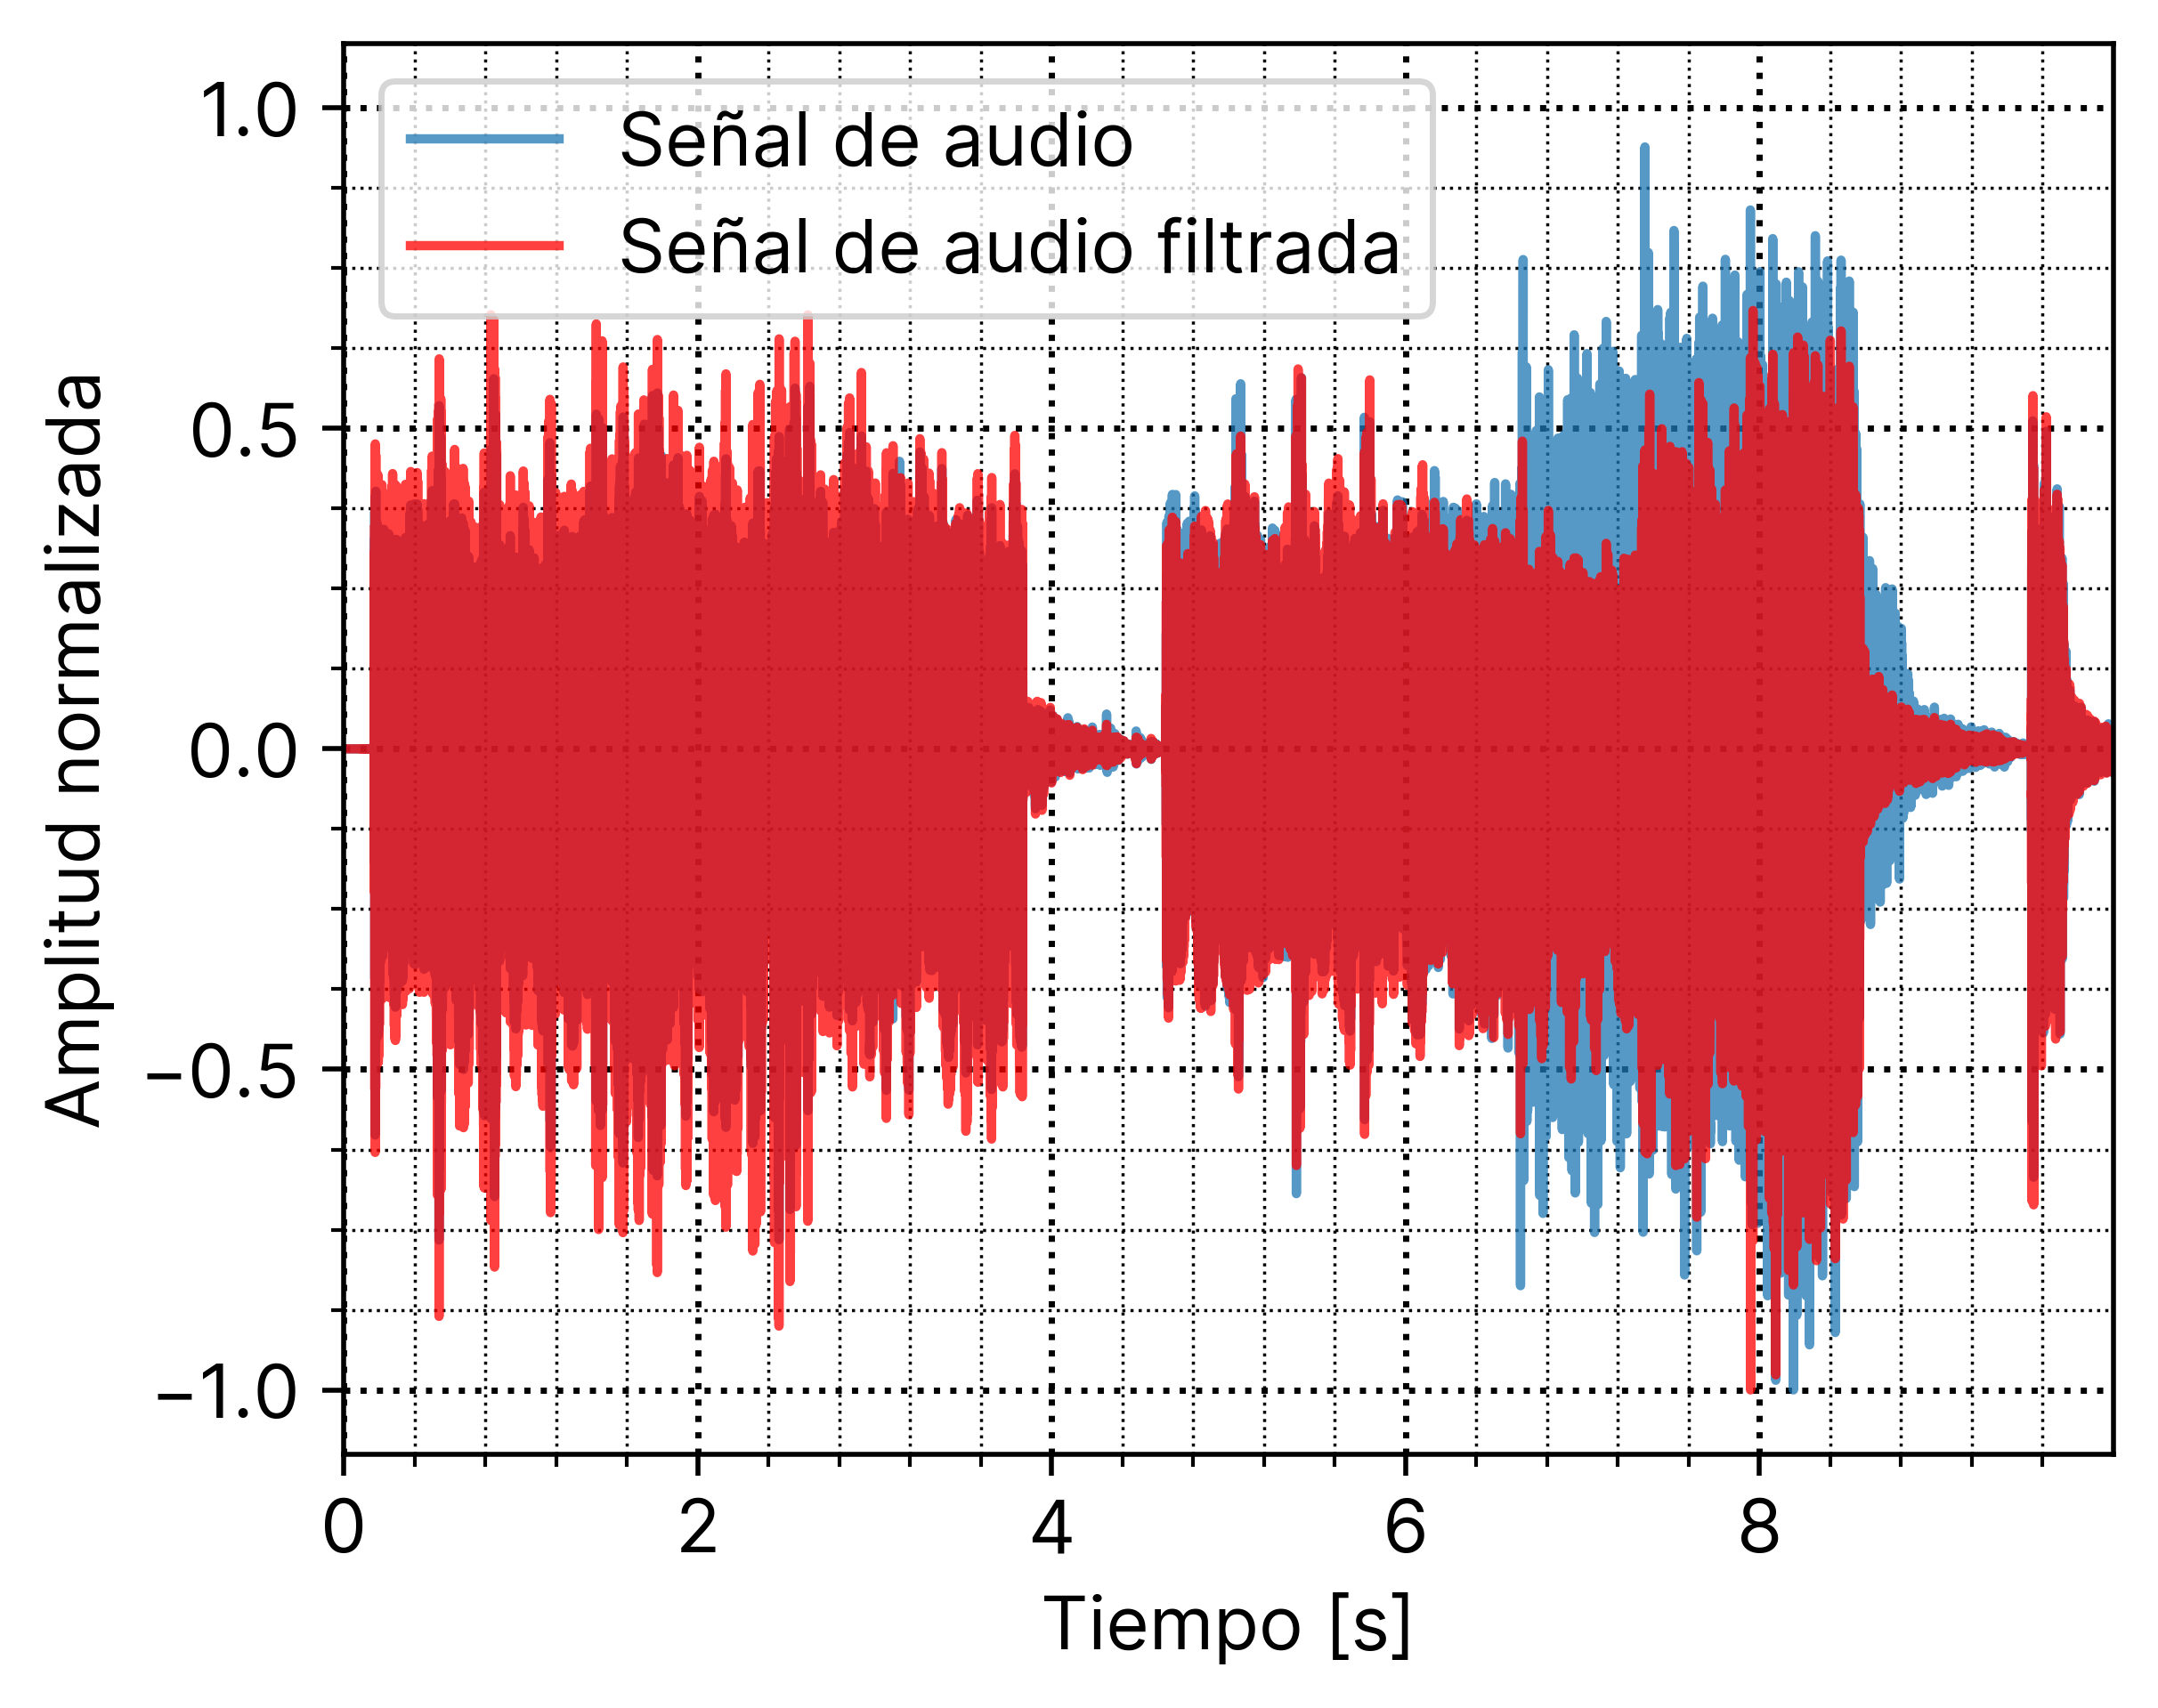
\includegraphics{plot/cancion1_filter1_output_compare.png}
\caption{Primer muestra salida de filtro 1}
\label{cancion1_filter1_output_compare}
\end{figure}

\begin{figure}[H]
\centering
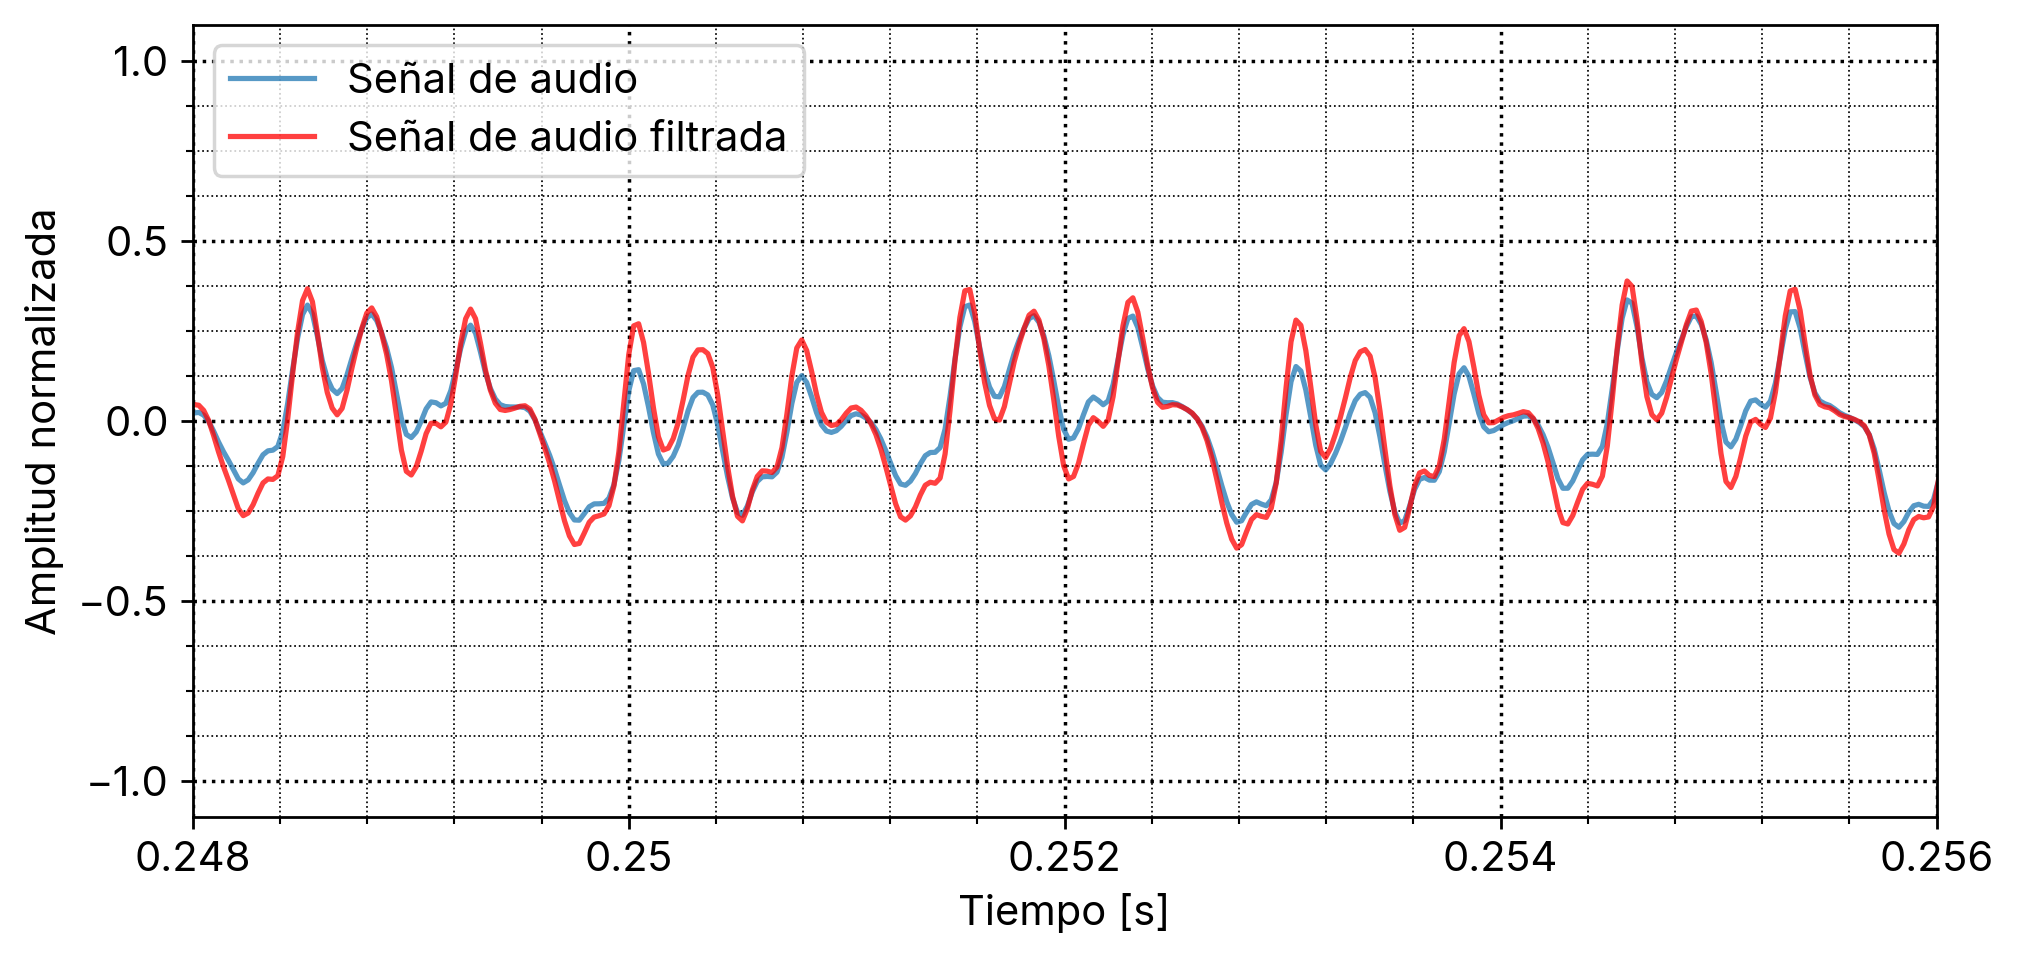
\includegraphics{plot/cancion1_filter1_output_compare_0_248_a_0_256.png}
\caption{Primer muestra salida de filtro 1 intervalo 0.248 a 0.256s}
\label{cancion1_filter1_output_compare_0_248_a_0_256}
\end{figure}

Aplicando el segundo filtro a la primer muestra resulta como se muestra
en el gráfico de figura \ref{cancion1_filter2_output_compare}. 
En esta figura de la señal completa Se puede ver que esta a diferencia del filtro 1, no atenúa o amplifica significativamente partes de la señal, si no
que realiza una leve atenuación de toda la señal. Analizando en detalle como se ve en la figura \ref{cancion1_filter2_output_compare_0_248_a_0_256} se puede ver el suavizado que realiza este filtro sobre la señal, esto sugiere que el filtro 2 es del tipo pasa bajos, ya que atenúa la frecuencias altas componentes en la señal original, haciendo que la señal resultante no tenga cambios abruptos.

\begin{figure}[H]
\centering
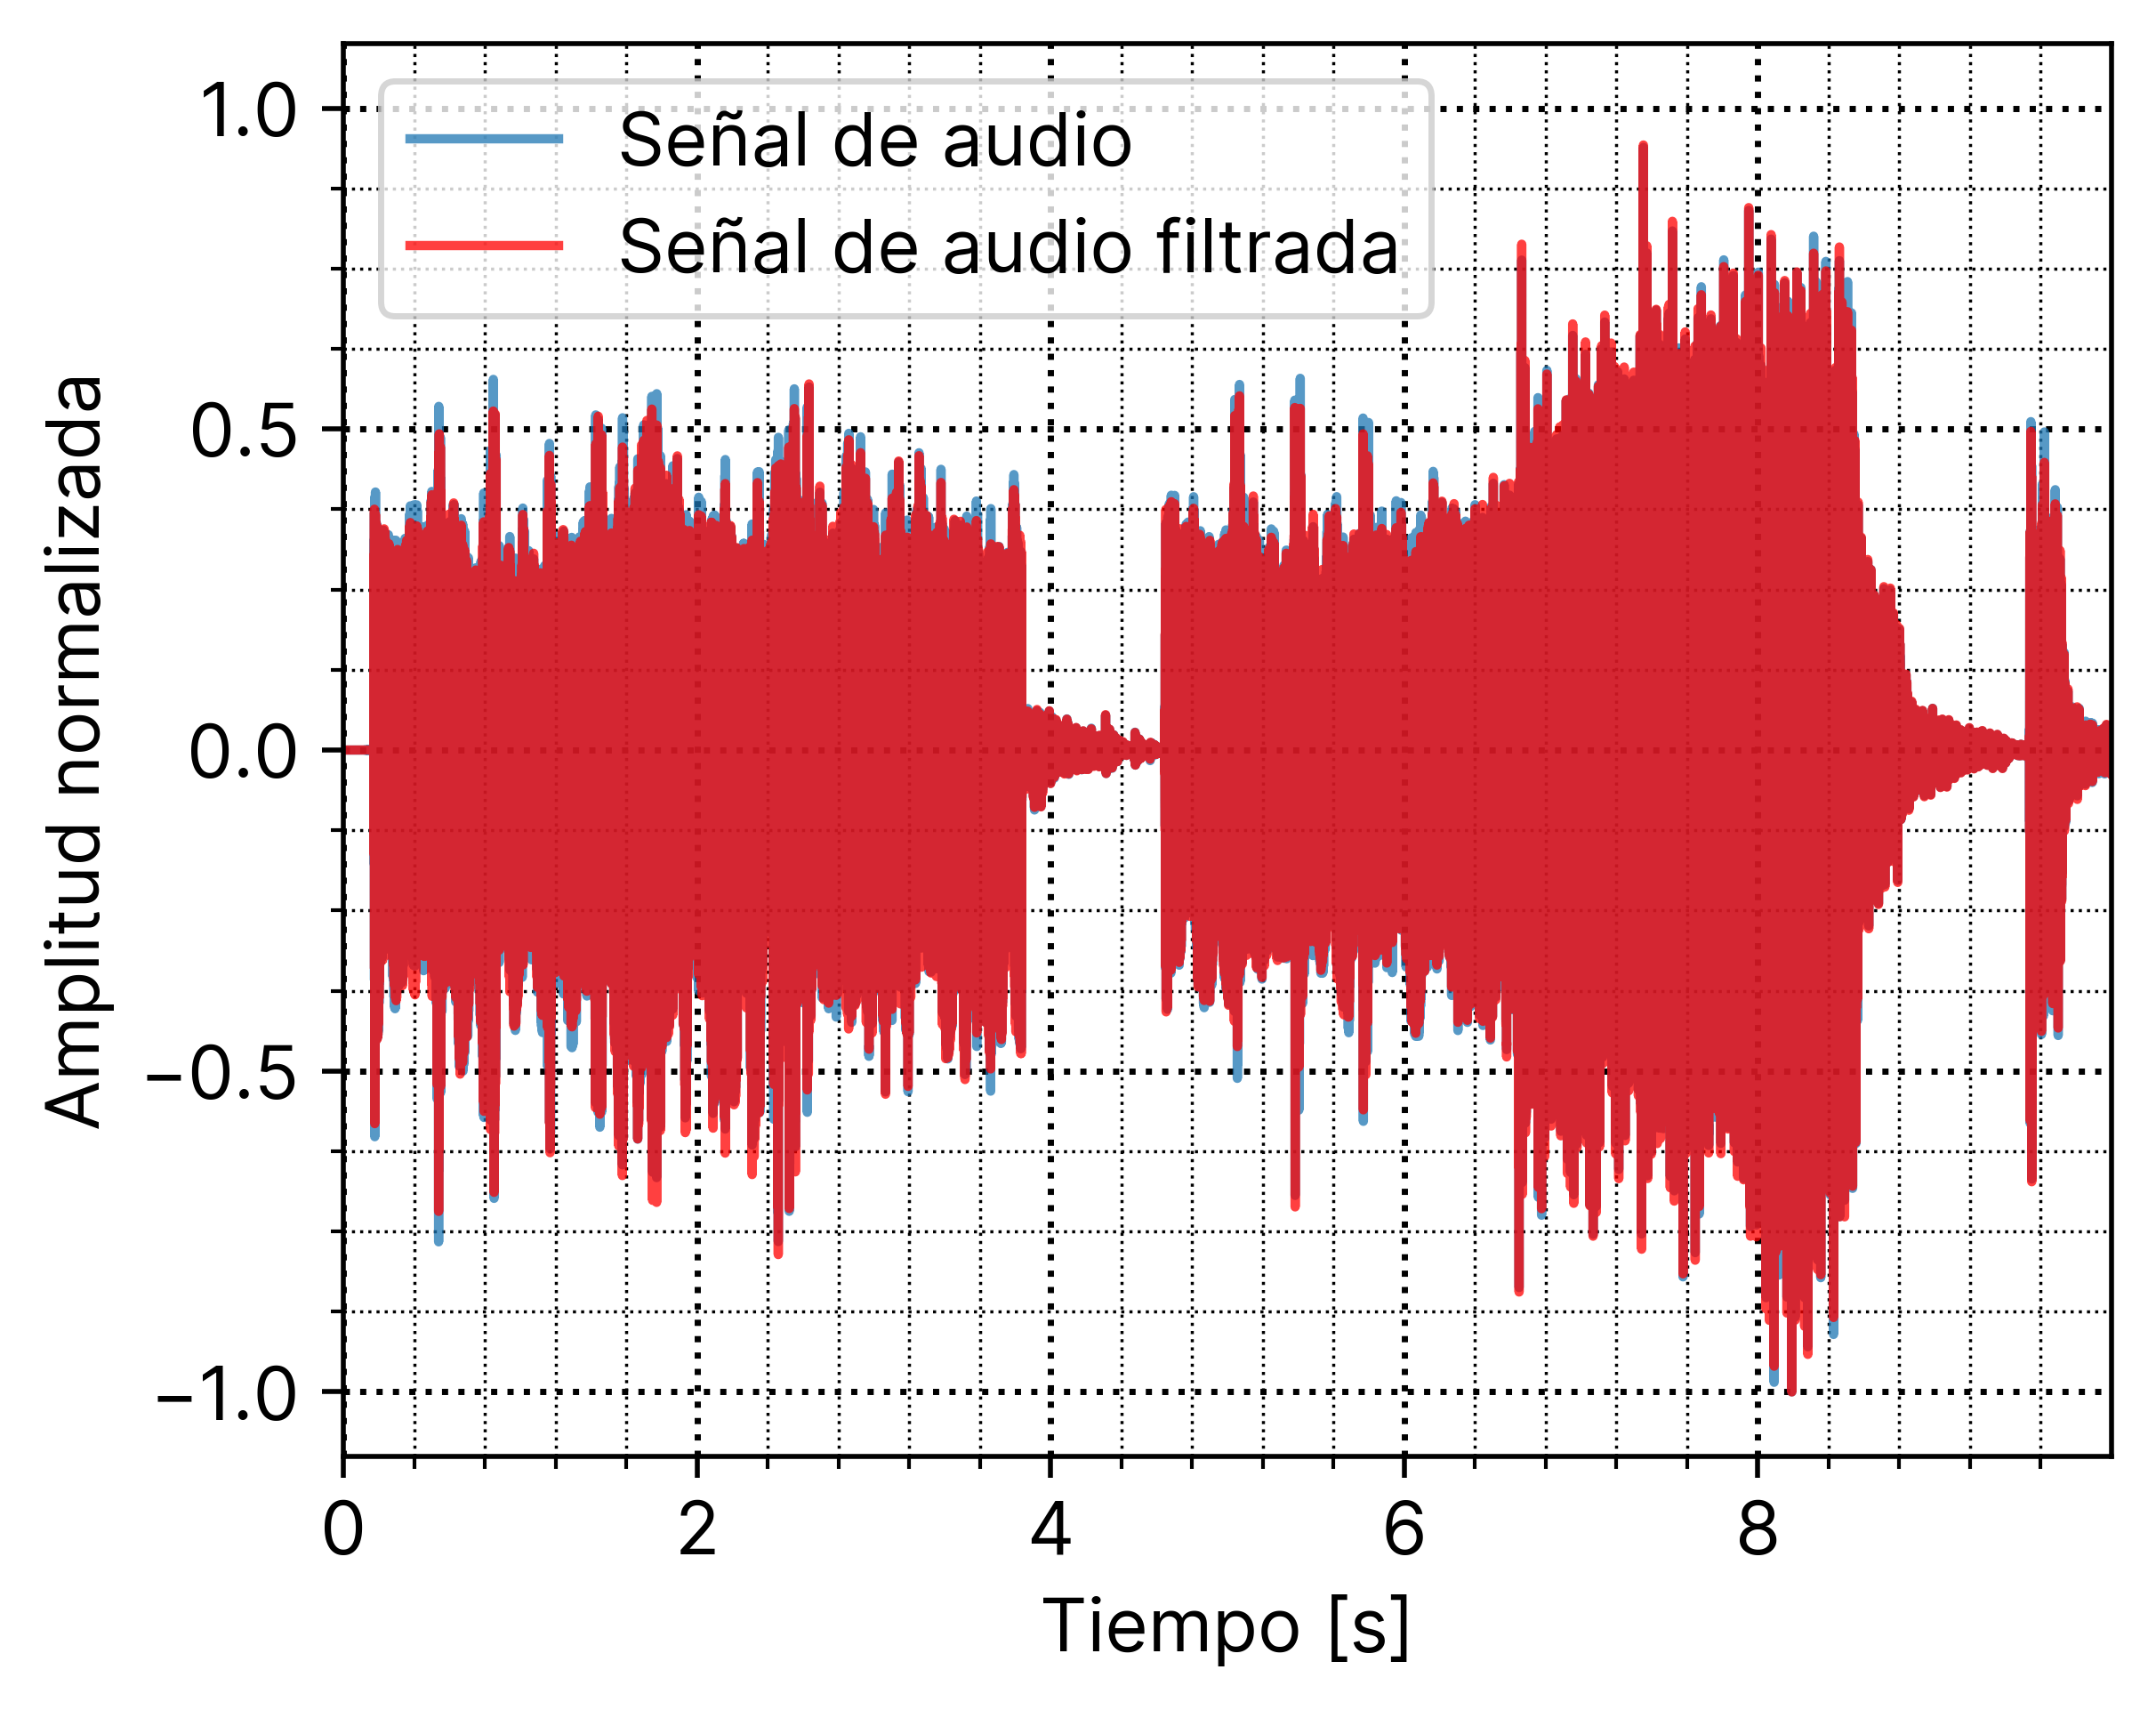
\includegraphics{plot/cancion1_filter2_output_compare.png}
\caption{Primer muestra salida de filtro 2}
\label{cancion1_filter2_output_compare}
\end{figure}

\begin{figure}[H]
\centering
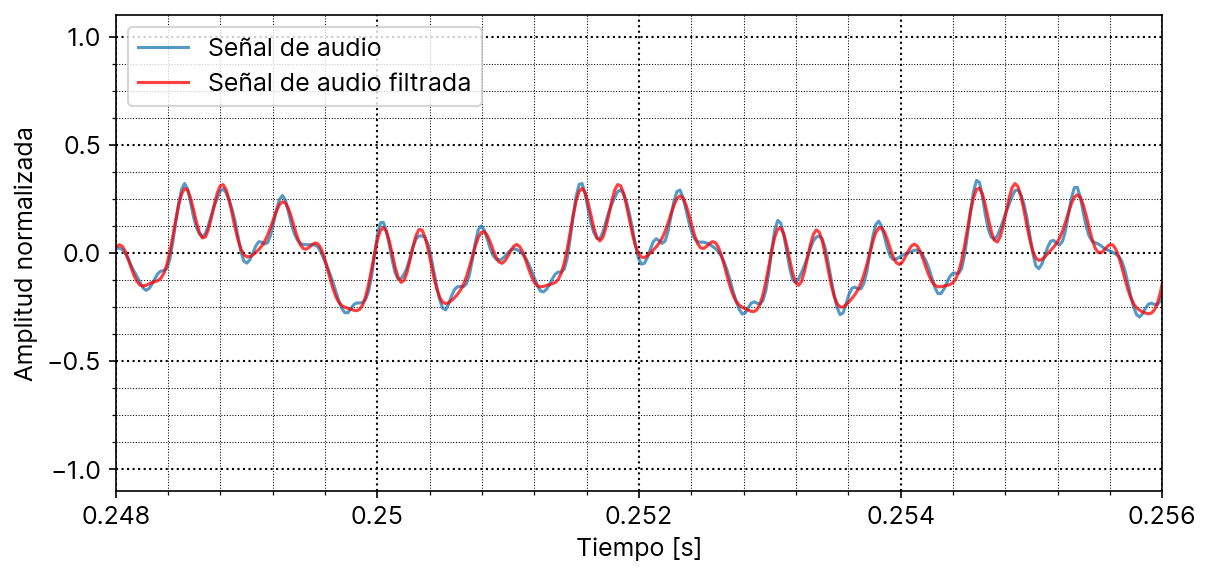
\includegraphics{plot/cancion1_filter2_output_compare_0_248_a_0_256.png}
\caption{Primer muestra salida de filtro 2 intervalo 0.248 a 0.256s}
\label{cancion1_filter2_output_compare_0_248_a_0_256}
\end{figure}

\pagebreak

De manera análoga para la segunda muestra se aplican los filtros mediante la
convolución entre la señal y la respuesta al impulso del respectivo filtro.

La salida de la segunda muestra al aplicar el primer filtro se puede ver en la
figura \ref{cancion2_filter1_output_compare} en la cual se gráfica la señal
completa y se aprecia como se atenúa la mayor parte, principalmente en la
primera mitad (antes del segundo 18.5 aproximadamente) y en menor medida en
la mitad restante, aunque en partes de la segunda mitad se atenúa drásticamente
de todas formas, como por ejemplo en el segundo 29 en el que se atenúa
aproximadamente un 70\% de la señal.

En la figura \ref{cancion2_6s_filter1_output_compare_26_57_a_26_58} se analiza
en mayor detalle la señal, en este caso el intervalo entre 26.57 y 26.58
segundos, en esta figura se observa como amplifica partes de la señal, en
particular, se observa que amplifica los picos en donde la señal tiene cambios
abruptos, es decir, donde la señal se compone de frecuencias altas, esto sugiere
que el primer filtro es del tipo pasa altos, es decir atenúa las frecuencias
bajas.

\begin{figure}
\centering
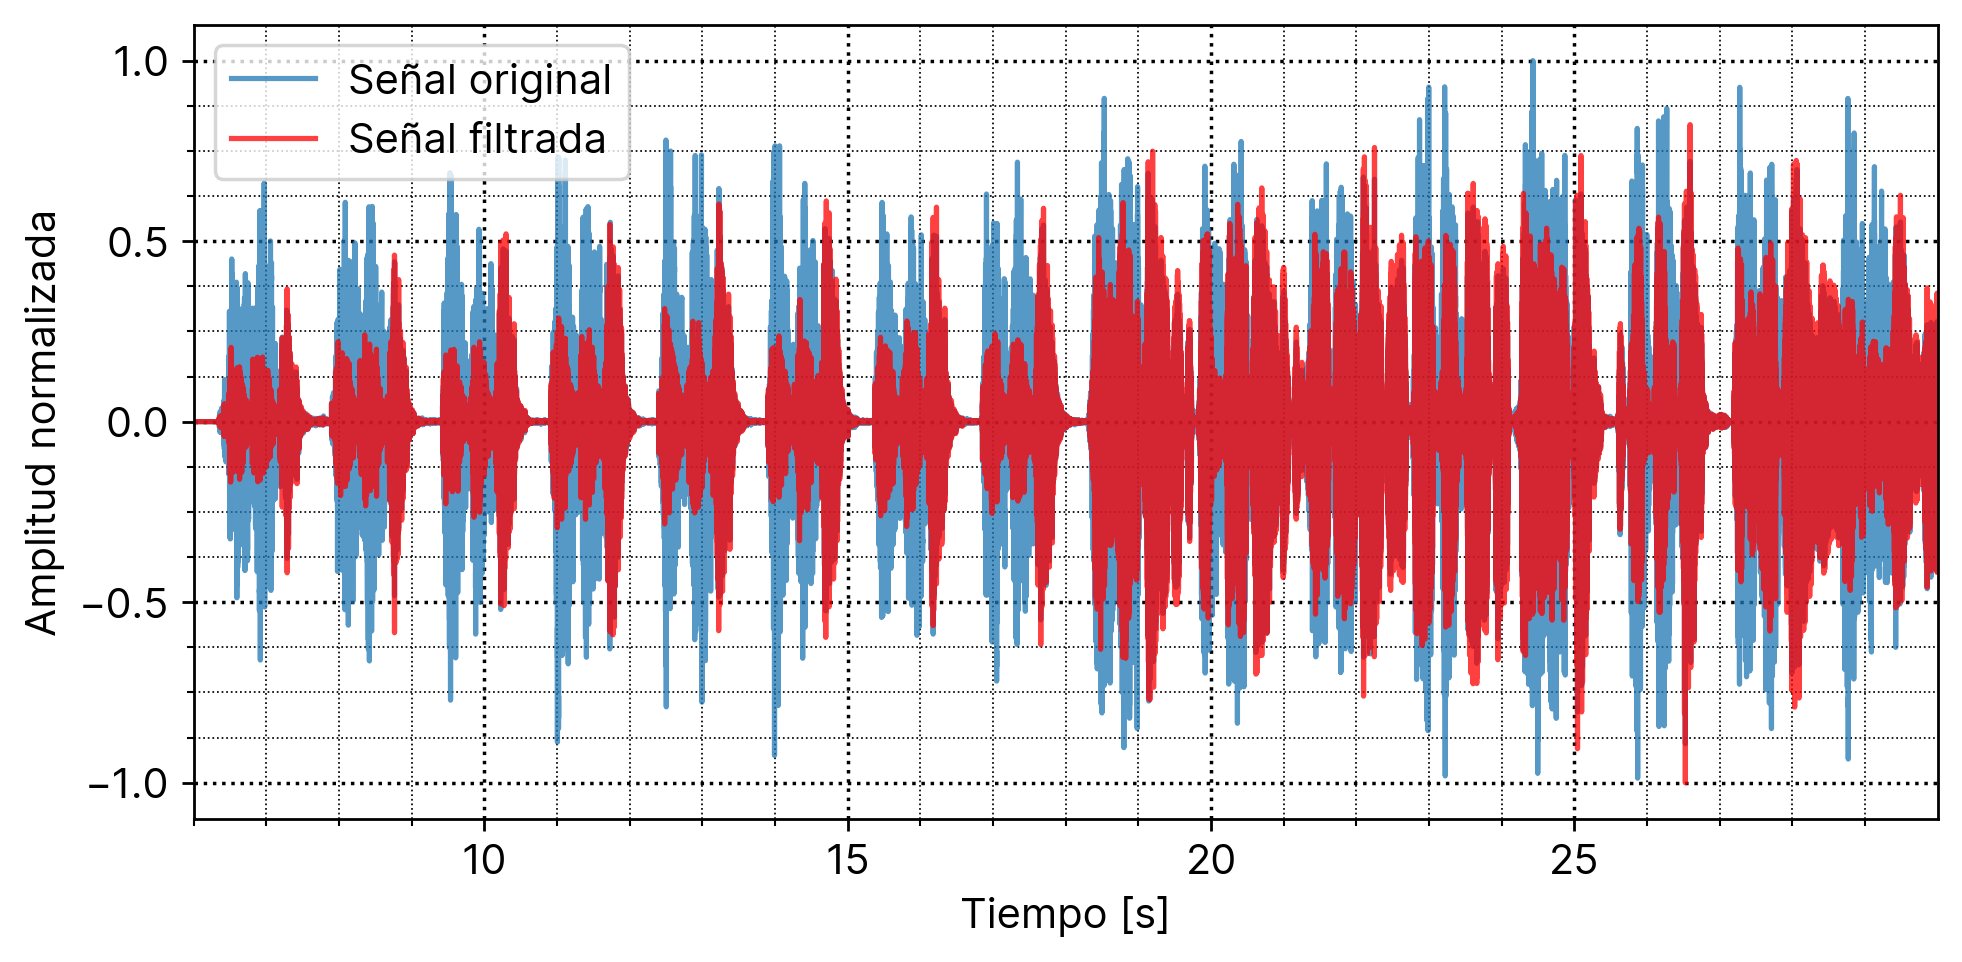
\includegraphics{plot/cancion2_6s_filter1_output_compare.png}
\caption{Segunda muestra salida de filtro 1}
\label{cancion2_filter1_output_compare}
\end{figure}

\begin{figure}
\centering
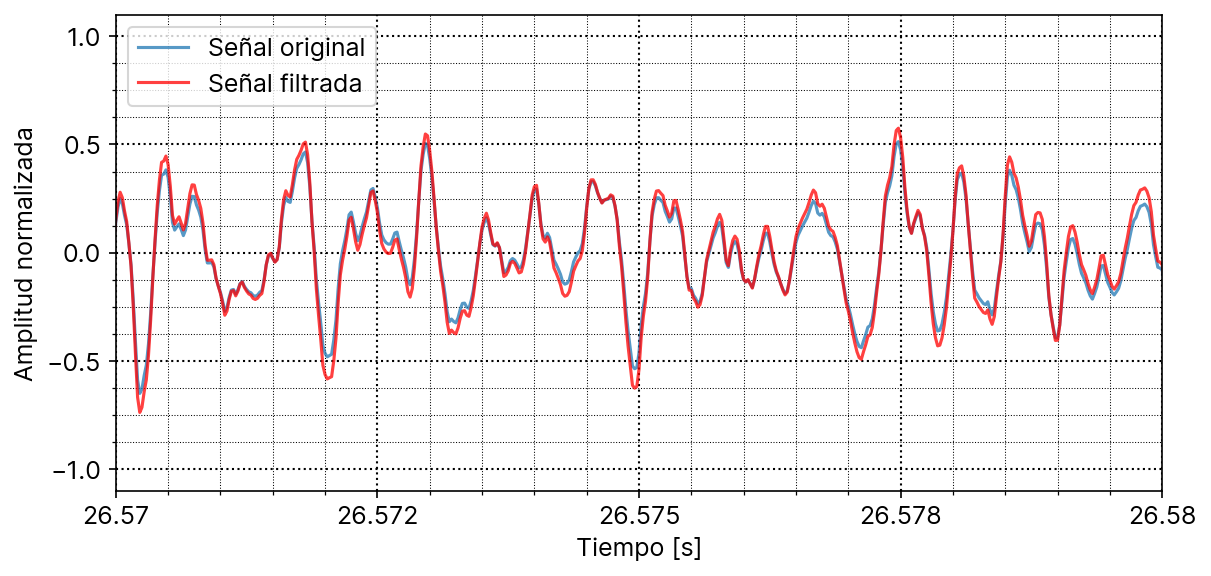
\includegraphics{plot/cancion2_6s_filter1_output_compare_26_57_a_26_58.png}
\caption{Segunda muestra salida de filtro 1 intervalo 26.57 a 26.58s}
\label{cancion2_6s_filter1_output_compare_26_57_a_26_58}
\end{figure}

\begin{figure}
\centering
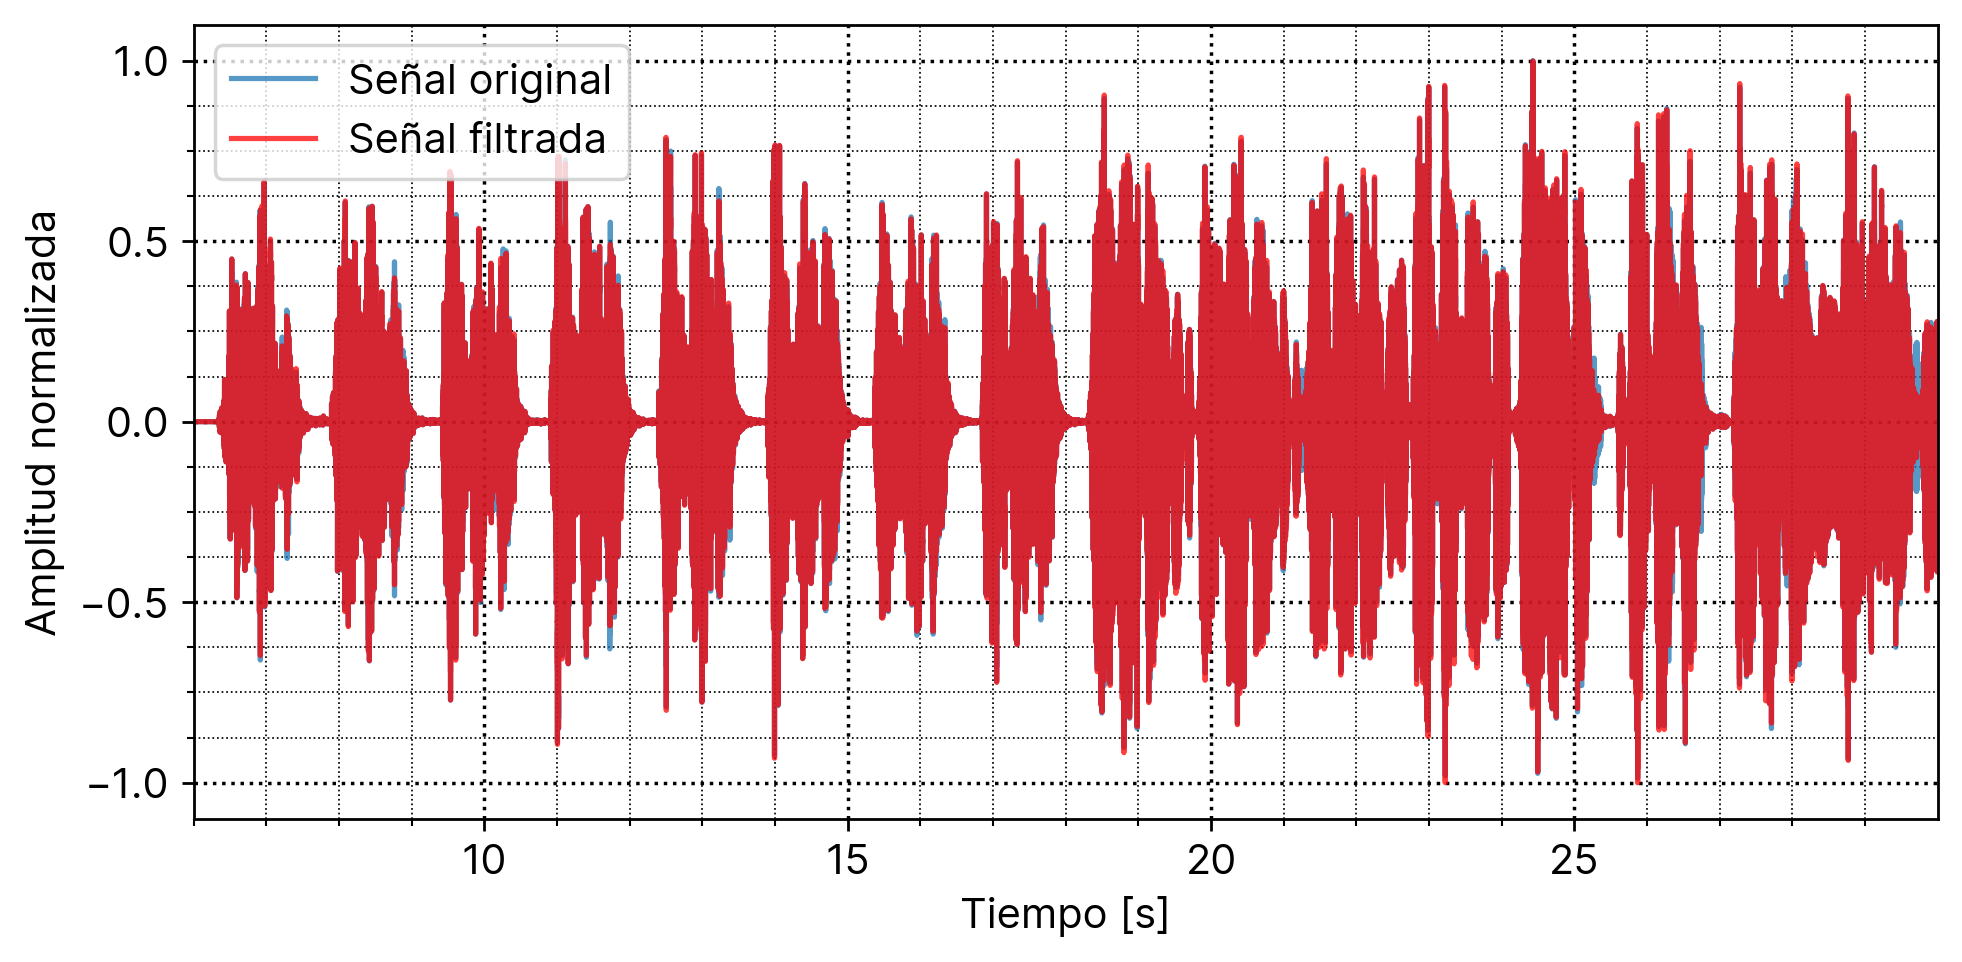
\includegraphics{plot/cancion2_6s_filter2_output_compare.png}
\caption{Segunda muestra salida de filtro 2}
\label{cancion2_filter2_output_compare}
\end{figure}

\begin{figure}
\centering
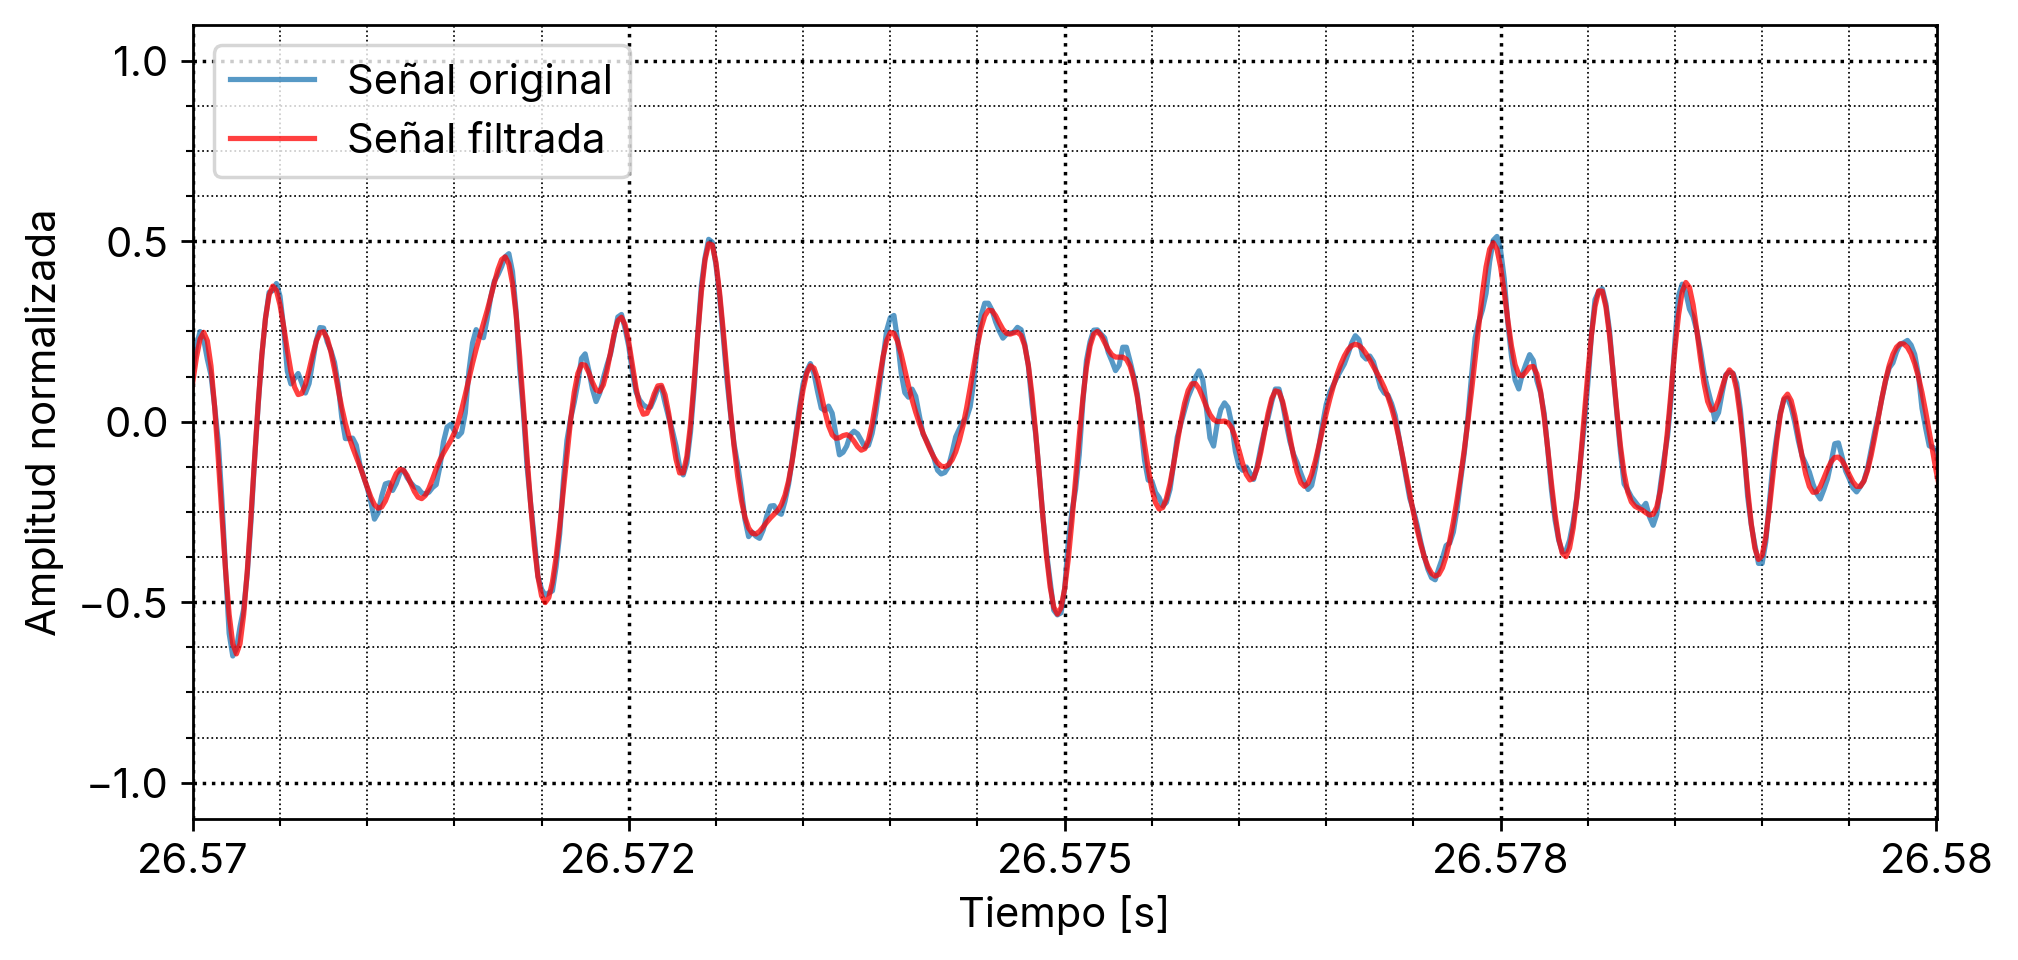
\includegraphics{plot/cancion2_6s_filter2_output_compare_26_57_a_26_58.png}
\caption{Seguida muestra salida de filtro 2 intervalo 26.57 a 26.58s}
\label{cancion2_6s_filter2_output_compare_26_57_a_26_58}
\end{figure}


En las figura \ref{cancion2_filter2_output_compare} se muestra la señal completa
de la salida luego de aplicar el segundo filtro a la segunda muestra, de esta
figura no se pueden sacar grandes conclusiones mas que una leve atenuación de
toda la señal. Analizando en mayor detalle, por ejemplo el intervalo de 26.57 a
26.58 segundos, como se muestra en la figura
\ref{cancion2_6s_filter2_output_compare_26_57_a_26_58} se observa algo similar a
lo observado para la primer muestra luego de aplicar este filtro y es el
suavizado que realiza.

En todos los casos, tanto para la primer muestra como para la segunda y
tanto para el primer filtro como el segundo, escuchando la respectiva
salida se confirma lo analizado desde el punto de vista del gráfico de
la señal, pero ademas se aprecia que el primer filtro realiza una
atenuación de las frecuencias mas altas (sonidos agudos) mientras que el
segundo disminuye las frecuencias bajas (o sonidos graves) esto ultimo
no se aprecia en el gráfico de la señal, ya que parece no tener efecto
mas que une leve atenuación.

\hypertarget{sonido-de-diferentes-instrumentos}{%
\subsection{Sonido de diferentes
instrumentos}\label{sonido-de-diferentes-instrumentos}}

Se generaron tres muestras diferentes a las ya utilizadas, correspondientes con
la nota \emph{A4} (La4, \(440\) Hz) mediante la simulación de tres instrumentos
musicales distintos: un clarinete, una flauta y un violín. Las señales generadas
corresponden con los archivos a4\_clarinete.wav, a4\_flauta.wav y a4\_violin.wav
y los gráficos de cada señal se muestran en las figuras 11, 12 y 13,
respectivamente.

Si bien todos los sonidos tienen la misma frecuencia, ya que es la misma
nota musical, el sonido escuchado percibido es diferente, esto puede ser
producto de la forma de onda generada por cada instrumento, lo cual
queda clara la diferencia en los respectivos gráficos.

Cada sonido percibido tiene características diferentes, el mas apagado o
neutro es el producido por la flauta, mientras que el mas agudo o
``afilado'' es el producido por el violín, el sonido del clarinete es un
intermedio entre ambos, un sonido ni muy agudo ni muy grave o apagado, y
con cierto carácter metálico.

Para el caso del clarinete, cuya señal se puede ver en la figura 11 a
continuación se puede ver que la onda se parece a una onda cuadrada. En
el dominio de frecuencia, las ondas cuadradas ideales se componen de
armónicos impares.

\begin{figure}
\centering
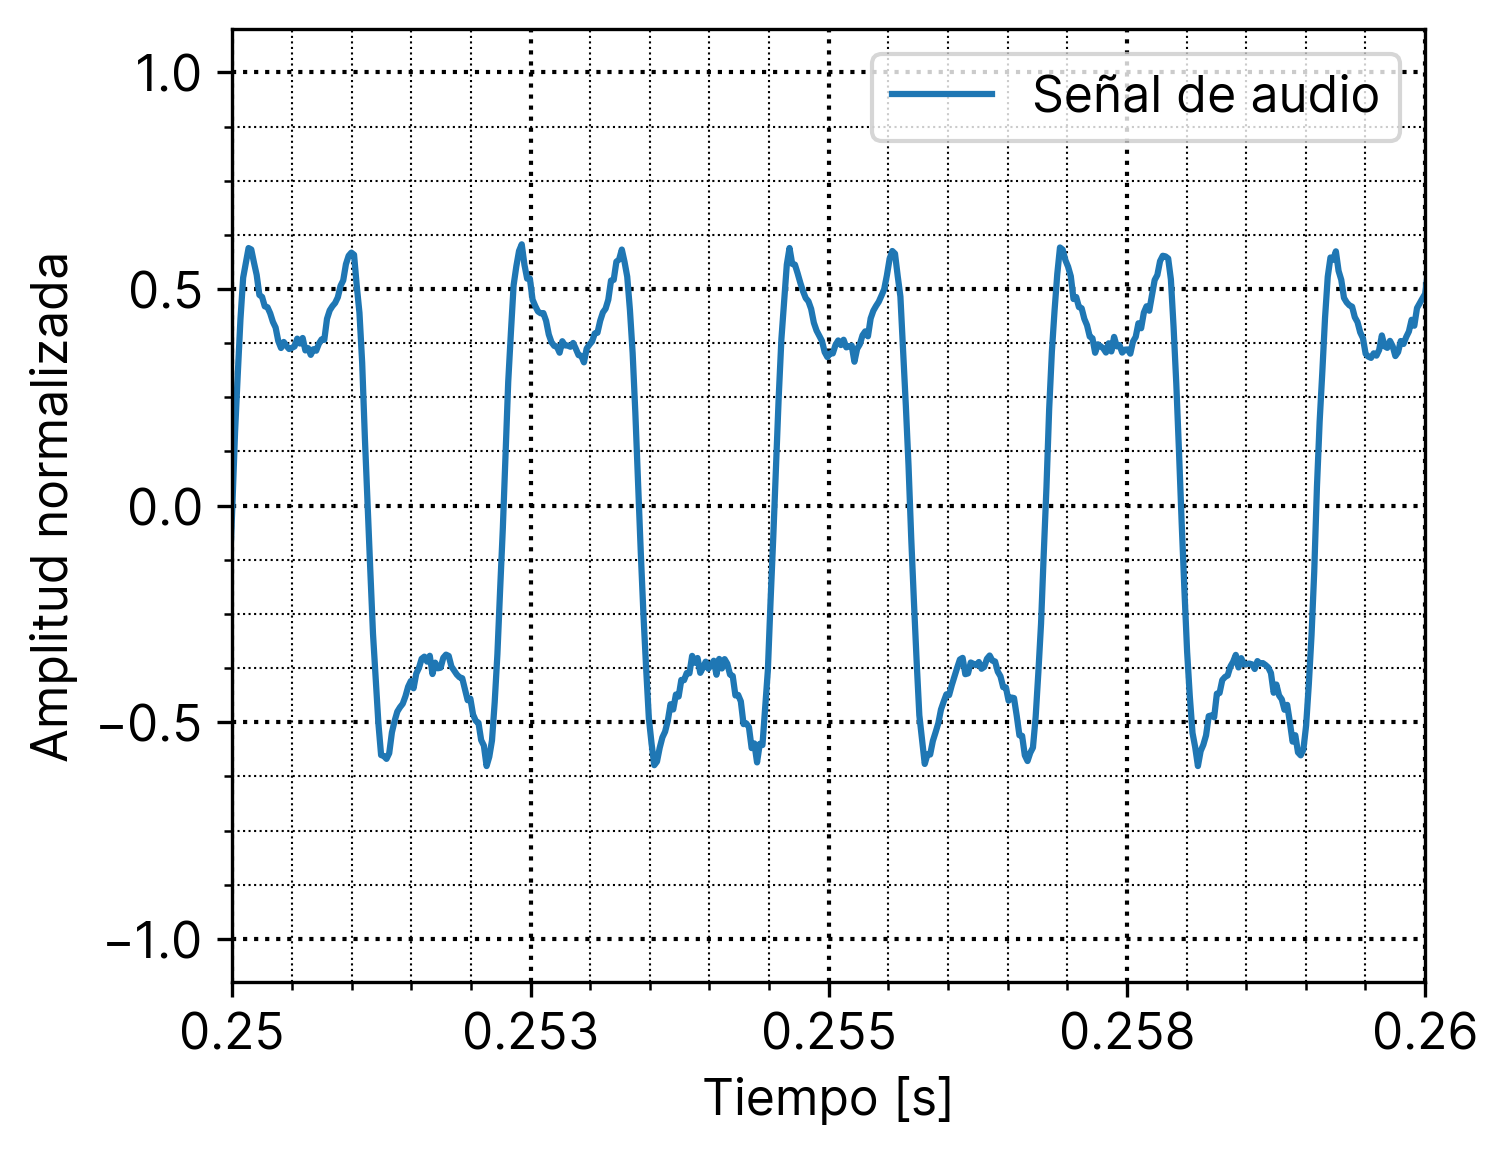
\includegraphics{plot/a4_clarinete.png}
\caption{Sonido de clarinete}
\label{a4_clarinete}
\end{figure}

Para la señal producida por la flauta que se puede ver en la figura 12,
se puede ver que se asemeja a una señal senoidal pura, aunque no tan
simétrica en los picos, las ondas sinodales en el dominio de frecuencia
tienen un único armónico, y es el fundamental, es por esto que el sonido
es mas neutro y no tan ``brillante'' o agudo dado que la frecuencia es
la misma en todos los casos.

\begin{figure}
\centering
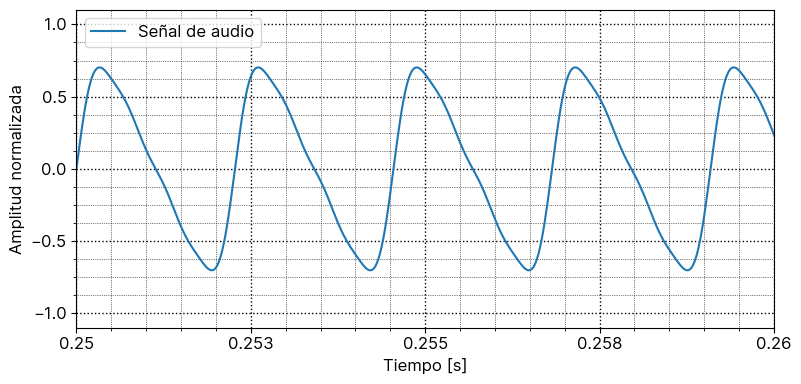
\includegraphics{plot/a4_flauta.png}
\caption{Sonido de flauta}
\label{a4_flauta}
\end{figure}

Por ultimo para la señal producida por el violín, la cual se puede ver
en la figura 13, se asemeja a una onda triangular con pendiente
decreciente, estas ondas triangulares en el dominio de frecuencia
también tienen armónicos impares como la onda cuadrada, pero estos
armónicos tienen mayor amplitud, es por esto que si bien tienen un
sonido similar, el sonido del violín es mas agudo.

\begin{figure}
\centering
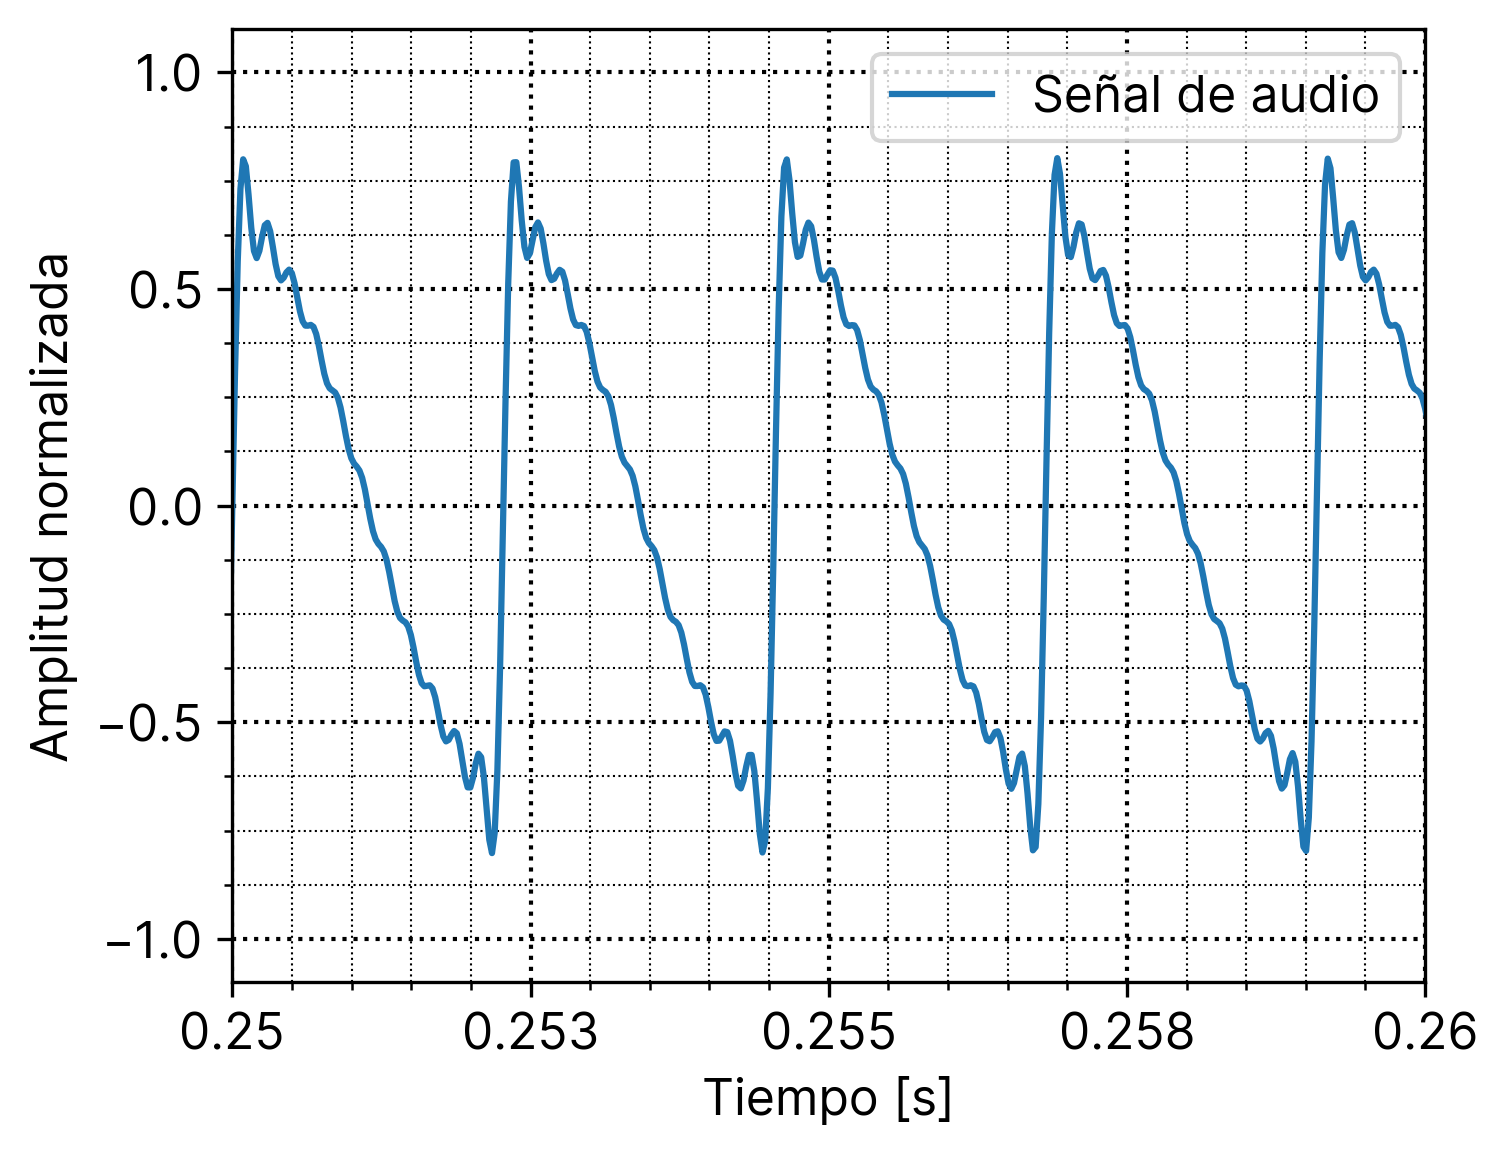
\includegraphics{plot/a4_violin.png}
\caption{Sonido de violín}
\label{a4_violin}
\end{figure}









\hypertarget{Dominio-de-frecuencia}{%
\section{Dominio de frecuencia}\label{dominio-de-frecuencia}}

En esta sección se analizan las mismas señales de audio que en la
sección anterior, correspondientes a los archivos cancion1.wav y cancion2.wav, pero en el dominio de la frecuencia. Para esto se calcula la
transformada discreta de fourier (DFT) de las mismas mediante un script de
Python (que internamente utiliza el algoritmo FFT). El resultado se muestra en
los figuras \ref{cancion1_fft} y \ref{cancion2_fft} para la señal de audio de
las canciones 1 y 2 respectivamente.

Se puede ver en la figura \ref{cancion1_fft} correspondiente a la primer canción
picos angostos en frecuencias determinadas, en cambio para la segunda canción en
la figura \ref{cancion2_fft}, se puede ver que la energía se distribuye en mas
frecuencias ya que los picos no están tan definidos. Esto puede deberse a que en
la primer canción se hallaban porciones periódicas de la señal en el dominio
temporal mientras que para la segunda canción había mayor presencia de señales
no periódicas.

\begin{figure}[H]
\centering
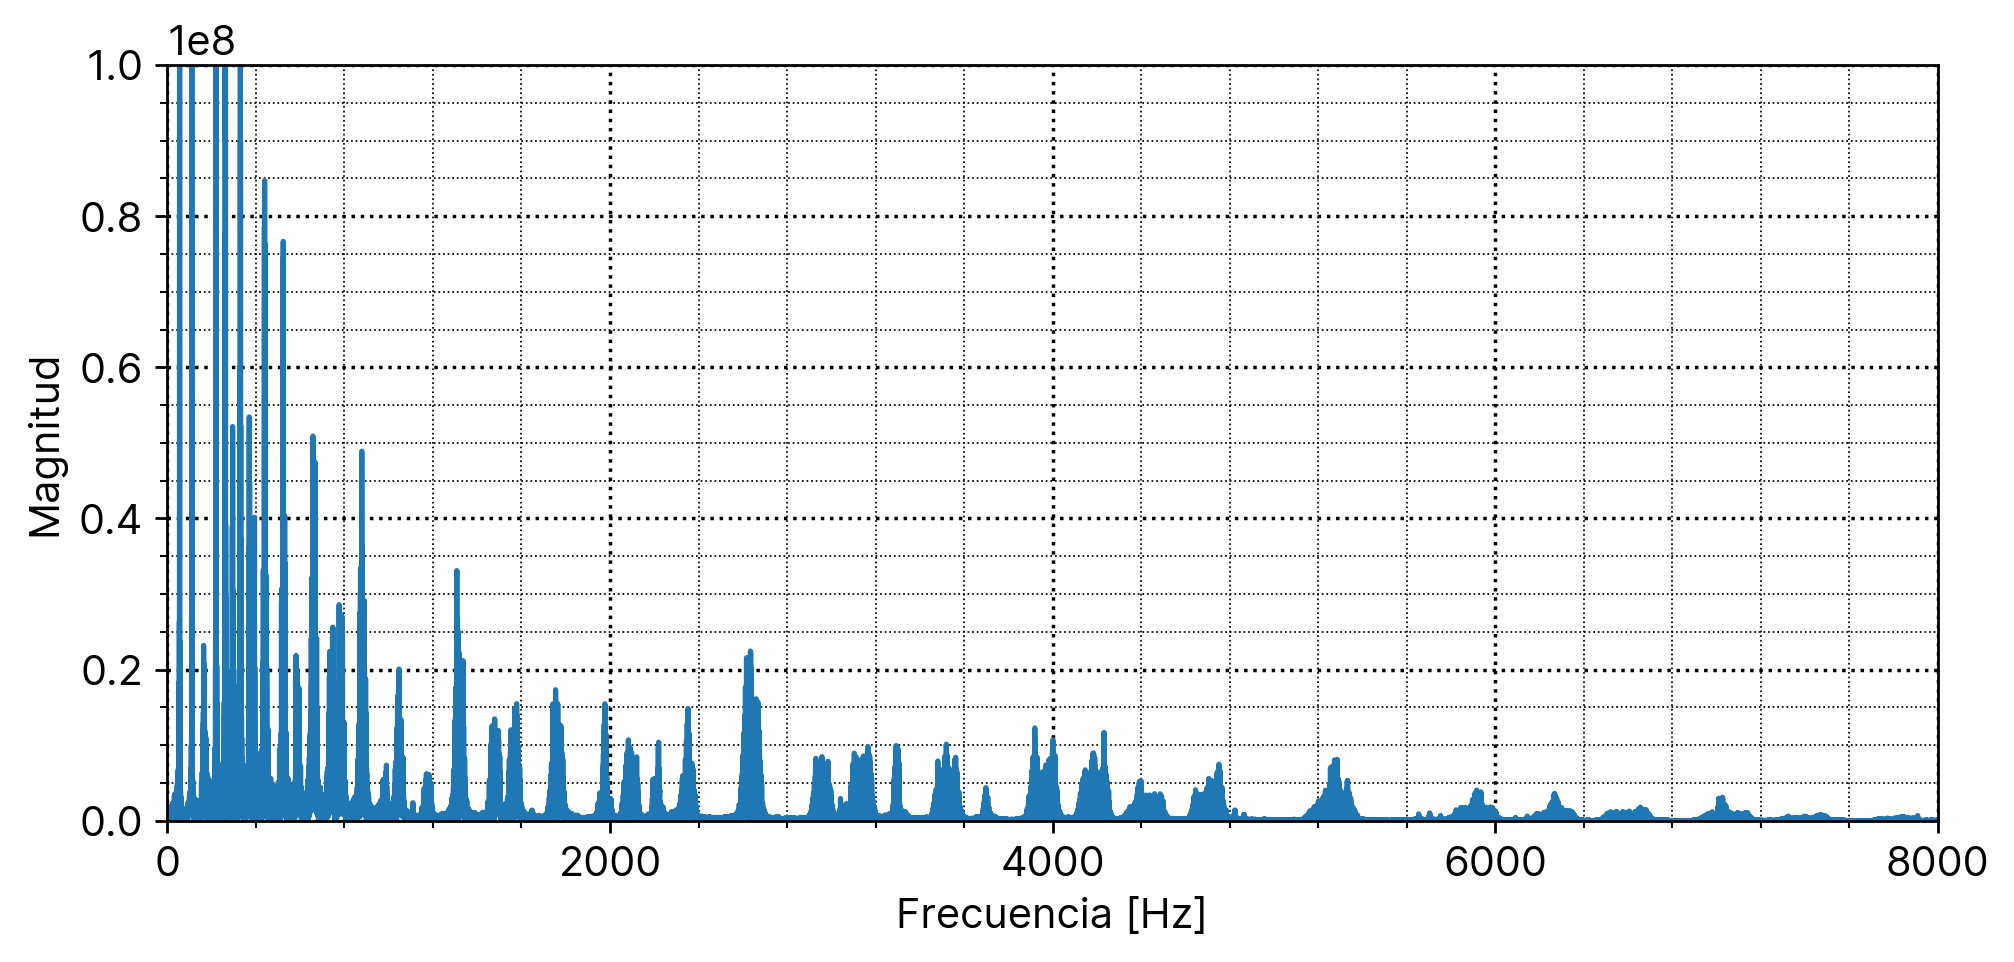
\includegraphics{plot/cancion1_fft.png}
\caption{Espectro de `cancion1.wav'}
\label{cancion1_fft}
\end{figure}

\begin{figure}[H]
\centering
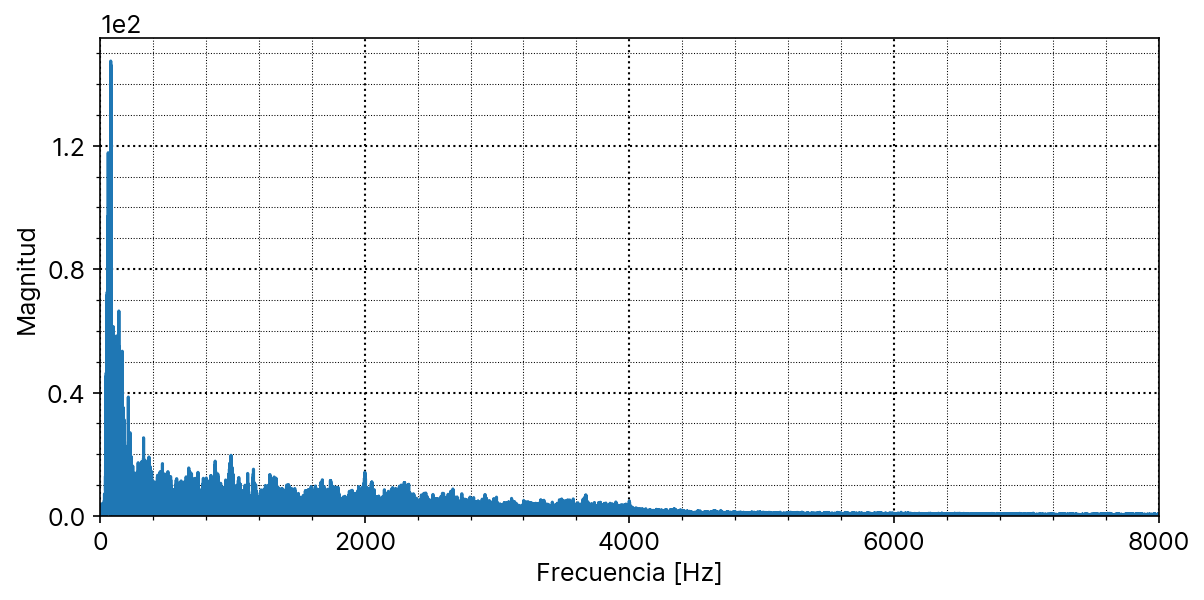
\includegraphics{plot/cancion2_fft.png}
\caption{Espectro de `cancion2.wav'}
\label{cancion2_fft}
\end{figure}

\hypertarget{filtrado}{%
\subsection{Filtrado}\label{filtrado}}

A continuación se utilizaron las señales filtradas obtenidas en la primera parte y se graficaron sus espectros en frecuencia, como se puede observar en las figuras \ref{cancion1_filter1_output_fft}, \ref{cancion1_filter2_output_fft}, \ref{cancion2_filter1_output_fft} y \ref{cancion2_filter2_output_fft}. Los gráficos \ref{filter1_h_fft} y \ref{filter2_h_fft} corresponden a las transformadas de Fourier de los filtros utilizados anteriormente.

\begin{figure}[H]
\centering
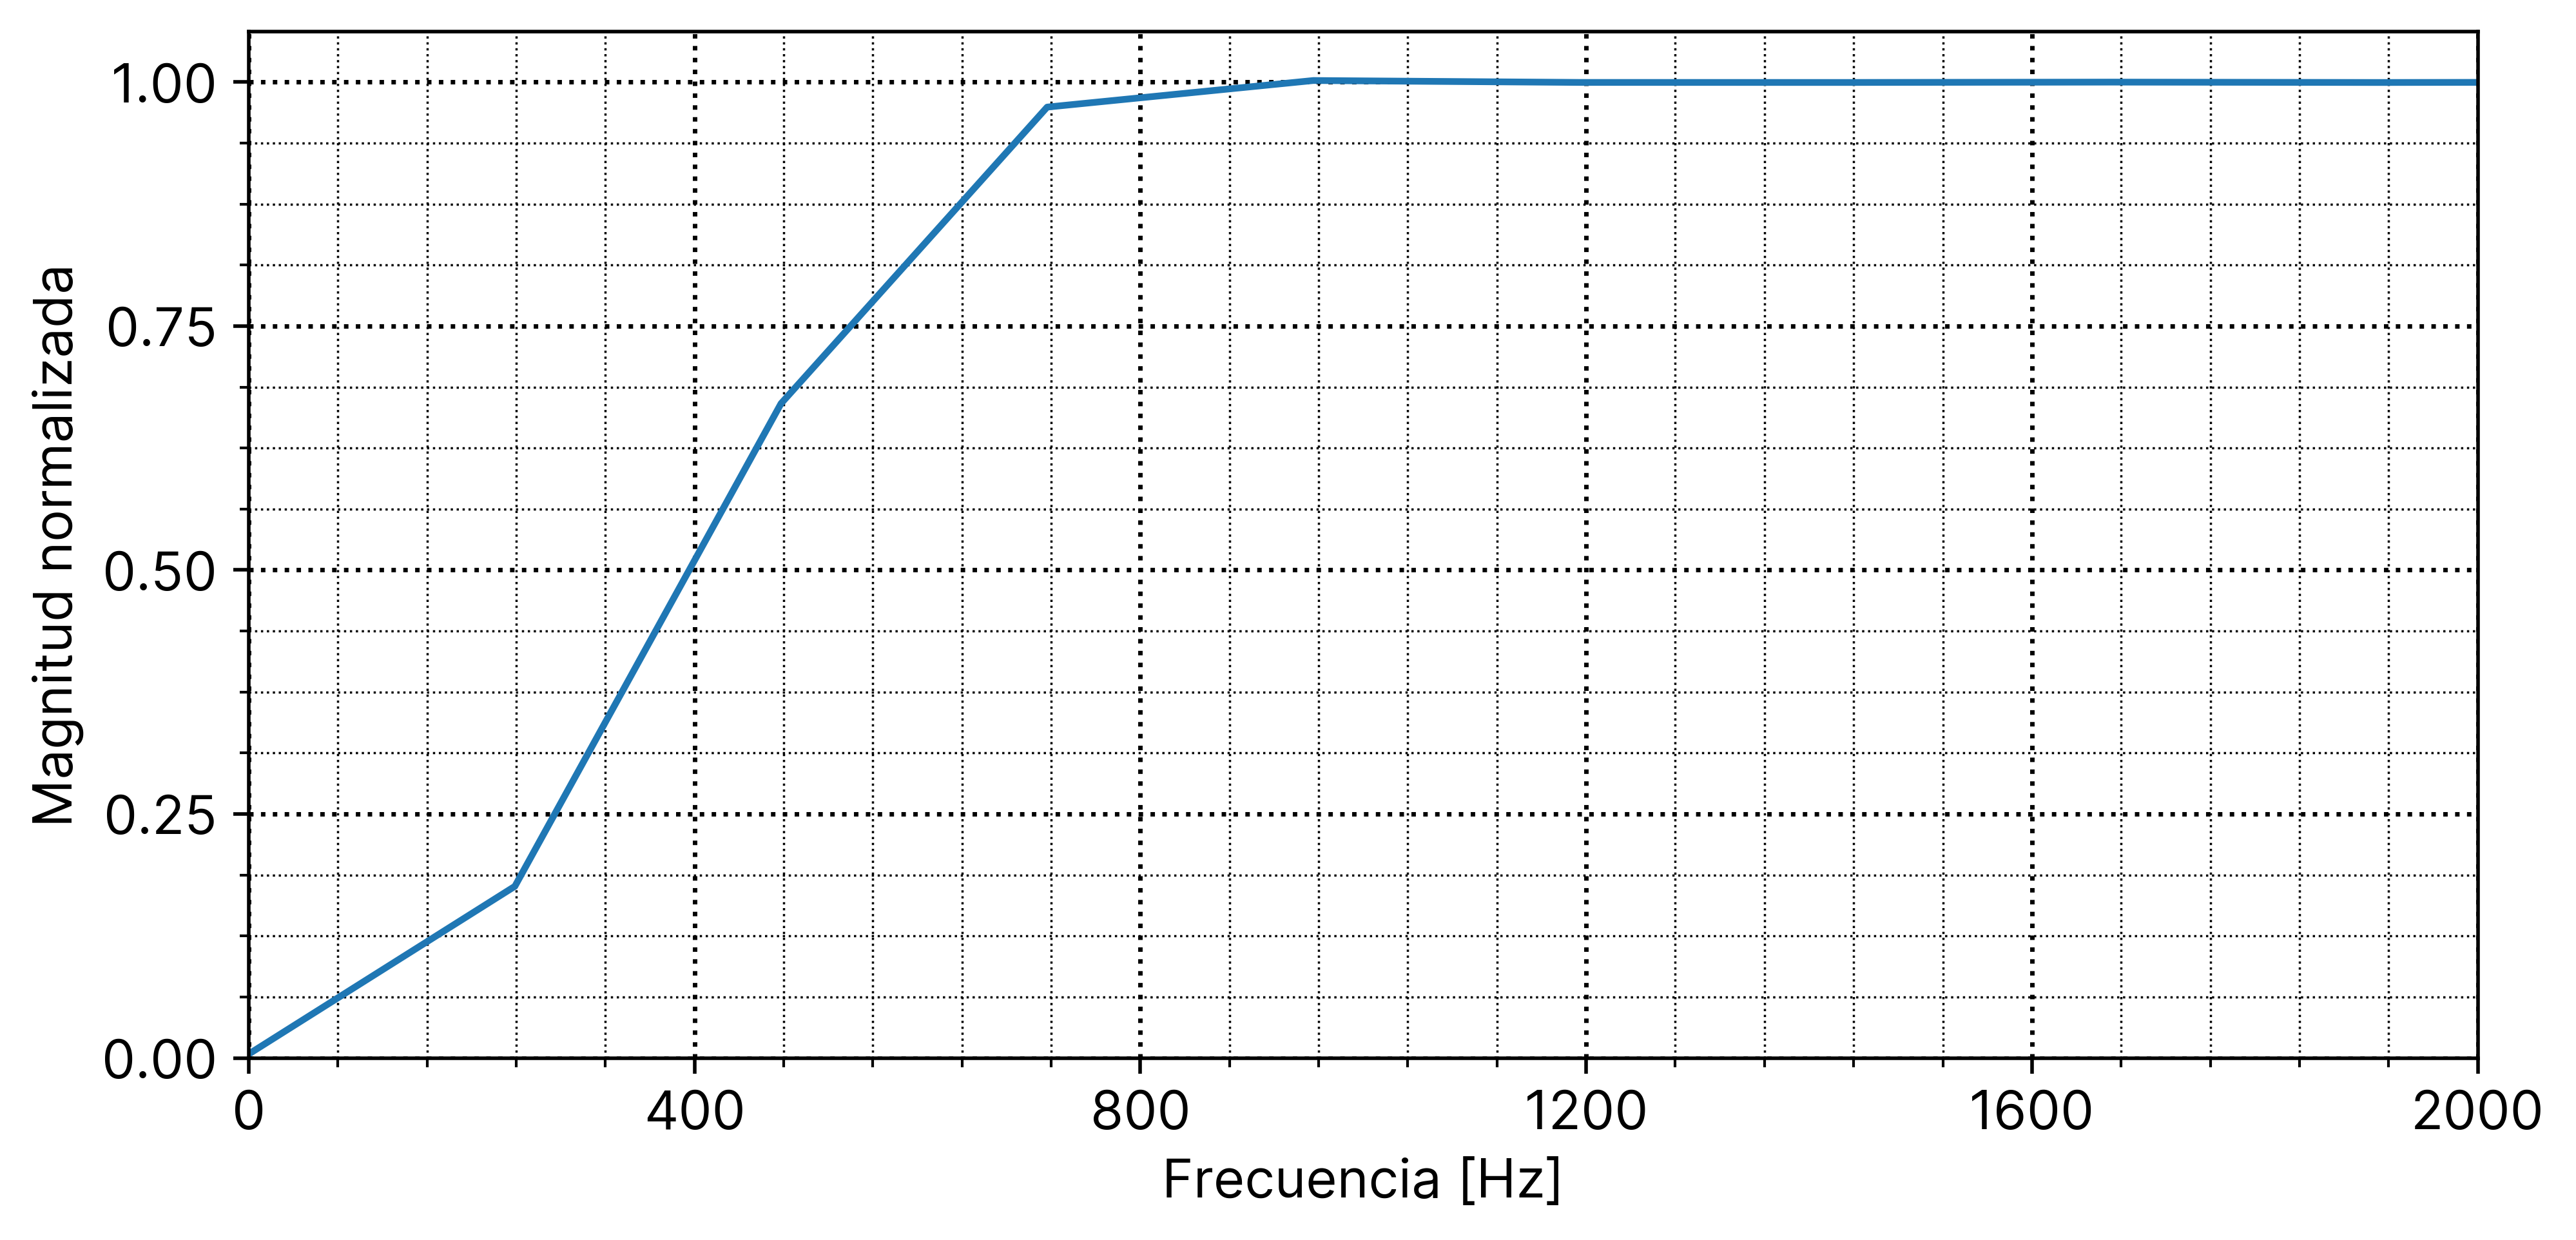
\includegraphics{plot/filter1_h_fft.png}
\caption{Transformada de Fourier del primer filtro}
\label{filter1_h_fft}
\end{figure}

\begin{figure}[H]
\centering
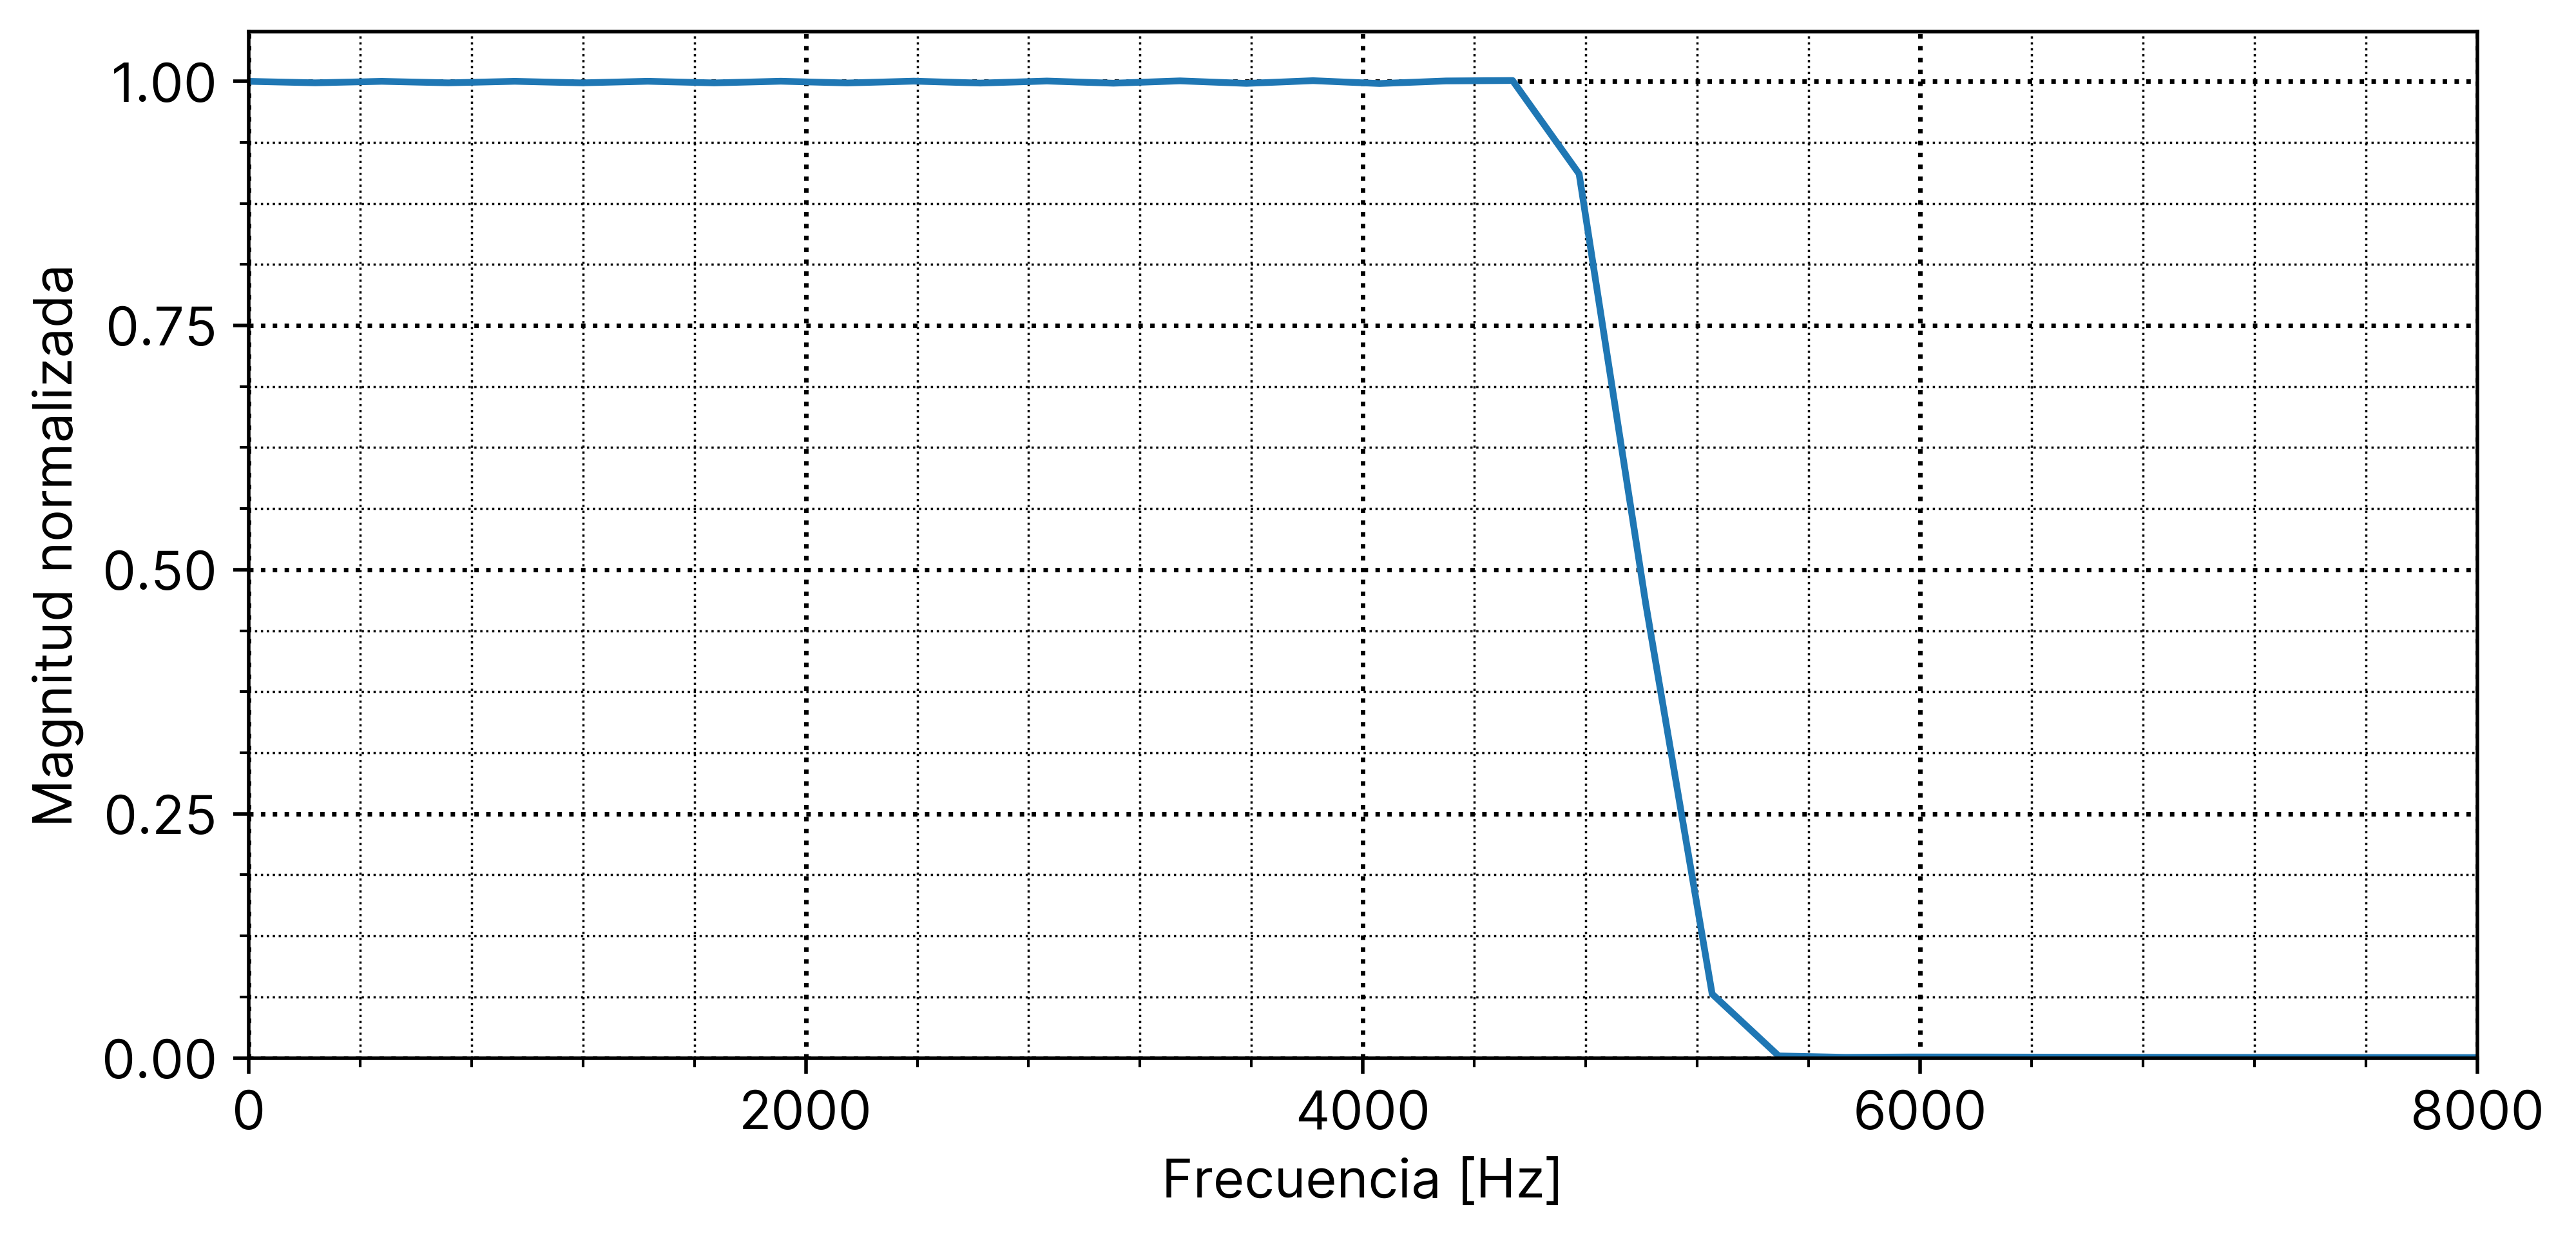
\includegraphics{plot/filter2_h_fft.png}
\caption{Transformada de Fourier del segundo filtro}
\label{filter2_h_fft}
\end{figure}

Como era de esperarse y como se anticipó en la primera parte, el primer filtro corresponde a un filtro pasa altos mientras que el segundo es un filtro pasa bajos. En el caso del primero deja pasar por completo las frecuencias mayores a 800Hz aproximadamente y atenua en mayor o menor medida las frecuencias restantes, mientras que el segundo deja pasar las frecuencias menores a 4600Hz aproximadamente, atenua por completo las frecuencias mayores a 5600Hz aproximadamente y atenua en mayor o menor medida las que están en el medio.

\begin{figure}[H]
\centering
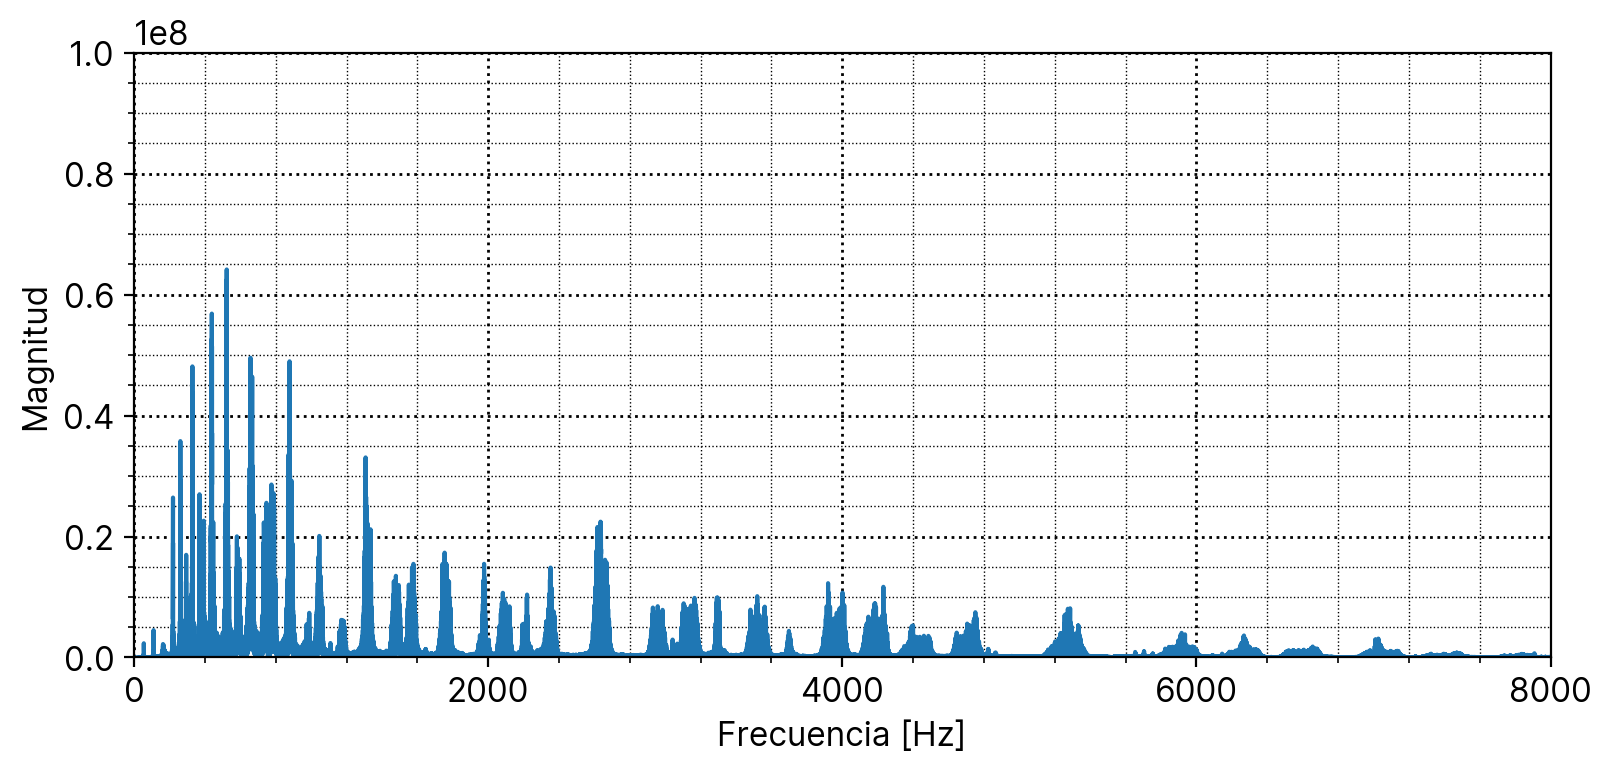
\includegraphics{plot/cancion1_filter1_output_fft.png}
\caption{Espectro de `cancion1.wav' con filtro 1 aplicado}
\label{cancion1_filter1_output_fft}
\end{figure}

\begin{figure}[H]
\centering
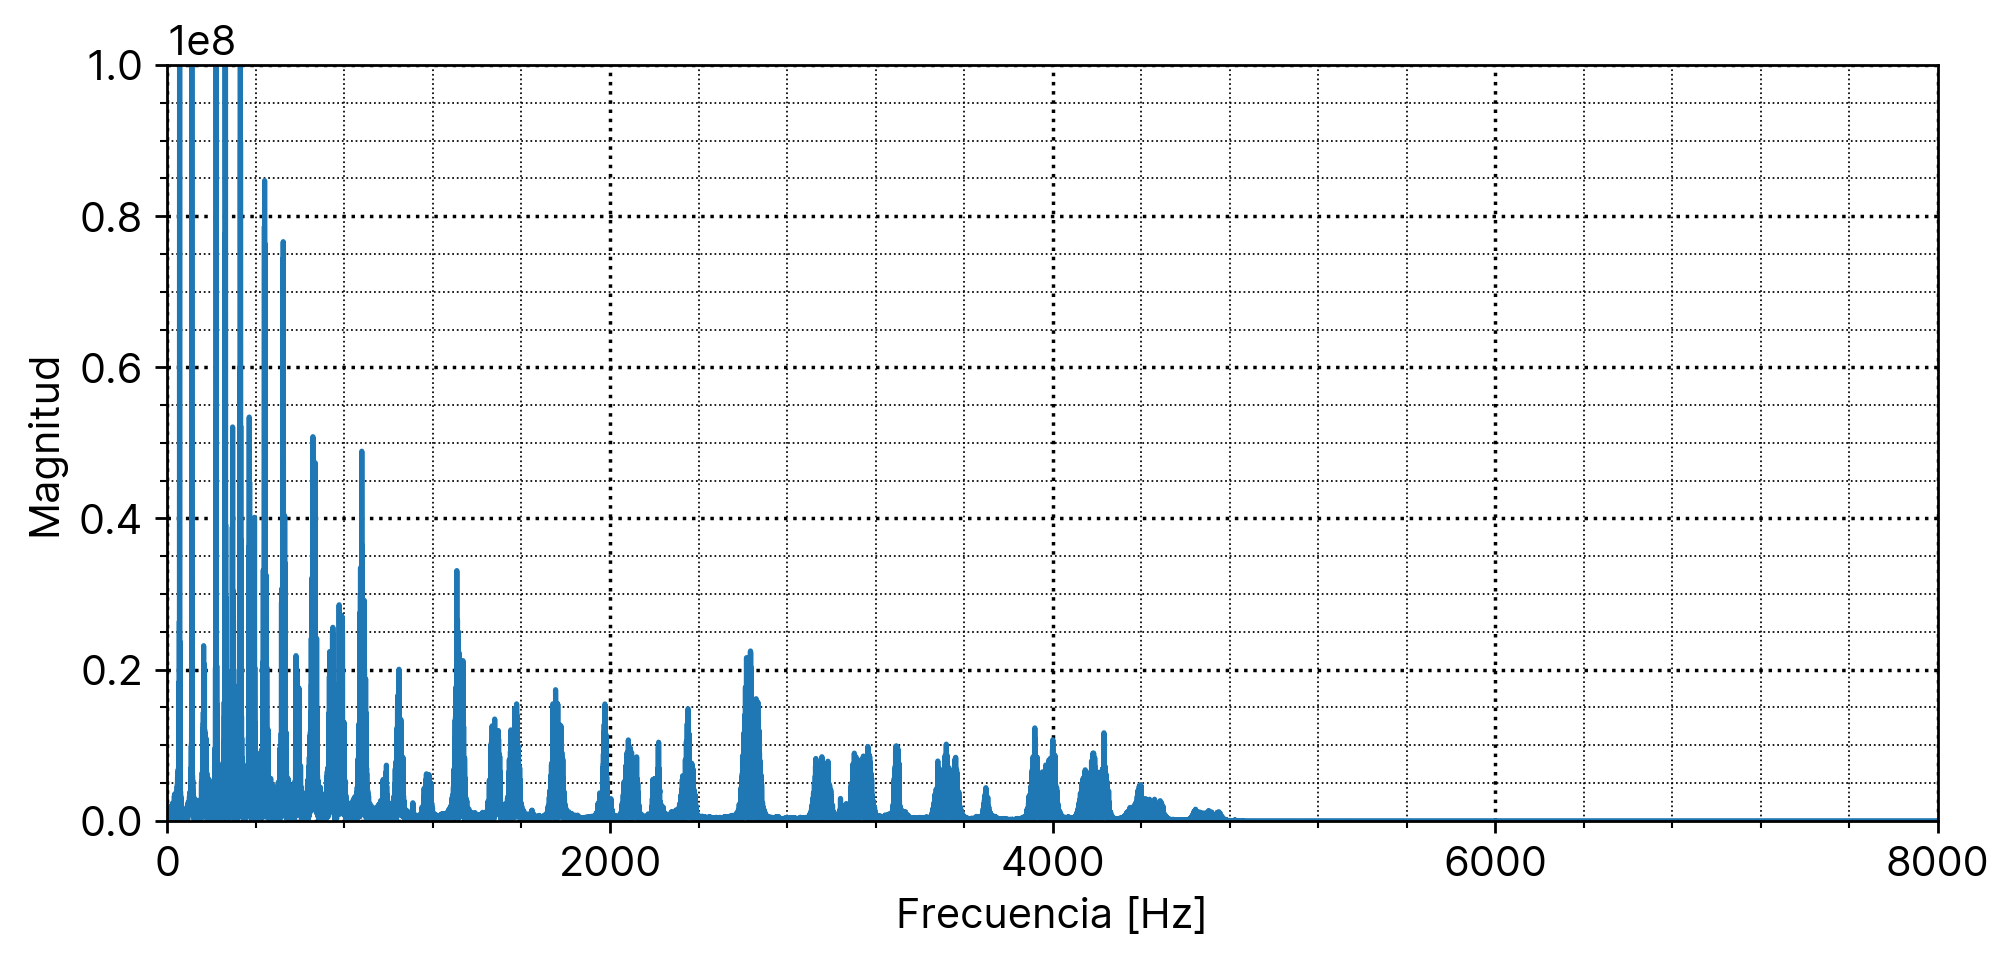
\includegraphics{plot/cancion1_filter2_output_fft.png}
\caption{Espectro de `cancion1.wav' con filtro 2 aplicado}
\label{cancion1_filter2_output_fft}
\end{figure}

\begin{figure}[H]
\centering
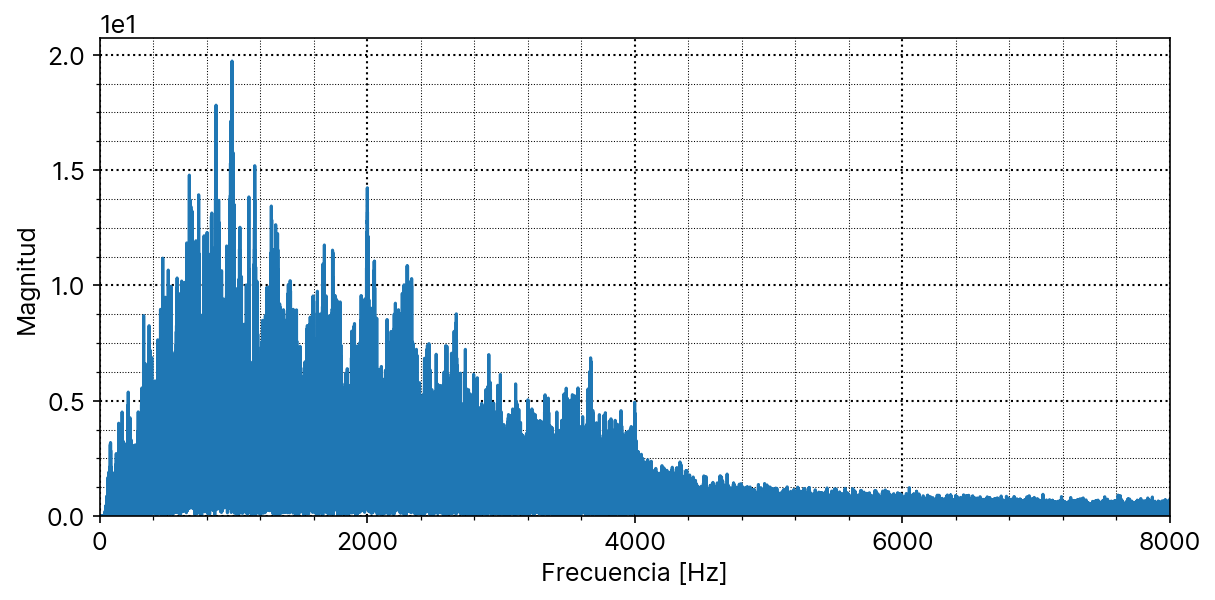
\includegraphics{plot/cancion2_filter1_output_fft.png}
\caption{Espectro de `cancion2.wav' con filtro 1 aplicado}
\label{cancion2_filter1_output_fft}
\end{figure}

\begin{figure}[H]
\centering
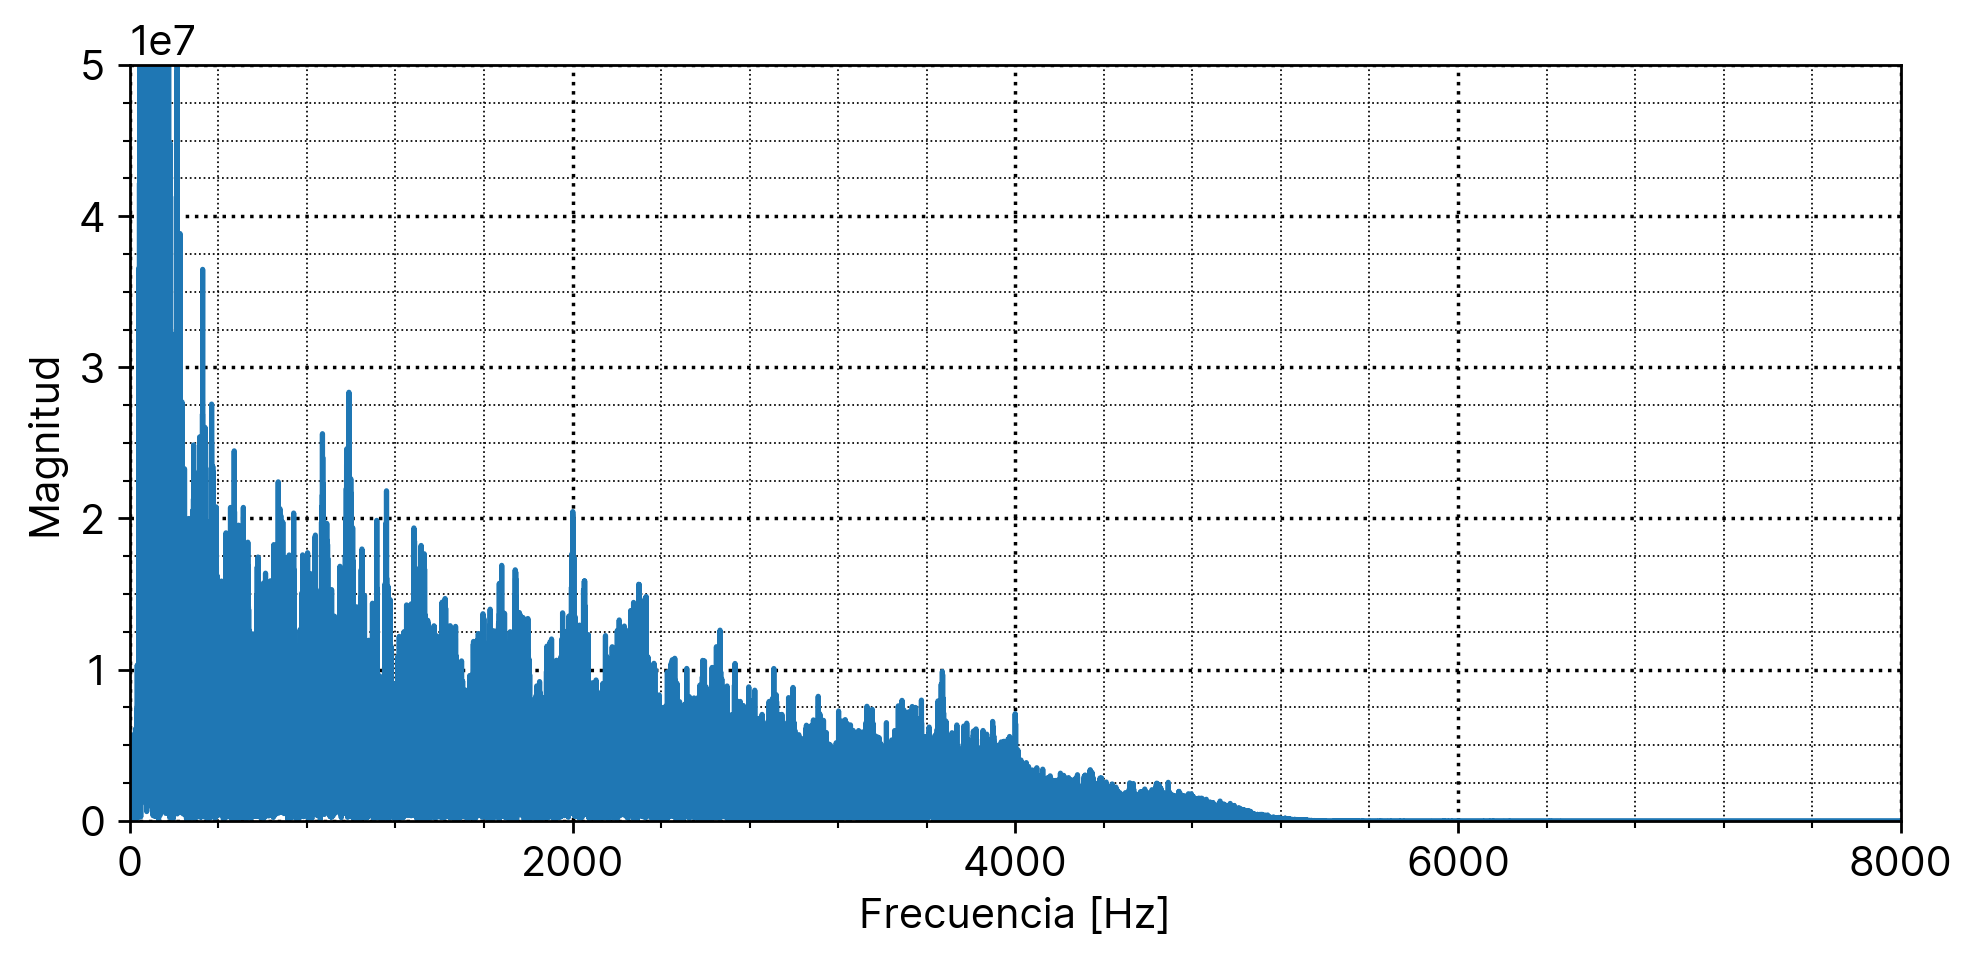
\includegraphics{plot/cancion2_filter2_output_fft.png}
\caption{Espectro de `cancion2.wav' con filtro 2 aplicado}
\label{cancion2_filter2_output_fft}
\end{figure}

Una de las formas de verificar si el sistema es LTI es con la siguiente relación:

\[
y(t) = (h * x)(t) = \int_{-\infty}^{\infty} h(\tau)\, x(t - \tau)\, d\tau
\]

ya que la salida $y(t)$ está dada por la convolución entre la señal de entrada $x(t)$ y la respuesta al impulso del sistema $h(t)$, al aplicar la transformada de Fourier a ambos lados de la ecuación, y utilizando la propiedad de que la convolución en el dominio del tiempo se convierte en una multiplicación en el dominio de la frecuencia, se obtiene:

\[
Y(\omega) = H(\omega) \cdot X(\omega)
\]

donde $X(\omega)$, $Y(\omega)$ y $H(\omega)$ son las transformadas de Fourier de $x(t)$, $y(t)$ y $h(t)$, respectivamente. Por lo tanto, si existe una función $H(\omega)$ tal que para una señal arbitraria $x(t)$ se cumple:

\[
Y(\omega) = H(\omega)\, X(\omega),
\]

entonces el sistema puede describirse completamente mediante su respuesta al impulso $h(t)$, y se concluye que es un sistema \textbf{lineal e invariante en el tiempo (LTI)}.

En cambio, si la relación entre $X(\omega)$ e $Y(\omega)$ no puede expresarse como una multiplicación por una función fija $H(\omega)$, esto indica que el sistema no es LTI, ya sea porque es no lineal o porque su comportamiento varía en el tiempo.

Por lo tanto, de forma manual se tomaron valores a una determinada frecuencia para ver si cumplen con esta relación. 


\hypertarget{espectogramas}{%
\subsection{Espectrogramas}\label{espectogramas}}

Un espectrograma es una representación de la transformada de Fourier en el tiempo, esto es una representación en tres dimensiones, pero en un plano con colores, en el eje X se representa el tiempo, en el eje Y se representa la frecuencia y el que seria el eje Z, saliente de la pantalla, en este caso representado por el color del pixel, se representa la magnitud del armónico.

Se tomaran diferentes longitudes de ventana, esto es la cantidad de muestras temporales que se toman de la señal para computar la DFT, un mayor numero implica mayor resolución en frecuencia pero menor resolución temporal, esto se manifiesta en el espectrograma por lineas o puntos bien definidos en el eje Y, pero difusos en las transiciones en el eje X, por el contrario un menor numero de puntos implica mayor resolución temporal pero menor resolución en frecuencia, esto es lineas o puntos cortantes en las transiciones en el eje X pero difusas en el eje Y.

\hypertarget{espectograma-ventana-rectangular}{%
\subsubsection{Espectrograma con ventana rectangular}\label{espectograma-ventana-rectangular}}

En las figuras \ref{cancion1_espectograma_boxcar_0512}, \ref{cancion1_espectograma_boxcar_1024} y \ref{cancion1_espectograma_boxcar_2048} se gráfica el espectrograma de la primer canción, utilizando una ventana rectangular en todos los casos, tomando 512, 1024 y 2048 puntos respectivamente.

\begin{figure}[H]
\centering
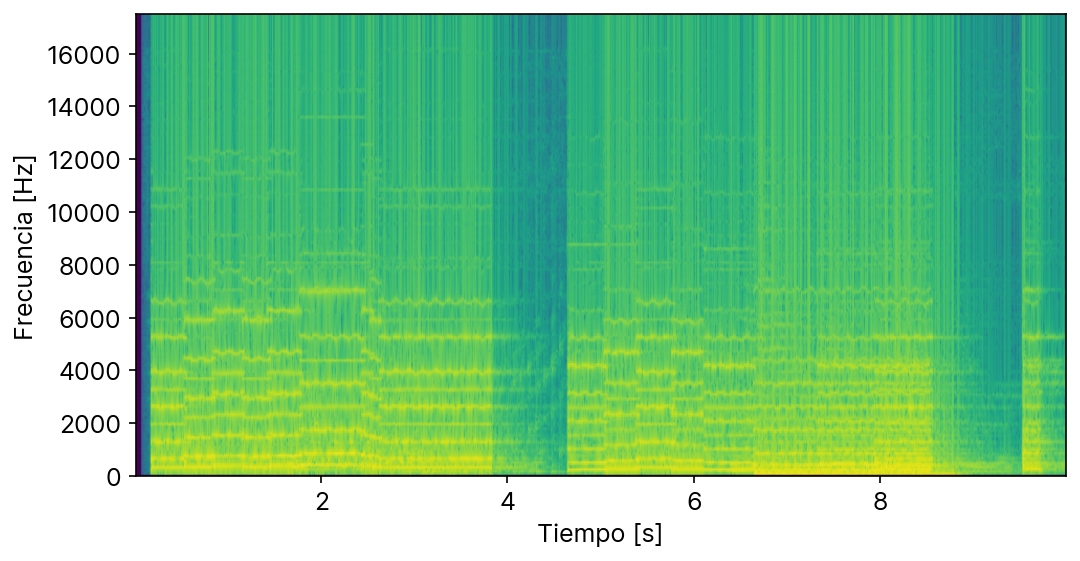
\includegraphics{plot/cancion1_espectograma_boxcar_0512.png}
\caption{Espectrograma primer muestra de ventana rectangular de 512 puntos}
\label{cancion1_espectograma_boxcar_0512}
\end{figure}

\begin{figure}[H]
\centering
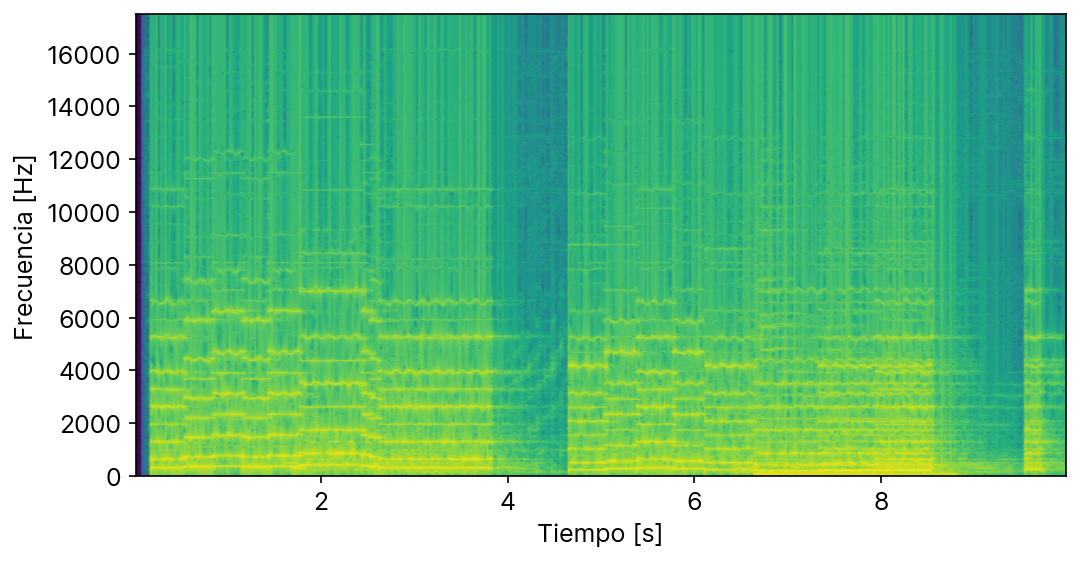
\includegraphics{plot/cancion1_espectograma_boxcar_1024.png}
\caption{Espectrograma primer muestra de ventana rectangular de 1024 puntos}
\label{cancion1_espectograma_boxcar_1024}
\end{figure}

\begin{figure}[H]
\centering
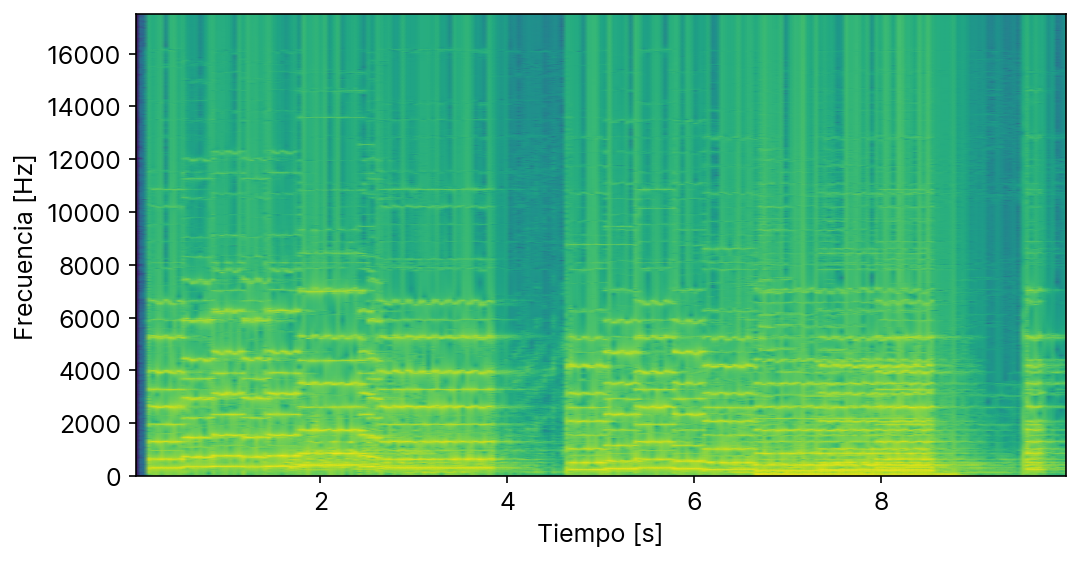
\includegraphics{plot/cancion1_espectograma_boxcar_2048.png}
\caption{Espectrograma primer muestra de ventana rectangular de 2048 puntos}
\label{cancion1_espectograma_boxcar_2048}
\end{figure}

De manera análoga, en las figuras \ref{cancion2_espectograma_boxcar_0512}, \ref{cancion2_espectograma_boxcar_1024} y \ref{cancion2_espectograma_boxcar_2048} se gráfica el espectrograma de la segunda canción, utilizando una ventana rectangular en todos los casos, tomando 512, 1024 y 2048 puntos respectivamente.

\begin{figure}[H]
\centering
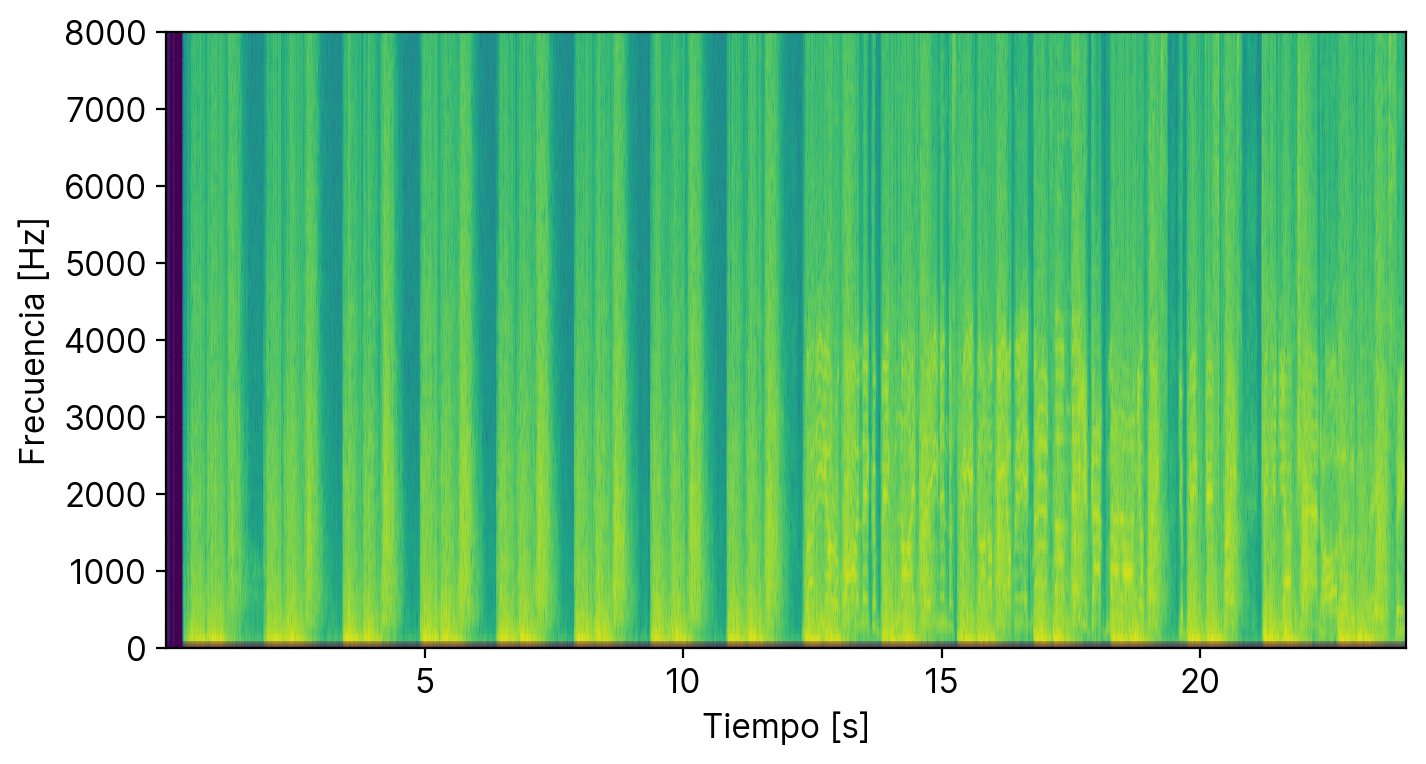
\includegraphics{plot/cancion2_espectograma_boxcar_0512.png}
\caption{Espectrograma segunda muestra de ventana rectangular de 512 puntos}
\label{cancion2_espectograma_boxcar_0512}
\end{figure}

\begin{figure}[H]
\centering
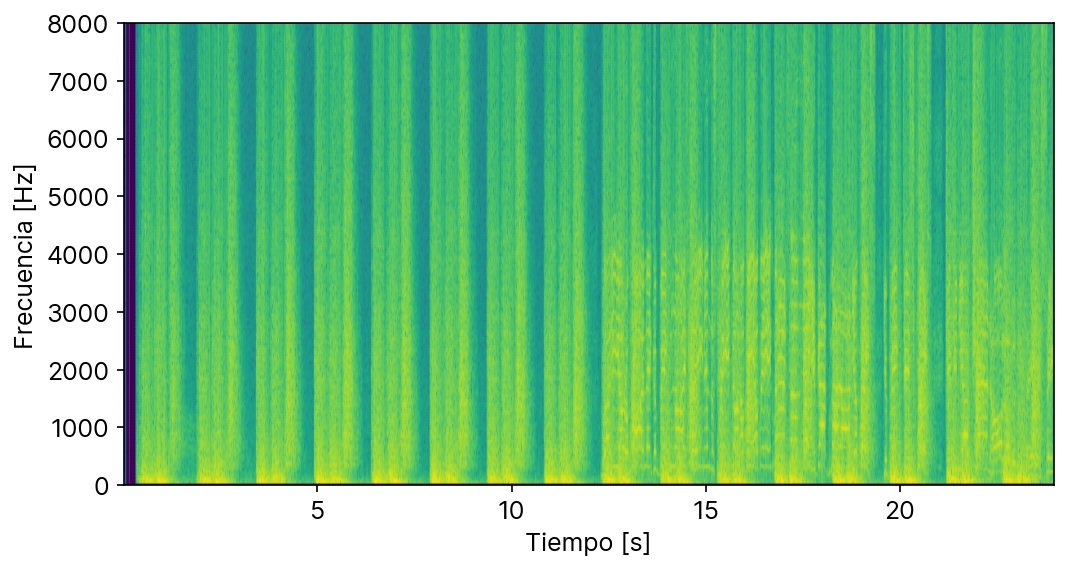
\includegraphics{plot/cancion2_espectograma_boxcar_1024.png}
\caption{Espectrograma segunda muestra de ventana rectangular de 1024 puntos}
\label{cancion2_espectograma_boxcar_1024}
\end{figure}

\begin{figure}[H]
\centering
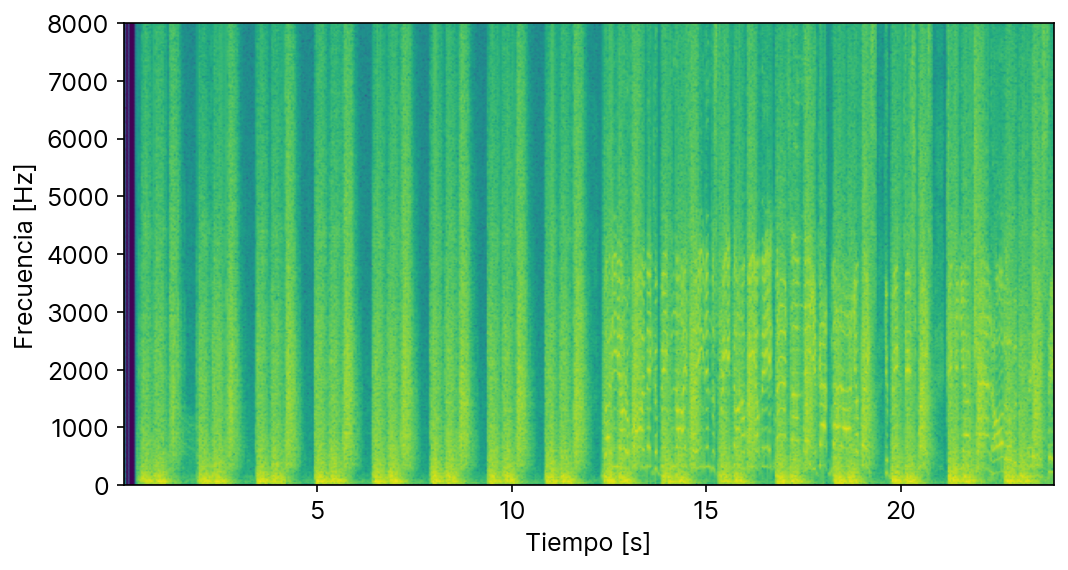
\includegraphics{plot/cancion2_espectograma_boxcar_2048.png}
\caption{Espectrograma segunda muestra de ventana rectangular de 2048 puntos}
\label{cancion2_espectograma_boxcar_2048}
\end{figure}

\hypertarget{espectograma-ventana-triangular}{%
\subsubsection{Espectrograma con ventana triangular}\label{espectograma-ventana-triangular}}

A continuación se vuelve a graficar los espectrogramas de las canciones 1 y 2 tomando la misma cantidad de puntos, 512, 1024 y 2048, pero la diferencia siendo que se utiliza una ventana triangular. La diferencia entre ambas ventanas en la practica es que la ventana rectangular tiene mejor resolución en frecuencia ya que su DFT es una función sinc (con la función sinc definida como $sin(\pi\cdot x)/\pi\cdot x$) pero mayor fuga espectral, ya que los lóbulos secundarios de las sinc son mas fuertes que la DFT de la función triangular, que es una sinc pero al cuadrado, lo que hace que los lóbulos secundarios disminuyan. Para la primer muestra las figuras resultantes son \ref{cancion1_espectograma_bartlett_0512}, \ref{cancion1_espectograma_bartlett_1024} y \ref{cancion1_espectograma_bartlett_2048}, para el espectrograma utilizando ventana triangular y tomando 512, 1024 y 2048 puntos respectivamente. Para la segunda muestra, las figuras resultantes son \ref{cancion2_espectograma_bartlett_0512}, \ref{cancion2_espectograma_bartlett_1024} y \ref{cancion2_espectograma_bartlett_2048} para el espectrograma utilizando ventana triangular y tomando 512, 1024 y 2048 puntos respectivamente.

\begin{figure}[H]
\centering
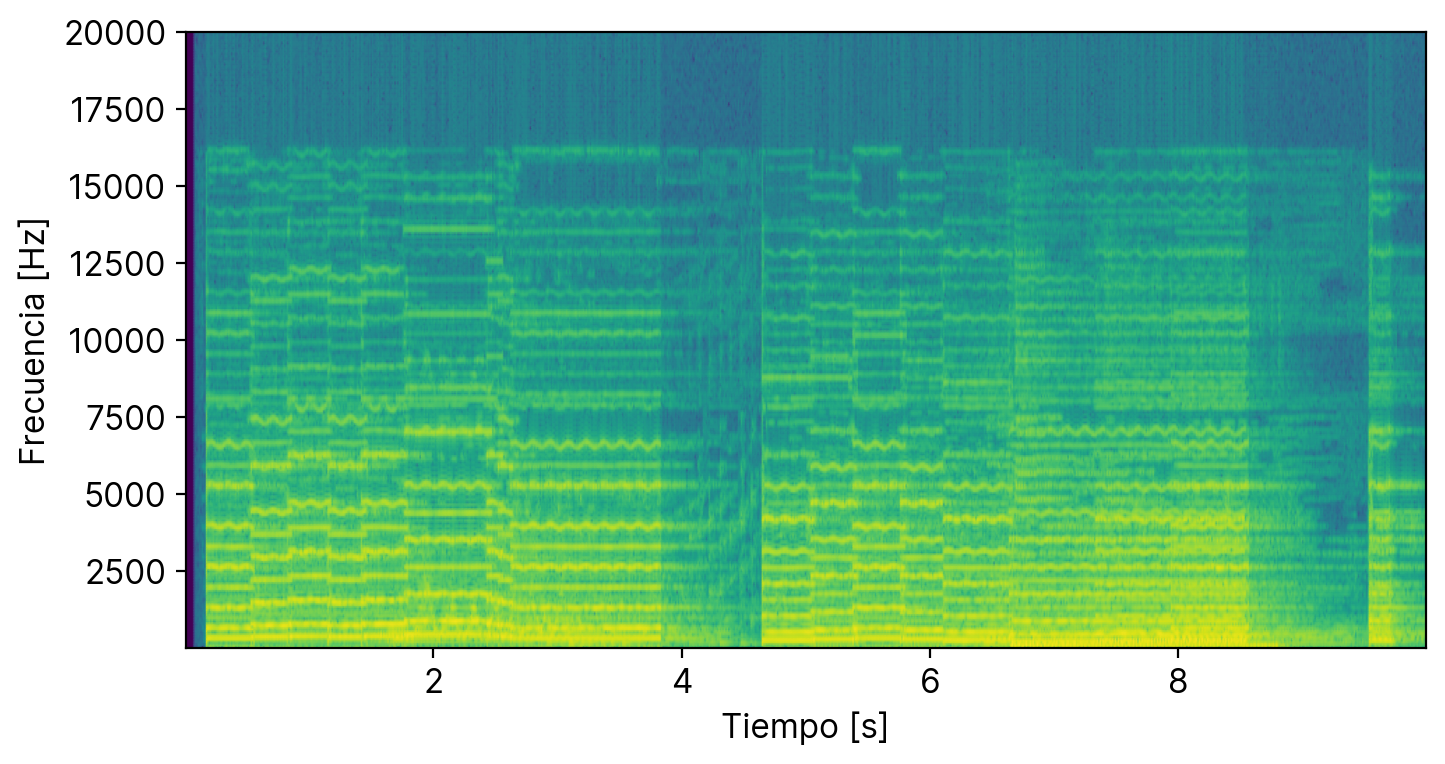
\includegraphics{plot/cancion1_espectograma_bartlett_0512.png}
\caption{Espectrograma primer muestra de ventana triangular de 512 puntos}
\label{cancion1_espectograma_bartlett_0512}
\end{figure}

\begin{figure}[H]
\centering
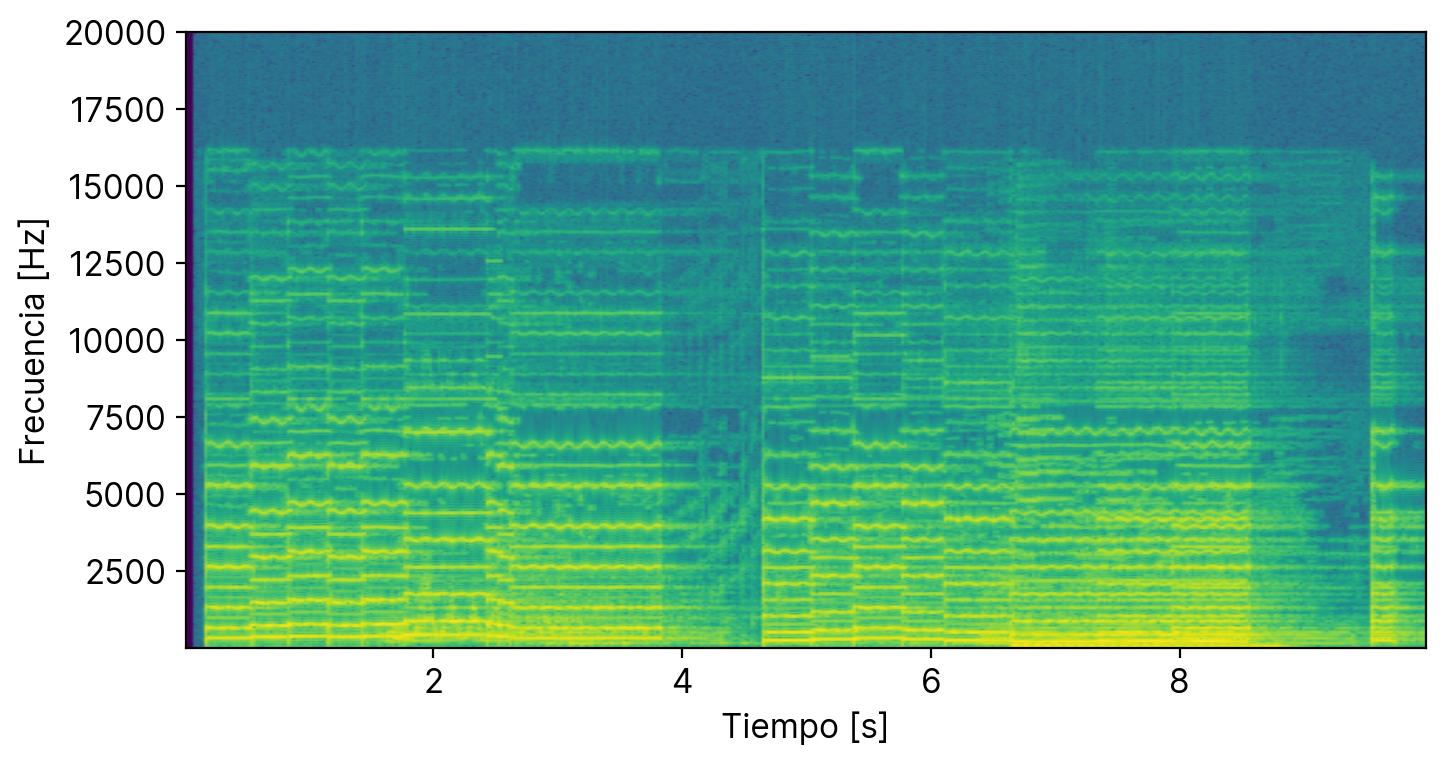
\includegraphics{plot/cancion1_espectograma_bartlett_1024.png}
\caption{Espectrograma primer muestra de ventana triangular de 1024 puntos}
\label{cancion1_espectograma_bartlett_1024}
\end{figure}

\begin{figure}[H]
\centering
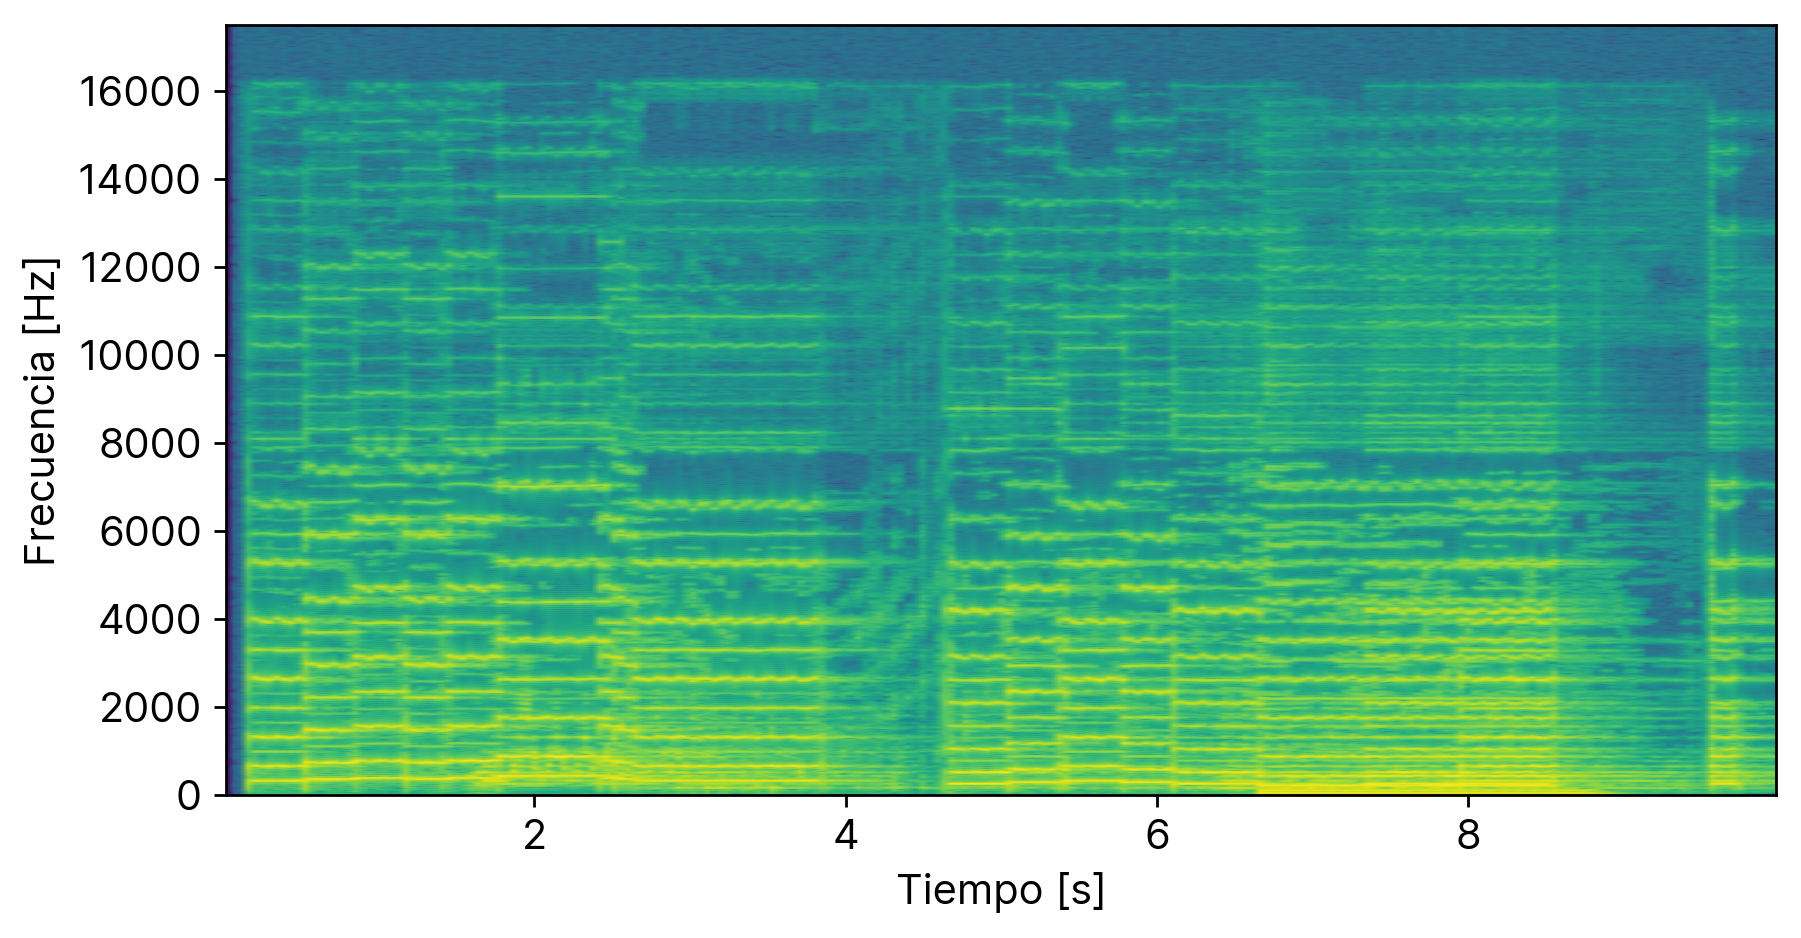
\includegraphics{plot/cancion1_espectograma_bartlett_2048.png}
\caption{Espectrograma primer muestra de ventana triangular de 2048 puntos}
\label{cancion1_espectograma_bartlett_2048}
\end{figure}

\begin{figure}[H]
\centering
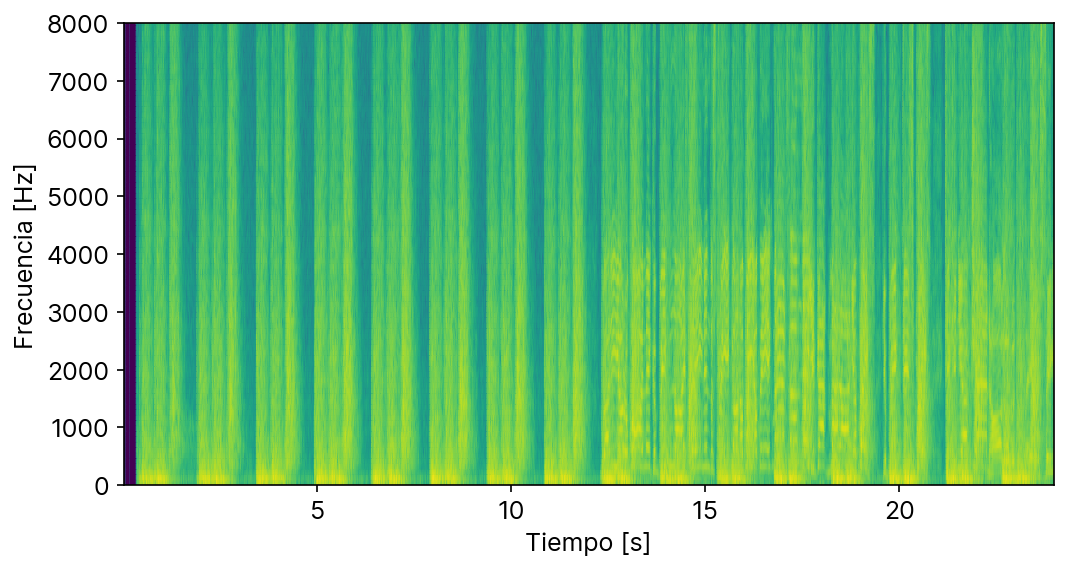
\includegraphics{plot/cancion2_espectograma_bartlett_0512.png}
\caption{Espectrograma segunda muestra de ventana triangular de 512 puntos}
\label{cancion2_espectograma_bartlett_0512}
\end{figure}

\begin{figure}[H]
\centering
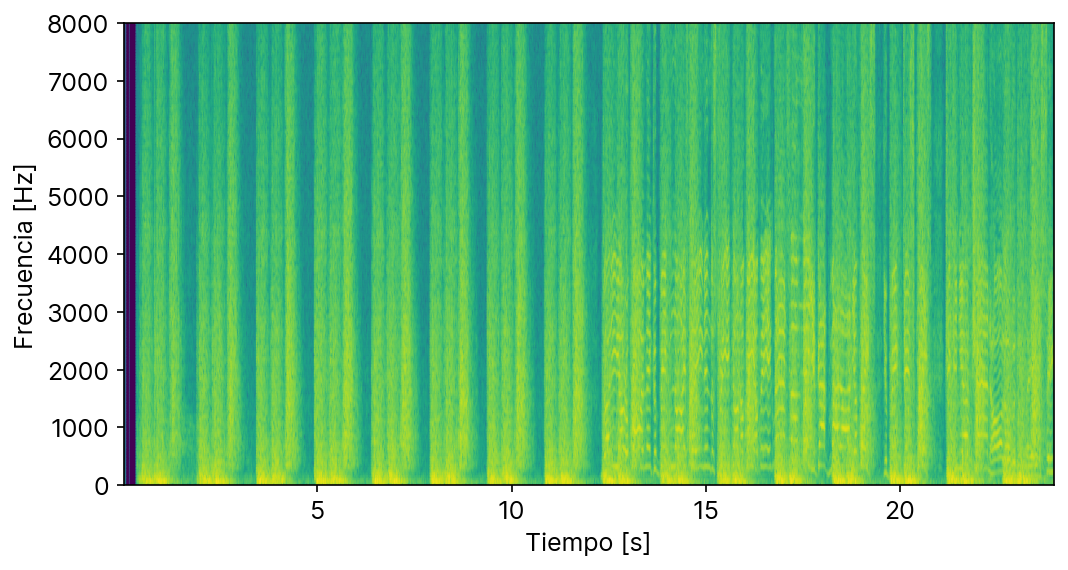
\includegraphics{plot/cancion2_espectograma_bartlett_1024.png}
\caption{Espectrograma segunda muestra de ventana triangular de 1024 puntos}
\label{cancion2_espectograma_bartlett_1024}
\end{figure}

\begin{figure}[H]
\centering
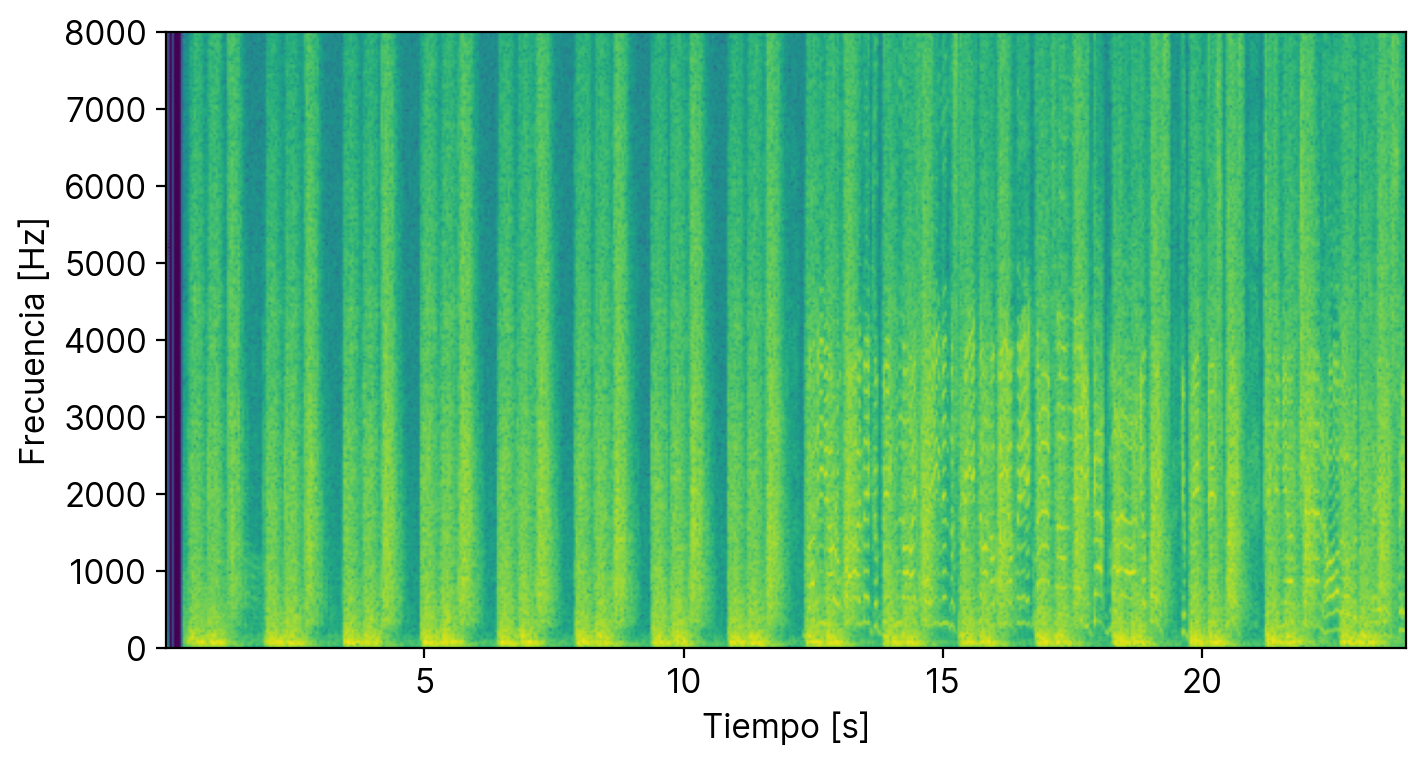
\includegraphics{plot/cancion2_espectograma_bartlett_2048.png}
\caption{Espectrograma segunda muestra de ventana triangular de 2048 puntos}
\label{cancion2_espectograma_bartlett_2048}
\end{figure}

\hypertarget{espectograma-ventana-hann}{%
\subsubsection{Espectrograma con ventana de Hann}\label{espectograma-ventana-hann}}

La ventana de Hann es una funcion que en el dominio temporal tiene una forma
suave, no como la ventana rectangular o triangular que tiene puntos con derivada
discontinua, la forma es parecida a medio ciclo de un seno. En el dominio de
frecuencia, la ventana de Hann tiene una forma parecida a la de la ventana
rectangular con un lobulo principal, pero este mas ancho que el de la
rectangular, esto implica menor resolucion en frecuencia; ademas el espectro de
la ventana de Hann tiene lobulos laterales menores.

\begin{figure}[H]
\centering
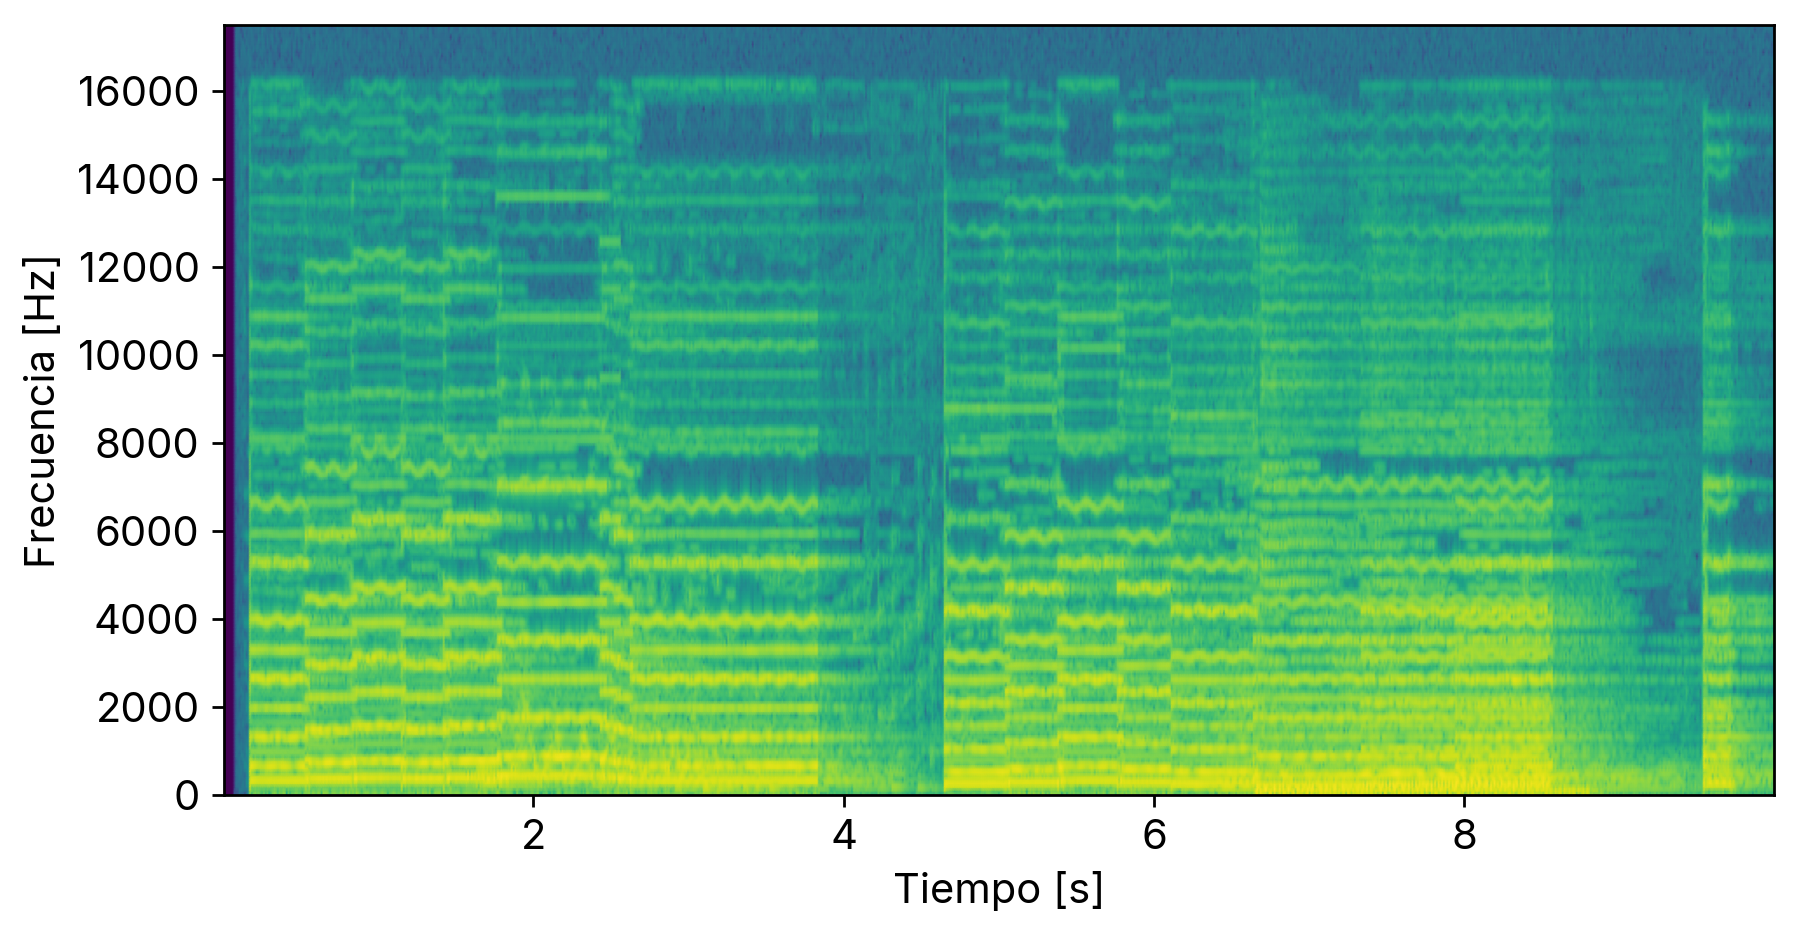
\includegraphics{plot/cancion1_espectograma_hann_0512.png}
\caption{Espectrograma primer muestra con ventana Hann de 512 puntos}
\label{cancion1_espectograma_hann_0512}
\end{figure}

\begin{figure}[H]
\centering
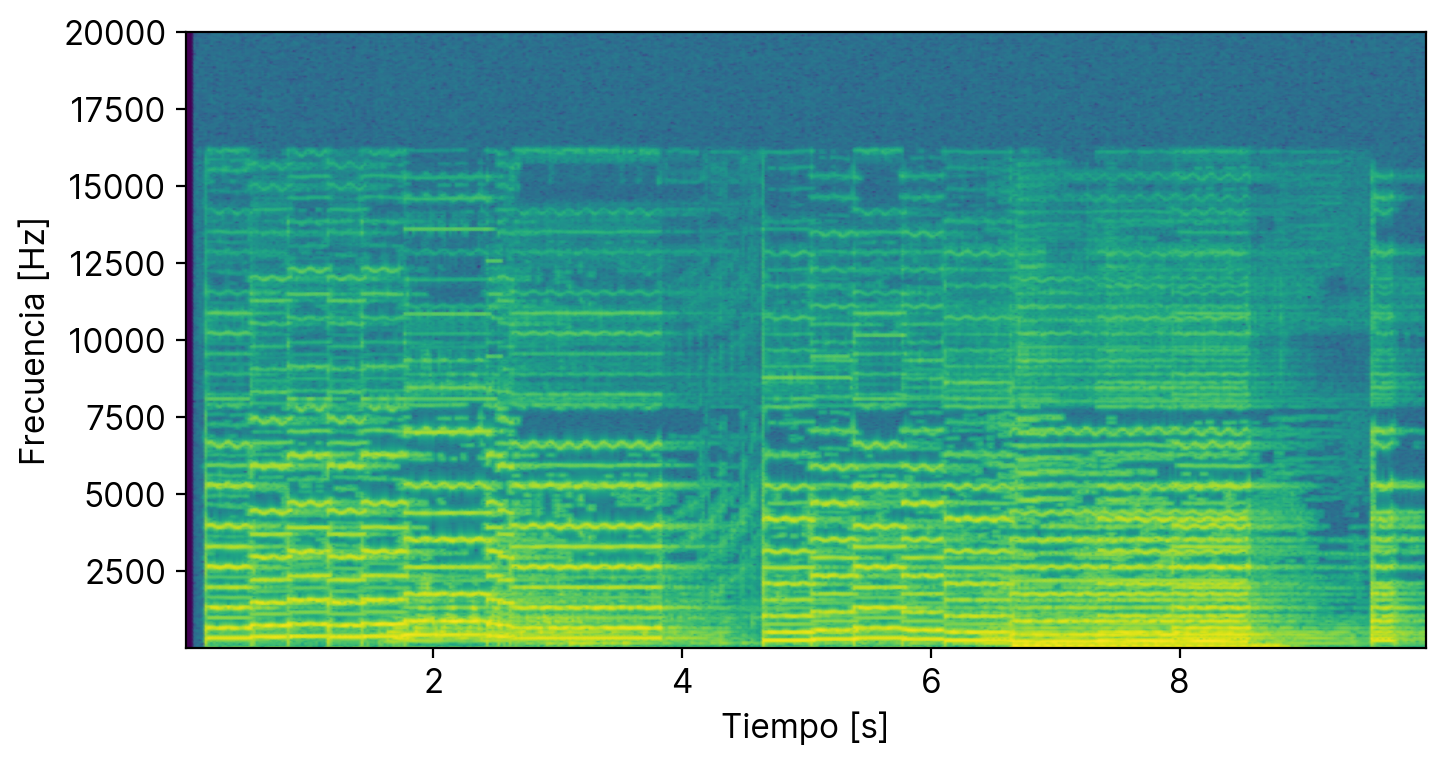
\includegraphics{plot/cancion1_espectograma_hann_1024.png}
\caption{Espectrograma primer muestra con ventana Hann de 1024 puntos}
\label{cancion1_espectograma_hann_1024}
\end{figure}

\begin{figure}[H]
\centering
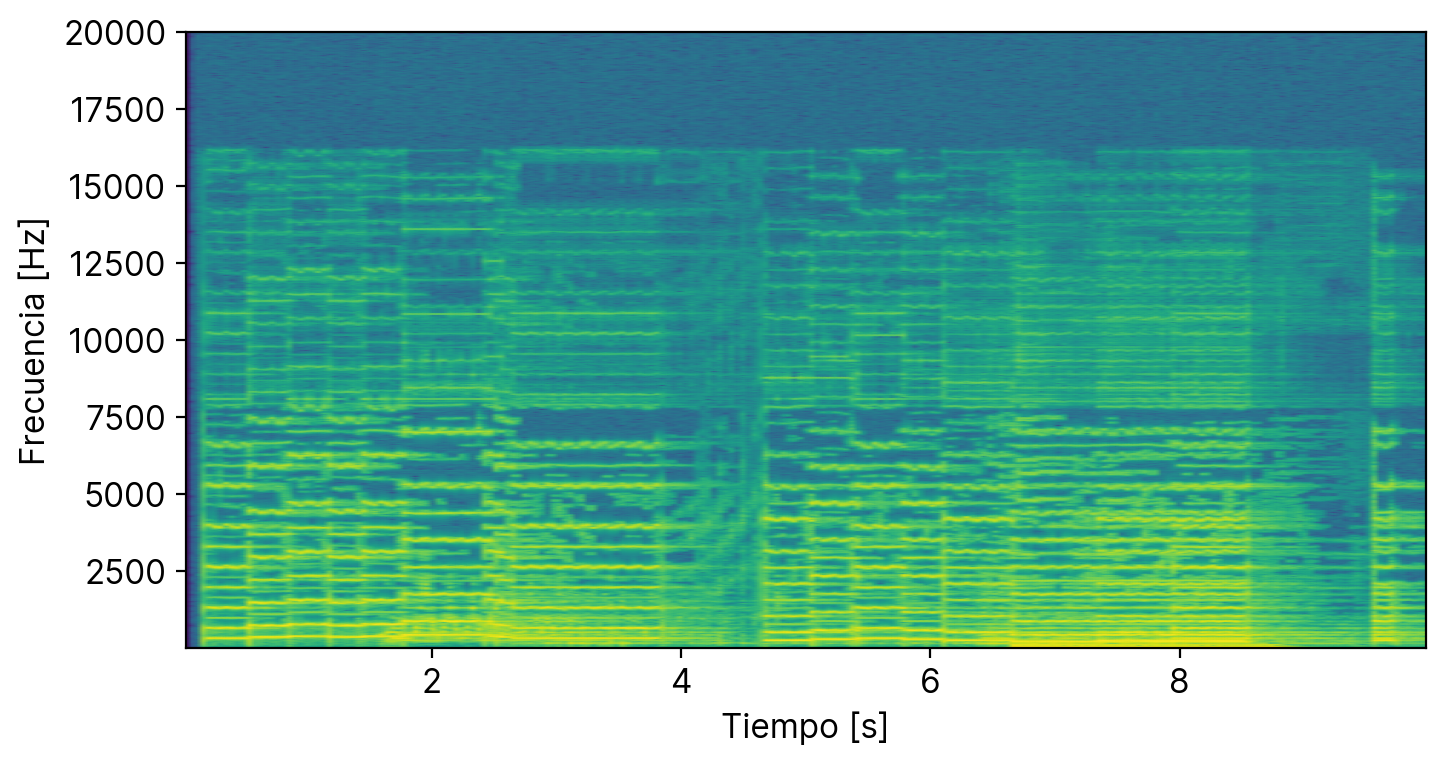
\includegraphics{plot/cancion1_espectograma_hann_2048.png}
\caption{Espectrograma primer muestra con ventana Hann de 2048 puntos}
\label{cancion1_espectograma_hann_2048}
\end{figure}

\begin{figure}[H]
\centering
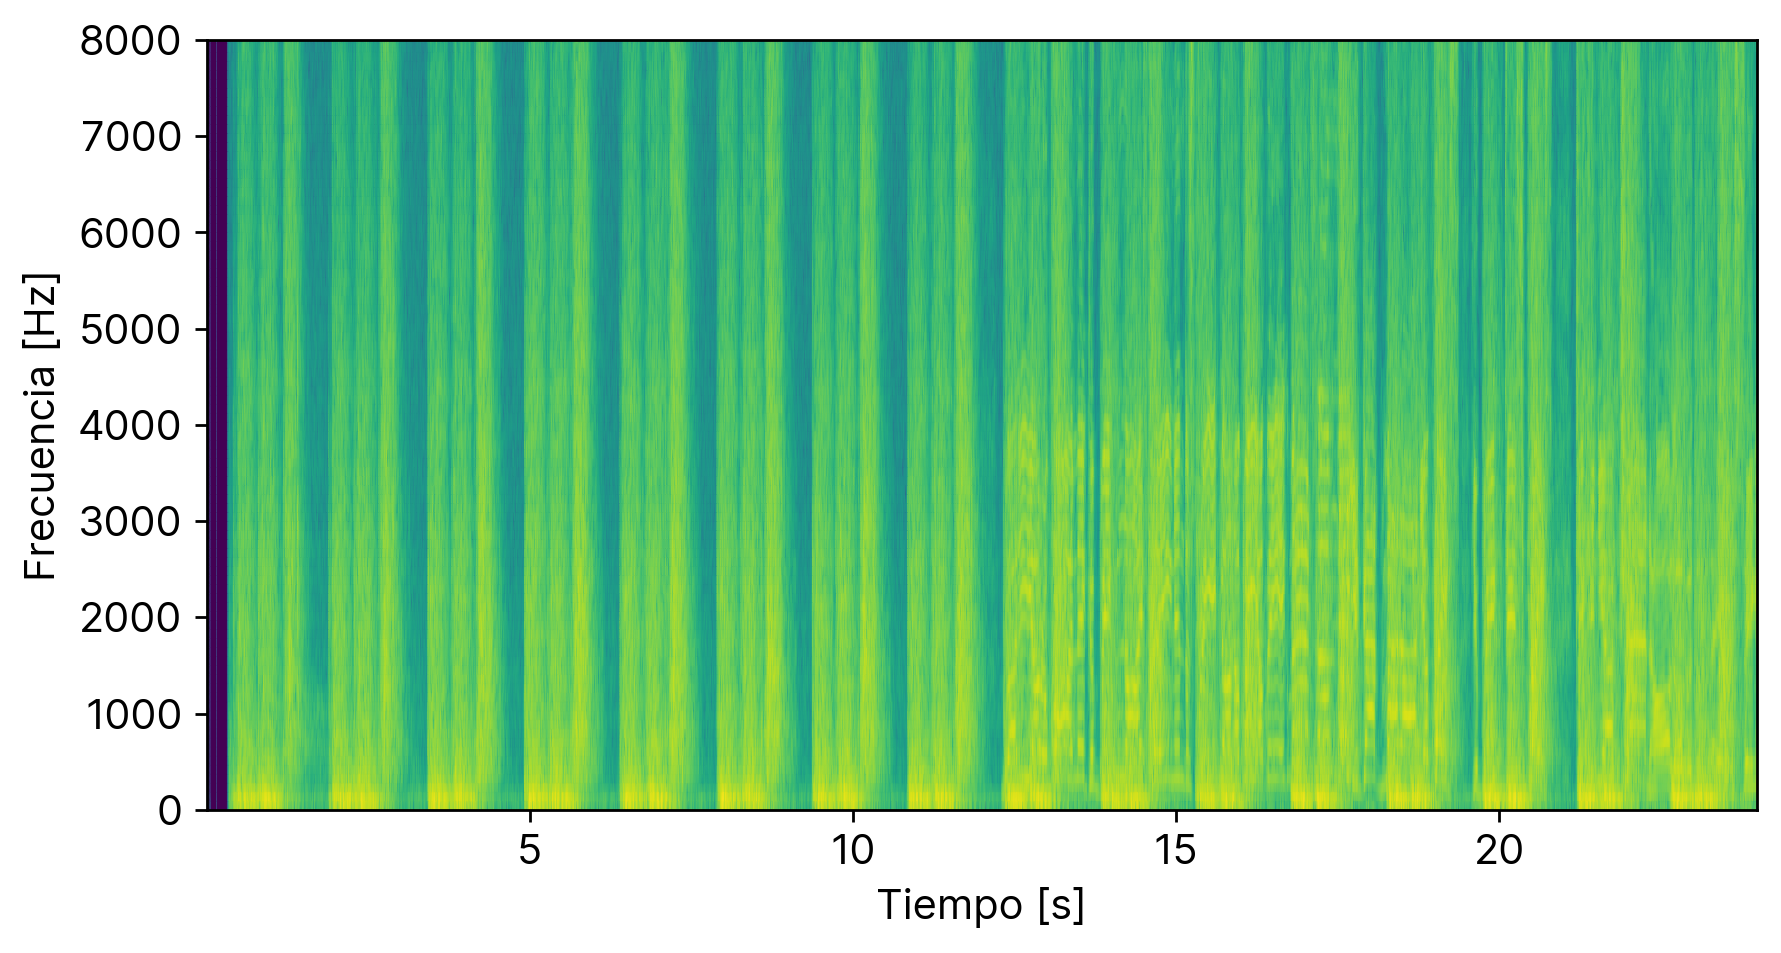
\includegraphics{plot/cancion2_espectograma_hann_0512.png}
\caption{Espectrograma segunda muestra con ventana Hann de 512 puntos}
\label{cancion2_espectograma_hann_0512}
\end{figure}

\begin{figure}[H]
\centering
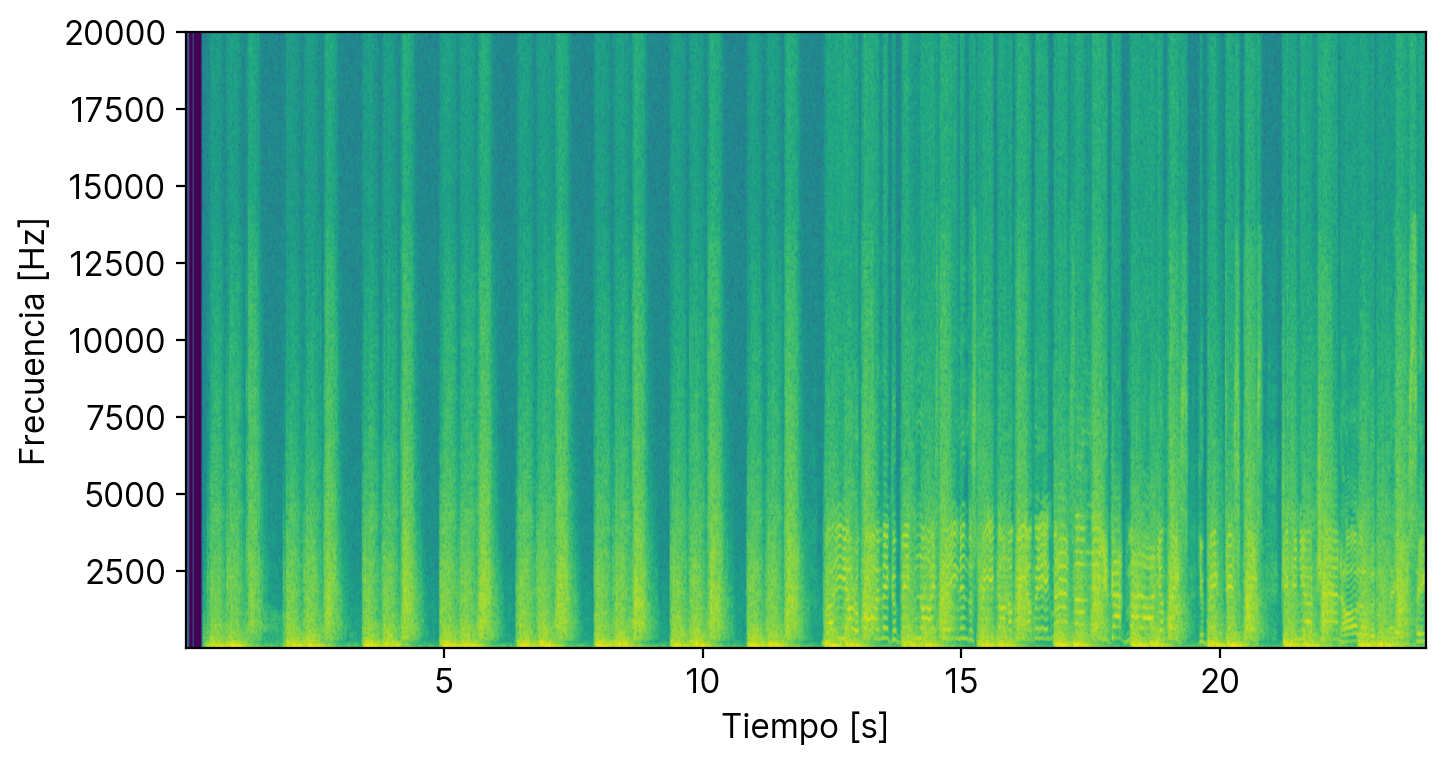
\includegraphics{plot/cancion2_espectograma_hann_1024.png}
\caption{Espectrograma segunda muestra con ventana Hann de 1024 puntos}
\label{cancion2_espectograma_hann_1024}
\end{figure}

\begin{figure}[H]
\centering
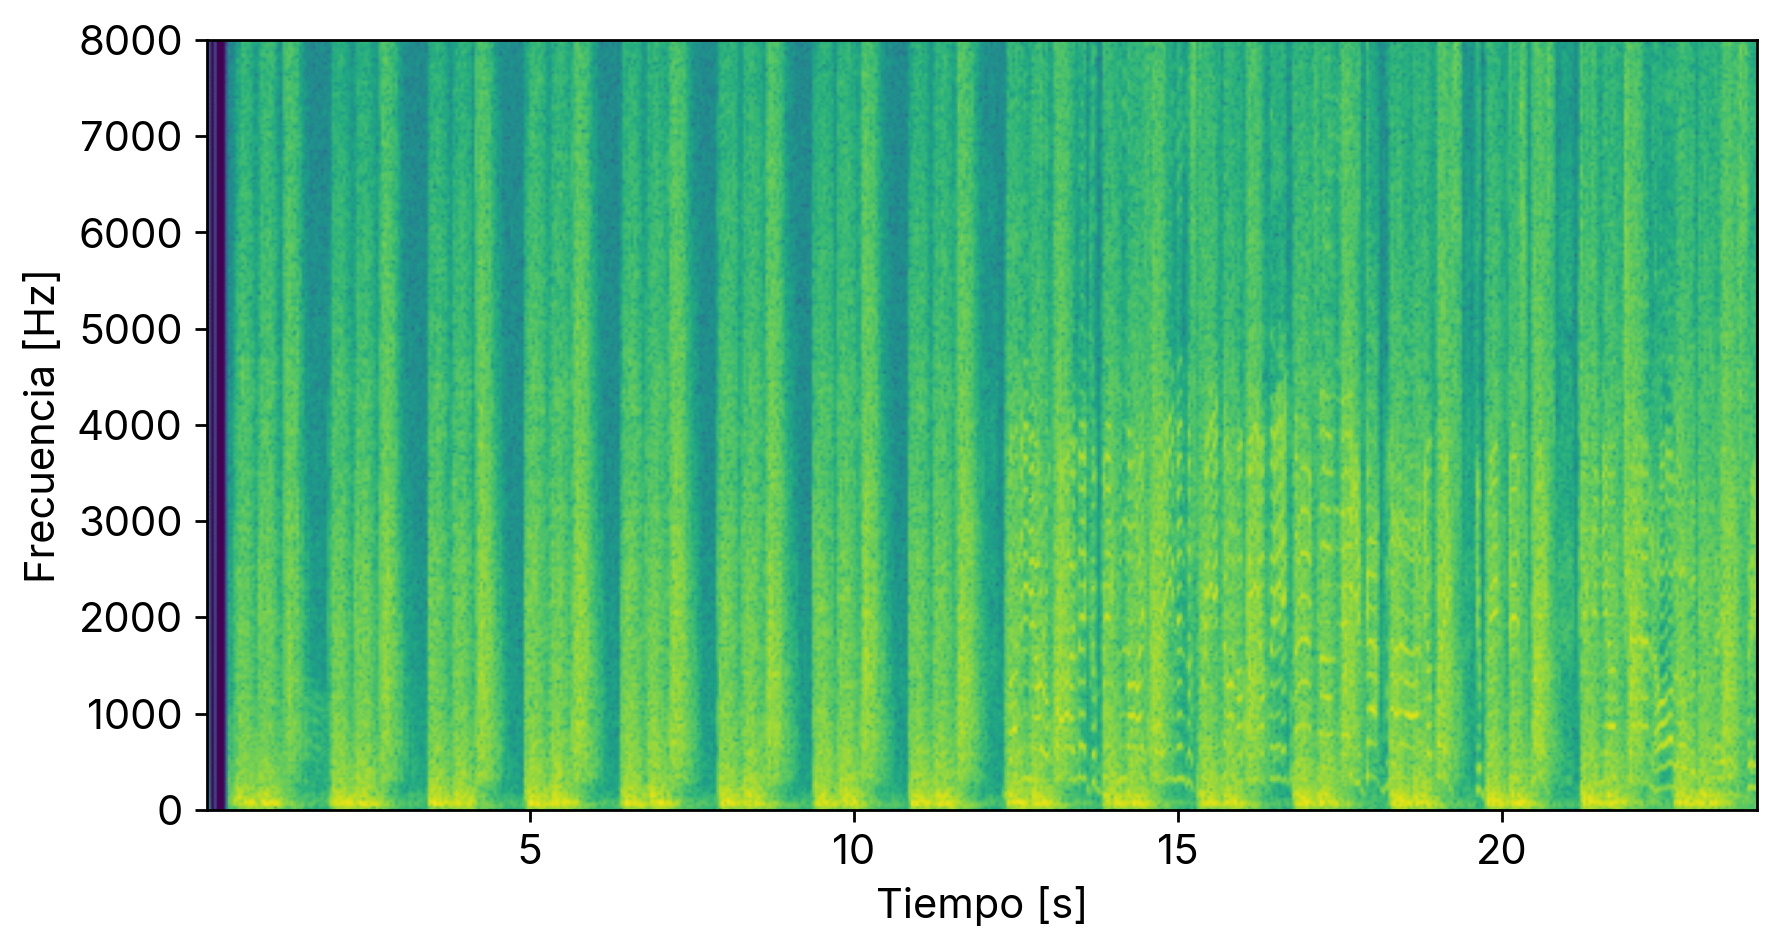
\includegraphics{plot/cancion2_espectograma_hann_2048.png}
\caption{Espectrograma segunda muestra con ventana Hann de 2048 puntos}
\label{cancion2_espectograma_hann_2048}
\end{figure}

Analizando el espectrograma de la primer canción, en particular el de la figura \ref{cancion1_espectograma_bartlett_2048}, en el cual se toman 2048 puntos y se utiliza una ventana triangular, se observa claramente las notas que componen la melodía, y ademas en que tiempo ocurre cada una de ellas. Ademas se observa que no es muy clara la resolución temporal pero de todas maneras se tiene una aproximación general de en que tiempo ocurre cada nota, para mayor resolución se puede observar u analizar la figura \ref{cancion1_espectograma_bartlett_0512} en la cual se toman menos puntos, por lo tanto se tiene mayor resolución temporal.

\hypertarget{Efectos-musicales-en-términos-de-sistemas}{%
\subsection{Efectos musicales en términos de sistemas}\label{Efectos-musicales-en-términos-de-sistemas}}

En esta sección se analizan distintos efectos interpretándolos como sistemas que procesan la señal de entrada x(t) dando en la salida una señal y(t). 
Se trabaja con una señal senoidal pura de 440Hz, implementando los efectos de manera digital mediante código. En cada caso se grafican los espectros resultantes de aplicar los distintos efectos a la señal original.

\subsubsection{Delay}

El efecto del \textit{delay} consiste en sumar a la señal original una copia de sí misma con un factor de retroalimentación que genera repeticiones. Puede modelarse como:

\[
y[n] = x[n] + \alpha\, y[n - D]
\]

donde $D$ representa el retardo en muestras y $\alpha$ es el coeficiente de retroalimentación.

Analizando las propiedades de este sistema, se observa que es un sistema \textbf{lineal}, posee \textbf{memoria} ya que depende de muestras pasadas, y es \textbf{invariante en el tiempo} debido a que el retardo no cambia a lo largo del tiempo.

\begin{figure}[H]
    \centering
    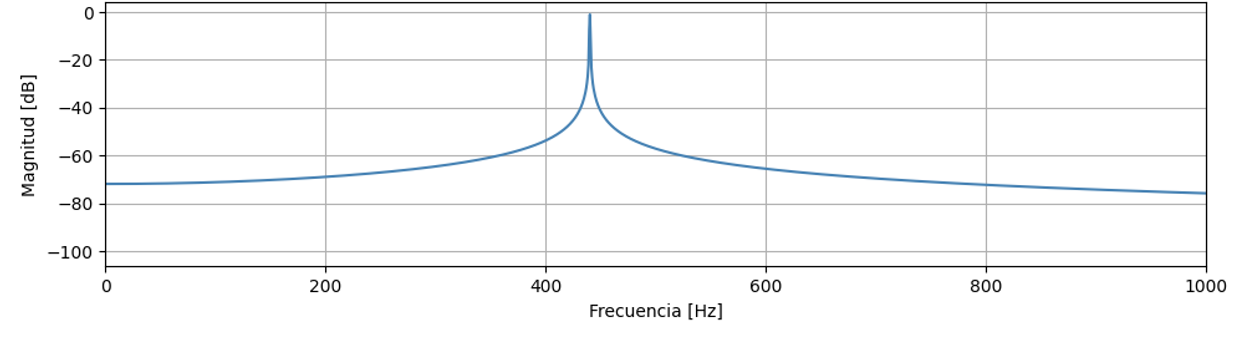
\includegraphics[width=0.75\linewidth]{plot/delay_original.png}
    \caption{Espectro original}
    \label{delay_original}
\end{figure}

\begin{figure}[H]
    \centering
    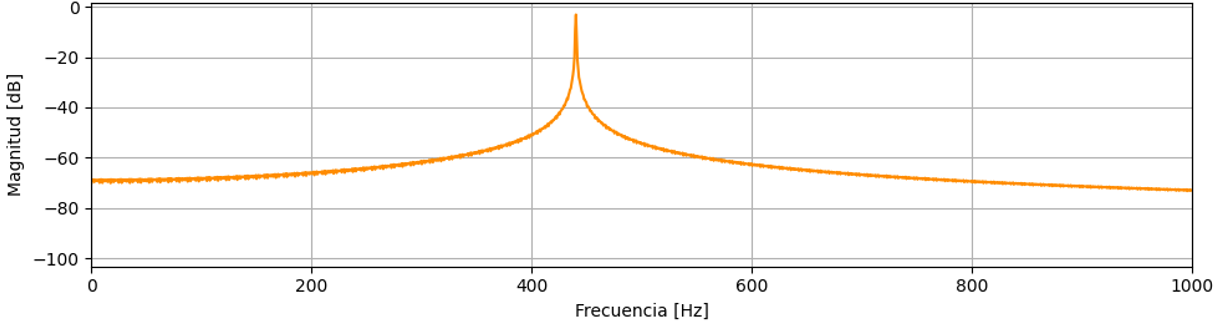
\includegraphics[width=0.75\linewidth]{plot/delay_efecto.png}
    \caption{Espectro con efecto delay}
    \label{delay_efecto}
\end{figure}

\subsubsection{Distorsión}

La distorsión consiste en aplicar una función no lineal sobre la amplitud de la señal, como puede ser un recorte (clipping). En este caso se utiliza la función tangente hiperbólica:

\[
y[n] = tanh(Gx[n])
\]

Este sistema no es lineal ya que su salida no es proporcional a la entrada, es invariante en el tiempo ya que no cambia en el tiempo, y es sin memoria porque cada muestra depende solo de la muestra actual.
Se observa la aparición de armónicos múltiples de la frecuencia fundamental, dando un tono mas brillante y enriquecido.

\begin{figure}[H]
    \centering
    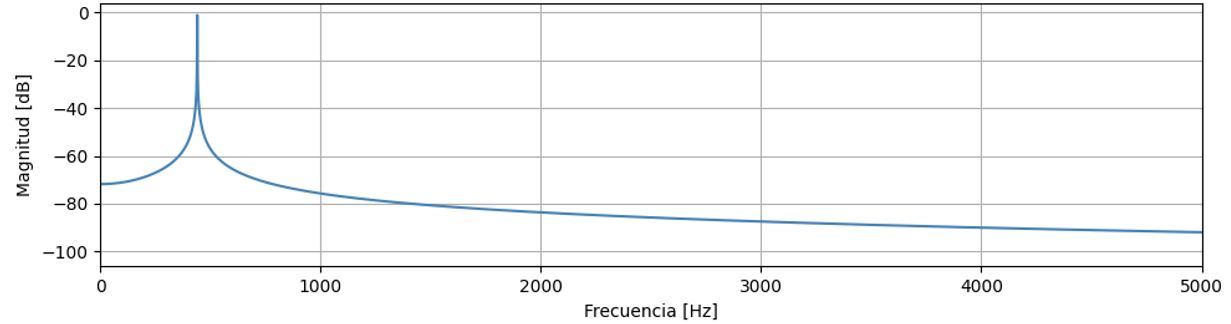
\includegraphics[width=0.75\linewidth]{plot/distorsion_original.png}
    \caption{Espectro original}
    \label{distorsion_original}
\end{figure}

\begin{figure}[H]
    \centering
    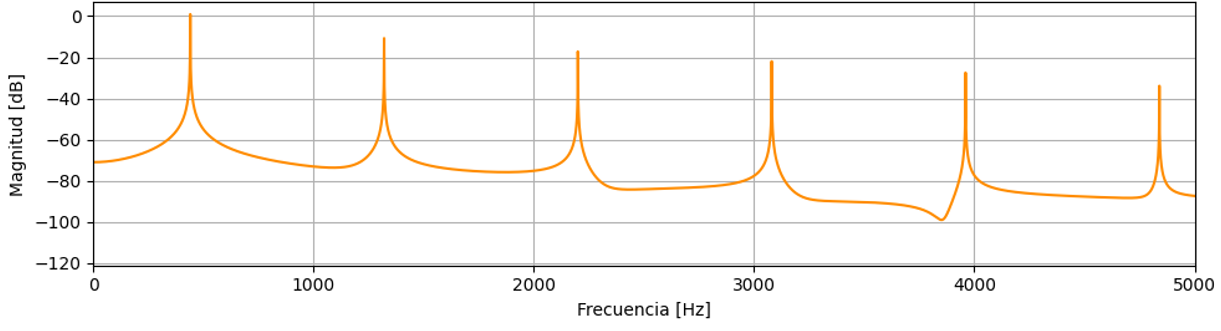
\includegraphics[width=0.75\linewidth]{plot/distorsion_efecto.png}
    \caption{Espectro con efecto distorsión}
    \label{distorsion_efecto}
\end{figure}

\subsubsection{Trémolo}

Consiste en la modulación de la amplitud de la señal, es decir, en variar su volumen en forma periódica mediante un oscilador. Se implementa mediante

\[
y[n] = \left( 1 - d \, \sin\left( \frac{2\pi f_m n}{f_s} \right) \right) x[n]
\]

donde $d$ es la profundidad de modulación y $f_m$ la frecuencia de modulación.

El sistema implementado es \textbf{lineal}, \textbf{invariante en el tiempo} (si la frecuencia de modulación es constante) y \textbf{tiene memoria}, ya que depende de una función periódica externa.  

En el espectro de la señal se pueden observar \textit{bandas laterales} que rodean la frecuencia fundamental, producidas por la modulación en amplitud.

\begin{figure}[H]
    \centering
    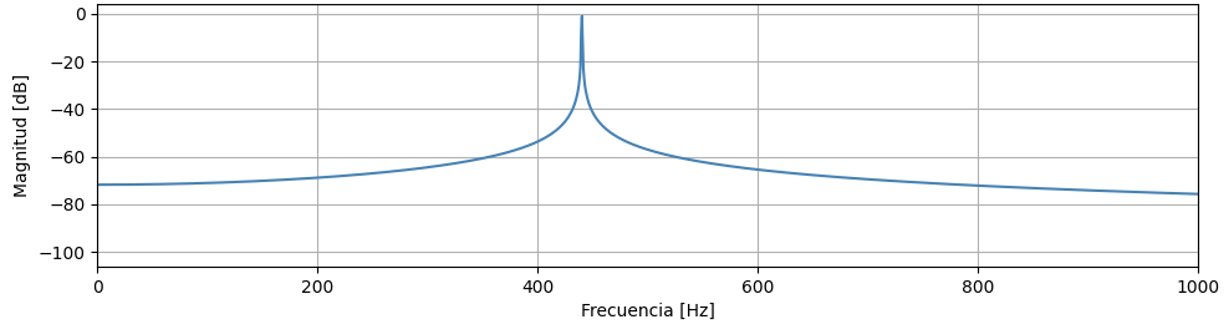
\includegraphics[width=0.75\linewidth]{plot/trembolo_original.png}
    \caption{Espectro nota original}
    \label{trembolo_original}
\end{figure}

\begin{figure}[H]
    \centering
    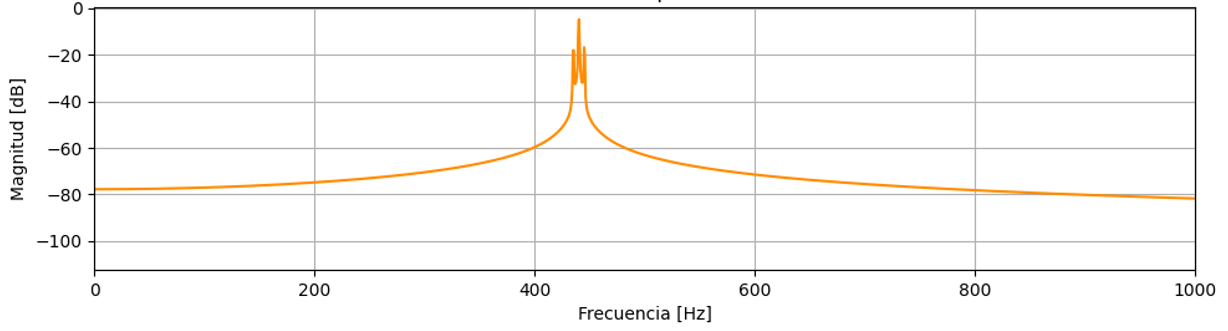
\includegraphics[width=0.75\linewidth]{plot/trembolo_efecto.png}
    \caption{Espectro nota con efecto tremolo}
    \label{trembolo_efecto}
\end{figure}

\subsubsection{Vibrato}

Produce una modulación en frecuencia, alterando la frecuencia instantánea de la señal. Se lo puede expresar como un retardo variable en el tiempo:

\[
y[n] = x\!\left[n + d \, \sin\!\left( \frac{2\pi f_m n}{f_s} \right)\right]
\]

Se observa que este sistema \textbf{no es lineal}, ya que el desplazamiento depende de la señal moduladora.  
Es \textbf{invariante en el tiempo} (si el modulador es constante) y \textbf{tiene memoria}, ya que utiliza muestras pasadas.  

En el espectro se puede apreciar un \textit{ensanchamiento} en la frecuencia fundamental con variaciones periódicas alrededor de la misma, lo que refleja la modulación del tono.

\begin{figure}[H]
    \centering
    \includegraphics[width=0.75\linewidth]{plot/vibrato_original.png}
    \caption{Espectro original}
    \label{vibrato_original}
\end{figure}

\begin{figure}[H]
    \centering
    \includegraphics[width=0.75\linewidth]{plot/vibrato_efecto.png}
    \caption{Espectro con efecto vibrato}
    \label{vibrato_efecto}
\end{figure}

\subsection*{Chorus}

Combina múltiples copias de la señal, cada una con un retardo distinto.  
Simula varios instrumentos sonando al mismo tiempo.  
Se lo puede modelar como la suma de varios vibratos:

\[
y[n] = \frac{1}{N} \sum_{k=1}^{N} x\!\left[n + d_k \sin\!\left( \frac{2\pi f_{m_k} n}{f_s} \right)\right]
\]

Es un sistema \textbf{no lineal} debido a la interpolación variable,  
\textbf{invariante en el tiempo} (si los parámetros son constantes) y \textbf{tiene memoria} debido al retardo de cada instrumento.  

En el espectro se observa un \textit{ensanchamiento} alrededor de la frecuencia fundamental  
y una estructura densa debido a la suma de fuentes sonoras.


\begin{figure}[H]
    \centering
    \includegraphics[width=0.75\linewidth]{plot/chorus_original.png}
    \caption{Espectro original}
    \label{chorus_original}
\end{figure}

\begin{figure}[H]
    \centering
    \includegraphics[width=0.75\linewidth]{plot/chorus_efecto.png}
    \caption{Espectro con efecto chorus}
    \label{chorus_efecto}
\end{figure}

Cada efecto puede interpretarse como un sistema que transforma una señal de entrada aplicando operaciones de retardo, modulación o no linealidad. Los efectos que se caracterizaron como lineales e invariantes en el tiempo (delay y trembolo) modifican el espectro de manera predecible. Mientras que los no lineales introducen componentes que afectan la estructura armónica que se tenía en la señal original


\iffalse
% commentado

\hypertarget{Gráfico-temporal-y-espectrograma-de-una-melodía-musical}{%
\subsubsection{Gráfico temporal y espectrograma de una melodía musical}\label{Gráfico-temporal-y-espectrograma-de-una-melodía-musical}}

\fi


\end{document}